\ifx\XeTeXversion\undefined
\pdfoutput=1
\fi
\documentclass[conference]{IEEEtran}
\IEEEoverridecommandlockouts

\ifx\XeTeXversion\undefined
\usepackage[T1]{fontenc}
\usepackage{tgtermes}
\usepackage{tgheros}
\usepackage[scale=0.84]{tgcursor}
\else
\usepackage{fontspec}
\setmainfont{texgyretermes-regular.otf}[
  BoldFont=texgyretermes-bold.otf,
  ItalicFont=texgyretermes-italic.otf,
  BoldItalicFont=texgyretermes-bolditalic.otf,
  SmallCapsFeatures={Letters=SmallCaps}
]
\setsansfont{texgyreheros-regular.otf}[
  BoldFont=texgyreheros-bold.otf,
  ItalicFont=texgyreheros-italic.otf,
  BoldItalicFont=texgyreheros-bolditalic.otf
]
\setmonofont{texgyrecursor-regular.otf}[
  BoldFont=texgyrecursor-bold.otf,
  ItalicFont=texgyrecursor-italic.otf,
  BoldItalicFont=texgyrecursor-bolditalic.otf,
  SmallCapsFont=texgyrecursor-regular.otf,
  Scale=0.84
]
\fi

\usepackage{cite}
\usepackage{enumitem}
\usepackage{amsmath,amssymb,amsfonts}
\usepackage{graphicx}
\usepackage{textcomp}
\usepackage{xcolor}
\usepackage{tikz}
\usetikzlibrary{shapes.geometric,arrows.meta,positioning,fit,backgrounds,calc}
\usepackage{booktabs}
\usepackage{multirow}
\usepackage{array}
\usepackage{placeins}
\usepackage{url}
\usepackage[hidelinks]{hyperref}

\AddToHook{env/thebibliography/begin}{\label{ReferencesStart}}

\definecolor{accentblue}{RGB}{70,130,180}
\definecolor{accentred}{RGB}{220,20,60}
\definecolor{accentgreen}{RGB}{50,150,50}
\definecolor{accentpurple}{RGB}{128,0,128}
\definecolor{accentorange}{RGB}{255,140,0}

\begin{document}

\title{The Jung--Plato Lattice: Multi-Family Representation Denoising, Compositional Probing, and Cross-Tokenizer Distillation}

\author{
  \IEEEauthorblockN{Benjamin Babeshkin}
  \IEEEauthorblockA{
    Independent Research (\texttt{syn-ack-ai})\\
    Preprint DOI: \url{https://doi.org/10.5281/zenodo.24572076}\\
    Code \& Data: \url{https://github.com/syn-ack-ai/jung-plato-lattice}
  }
}

\maketitle

\begin{abstract}
Independently trained language models use different tokenizers, datasets, and architectures, yet their middle-layer activations align across families. Recording clause-ending states across five open-weight families (Gemma 4 E4B, Qwen3.5 9B, Llama 3.1 8B, Mistral 7B, and looped Inkling 2 Mini) and aligning them via 10-iteration Generalized Procrustes Analysis yields a 256-dimensional consensus (\texttt{C5}). On two excluded target families (Phi-4-mini, OLMo 3 7B), \texttt{C5} predicts held-out activations by $+8.3$ and $+7.8$ strict $R^2_{\text{opt}}$ points ($+11.3$ and $+10.4$ Frobenius $R^2_{\text{frob}}$ points) above every teacher. Supervising one middle layer via a discarded linear head transfers this geometry across tokenizers with zero added inference parameters at 5M scale ($+15$ to $+23$ $R^2_{\text{frob}}$ points, mixed downstream scores) and on 8B multimodal Gemma 4 E4B. On 240 actor-intent swaps where seven fitted linear lexical and polarity baselines sit at 50.0\% (though an actor-lexicon times polarity rule hits 95.5\%--96.3\%), mean-pooled cross-family readout rises from 30\% to its observed peak at 50\% depth (73.0\% Gemma / 73.1\% Qwen overall, 64.4\% / 58.3\% adverse, 26.0\% / 28.2\% all-four-right vs.\ 6.25\% chance), while single-layer steering gives a null effect. Transplanting rival-only 50\%-depth \texttt{C3\_50} (zero Gemma 4) into Gemma 4 E4B layers 19--20 across three paired seeds lifts held-out-family alignment over matched control ($+0.0869$ Phi-4, $+0.0780$ OLMo 3 $R^2_{\text{frob}}$) without improving probing or MCQ. On 480 cleaned historical folktales, predicted archetype-to-division pairings fail ($\cos=-0.106, p=0.952$) and unlabeled PCA matches or beats study-selected Jungian labels, though labels slightly exceed shuffles ($p_{\text{holm}}=0.0417$). Making no claim about machine consciousness or psyche, we study aligned subspaces as statistical projections of human cultural data.
\end{abstract}

\begin{IEEEkeywords}
Plato, Platonic eidos, Platonic Representation Hypothesis, Carl Jung, Jungian archetypes, analytical psychology, comparative mythology, narrative geometry, Generalized Procrustes Analysis, Orthogonal Procrustes, cross-tokenizer distillation, mechanistic interpretability, epistemic uncertainty.
\end{IEEEkeywords}

\section{Introduction}
Five open-weight large language models (LLMs) trained by five different organizations read the same public passages while we record their middle-layer activations at matching clause endings. Rotating their coordinate systems into a common frame and averaging them produces one 256-dimensional consensus space (\texttt{C5}). After fitting a sixth or seventh model's principal component basis on the training corpus and calibrating one linear rotation on half of its held-out passages, \texttt{C5} predicts the remaining activations of that excluded model better than any single 7B--9B teacher.

This result sits at the intersection of representation alignment in machine learning, classical philosophy, and analytical psychology. Independent laboratories train LLMs with separate tokenizers, data mixtures, and architectures, yet their hidden spaces converge under the \textit{Platonic Representation Hypothesis} (PRH) \cite{huh2024platonic,balestriero2026proving}. Plato contrasted shifting shadows with invariant Forms (\textit{eidos}):
\begin{quote}
\small
``To them, I said, the truth would be literally nothing but the shadows of the images'' (\textit{Republic} VII, 515c). Asking about the underlying Forms, Socrates asks: ``are these essences, I say, liable at times to some degree of change? or are they each of them always what they are, having the same simple self-existent and unchanging forms, not admitting of variation at all, or in any way, or at any time?'' \cite{plato1892dialogues} (\textit{Phaedo}, 78d)
\end{quote}
In \textit{Plato's Key}, Cheng et al.~\cite{cheng2026platoskey} moved from passive similarity to direct intervention. Using closed-form Orthogonal Procrustes rotation \cite{schonemann1966procrustes} with one global Frobenius scale factor, they swapped factual-recall vectors between frozen LLMs at 22--38\% depth and found that the top 256 principal components (PCs) retained a median 74\% of the full-rotation transfer accuracy.

Nearly a century earlier, Carl Jung called recurring structural patterns (\textit{archetypes}) ``an explanatory paraphrase of the Platonic \textit{eidos}'' (transliterated from Greek) \cite{jung1968archetypes} (CW 9.I, \P5). He distinguished formal predisposition from inherited pictures:
\begin{quote}
\small
``Its form, however, as I have explained elsewhere, might perhaps be compared to the axial system of a crystal, which, as it were, preforms the crystalline structure in the mother liquid, although it has no material existence of its own. This first appears according to the specific way in which the ions and molecules aggregate. The archetype in itself is empty and purely formal, nothing but a \textit{facultas praeformandi}, a possibility of representation which is given a priori.'' \cite{jung1968archetypes} (CW 9.I, \P155)
\end{quote}
Jung separated the \textit{archetype-as-such}, an irrepresentable formal constraint \cite{jung1969structure} (CW 8, \P417) placed ``beyond the psychic sphere, analogous to the position of physiological instinct, which is immediately rooted in the stuff of the organism'' \cite{jung1969structure} (CW 8, \P420), from concrete \textit{archetypal images}. Jung argued that ``the representations themselves are not inherited, only the forms'' \cite{jung1968archetypes} (CW 9.I, \P155), whereas later scholars emphasized cultural transmission \cite{roesler2012archetypes} or developmental emergence \cite{hogenson2001baldwin,knox2003archetype}, alongside associative complexes studied in Jung's 1904--1909 Word Association Test (WAT) \cite{jung1973experimental,jung1976symbolic}. Our measurements test neither subjective experience, consciousness, nor biological inheritance \cite{butlin2023consciousness,shanahan2024talking}. We make no claim either way about machine consciousness or psyche, and analyze aligned subspaces strictly as statistical projections of human-authored training data (text, plus images or audio for multimodal models such as Gemma 4 \cite{gemmateam2026gemma4}, Qwen3.5 \cite{qwen2026qwen35}, and Inkling 2 Mini \cite{thinkingmachines2026inkling}).

Because this study addresses both machine learning engineers and psychologists, we briefly translate core terms across both fields before stating our research questions. For psychology readers: an LLM's \textit{hidden state} is a list of numbers representing how a model internally encodes a passage at a given processing depth; \textit{principal component analysis} (PCA) compresses those thousands of numbers into the 256 directions that vary most across passages; a \textit{Procrustes rotation} rigidly rotates one model's coordinate axes to line up with another's without stretching individual dimensions; \textit{bag-of-words} (BoW) counts individual words while ignoring grammar and word order; and \textit{valence projection} subtracts general good-versus-bad emotional tone from the internal vectors so we can see what remains. For machine learning engineers: Jung's \textit{archetype-as-such} is an unobservable structural constraint, distinct from any specific character or plot; the \textit{Aarne--Thompson--Uther} (ATU) index \cite{uther2004types} is the standard folklorist catalog grouping international folktales by plot type; and the \textit{Word Association Test} measures whether emotionally charged cues disturb response timing or subsequent neutral trials.

Prior work established Orthogonal Procrustes \cite{schonemann1966procrustes}, Generalized Procrustes Analysis (GPA) \cite{gower1975gpa}, cortical hyperalignment \cite{haxby2011hyperalignment}, relative latent communication \cite{moschella2023relative}, multi-way and five-architecture GPA \cite{achara2026multiway,anthonio2026five}, cross-tokenizer distillation and model fusion \cite{boizard2025uld,wan2024fusellm}, event-knowledge probing \cite{kauf2023event}, neighbor-graph convergence \cite{huh2024platonic}, joint-embedding identifiability \cite{balestriero2026proving}, and pairwise key transfer \cite{cheng2026platoskey}. Building on those foundations, we investigate five empirical questions:
\begin{enumerate}
  \item \textbf{Multi-family consensus denoising:} Does 10-iteration GPA across five unrelated families predict two excluded target families (seven organizations total) better than any single teacher?
  \item \textbf{Depth locus and actor-intent readout (Claims A and B):} How does cross-family linear readout change across depth when seven fitted, setting-disjoint linear lexical and polarity baselines sit at 50.0\%, and how does it compare with explicit actor-by-polarity rules and causal steering?
  \item \textbf{Zero-overhead cross-tokenizer and rival-only 50\%-depth distillation:} Can supervising one middle layer through a discarded linear head transfer 256-dimensional consensus geometry at 5M scale and on 8B multimodal Gemma 4 E4B, including a rival-only 50\%-depth transplant (\texttt{C3\_50}) that removes Gemma 4 from its own teacher?
  \item \textbf{Historical folklore and role-taxonomy boundaries (Claim C):} On independently indexed ATU folktales \cite{uther2004types,hagedorn2022bearing}, do study-selected Jung-inspired narrative roles beat predicted pairings, unlabeled PCA, family roles, or ordinary workplace roles?
  \item \textbf{Epistemic probing and negative audits:} When conversational prompting alters first-token entropy, how much internal known-versus-unknown separation comes from evaluative sentiment versus coherence, and which follow-up probes fail strict audits?
\end{enumerate}

Section~\ref{sec:related} reviews representation alignment, analytical psychology debates, and our cross-disciplinary map (Table~\ref{tab:rosetta}). Section~\ref{sec:method} specifies the seven models, quantization, GPA, distillation, and audit protocols (Table~\ref{tab:models}, Fig.~\ref{fig:pipeline}). Section~\ref{sec:results} reports positive findings, null controls, and three dropped follow-up audits. Section~\ref{sec:discussion} interprets the results separately for ML engineers and psychologists, examines statistical projection versus psyche and consciousness debates, outlines a stateful attractor protocol (Fig.~\ref{fig:projection}), and details limitations, followed by Section~\ref{sec:conclusion}.

\section{Related Work and Dual-Audience Framework}
\label{sec:related}
\subsection{Alignment Precedents, Cross-Tokenizer Transfer, and Two Lenses}
Aligning multivariate representations across observers builds on Orthogonal Procrustes \cite{schonemann1966procrustes}, Generalized Procrustes Analysis \cite{gower1975gpa}, multi-subject cortical hyperalignment \cite{haxby2011hyperalignment}, and anchor-based relative representations for zero-shot latent communication \cite{moschella2023relative}. Recent multi-model studies generalize pairwise mapping to shared spaces: Achara et al.~\cite{achara2026multiway} adapt GPA with post-hoc directional correction for multi-way alignment, and Anthonio et al.~\cite{anthonio2026five} align five architectures (including Mamba) into one PCA--GPA space without weight merging. Scaling analyses documented rising mutual $k$-nearest-neighbor (\texttt{mKNN}) similarity \cite{huh2024platonic}, and Balestriero and LeCun~\cite{balestriero2026proving} derived linear and orthogonal identifiability conditions under stated multi-view joint-embedding assumptions. Methodological audits also warn against uncalibrated metrics: extending Representational Similarity Analysis (RSA) \cite{kriegeskorte2008rsa}, Gr\"oger et al.~\cite{groger2026revisiting} found that permutation calibration alters capability correlations, Usama and Chang~\cite{usama2026convergence} showed uncalibrated centered kernel alignment can score higher on random than trained networks, and Saha et al.~\cite{saha2026barycentric} introduced barycentric alignment for instance-level consistency. Individual neurons rarely match across random seeds \cite{gurnee2024universal}, whereas linear subspaces align reliably across models \cite{lan2024quantifying} and monolingual networks \cite{zhou2026crosslingual}. Recent work also investigates transferring steering vectors and task updates across distinct architectures via linear or Procrustes alignment \cite{agarwal2026crossarch,rinaldi2026theseus}, and documents position asymmetries created by causal attention masks when pooling sequence embeddings in decoder-only LLMs \cite{behnamghader2024llm2vec,springer2025repetition}. For knowledge transfer, intermediate hidden-layer hint distillation dates back to FitNets \cite{romero2015fitnets}, while recent cross-tokenizer transfer methods use optimal-transport logit alignment \cite{boizard2025uld} or multi-teacher output fusion \cite{wan2024fusellm}. Our distillation instead adapts FitNets-style intermediate alignment across mismatched tokenizers by supervising hidden states at matching clause endings through a temporary linear projection.

\textit{Plato's Key}~\cite{cheng2026platoskey} intervened directly in 12 frozen LLMs across eight families, transferring factual keys via Orthogonal Procrustes rotation plus global Frobenius scaling at 41\% median accuracy (73\% of own-key self-swap). We adopted three concrete design choices from that work: extracting states near 30\% depth (within its 22--38\% functional peak, avoiding early \texttt{mKNN} layers), projecting onto the top 256 PCs (which retained a median 74\% of the full-rotation transfer accuracy), and testing whether middle-layer alignment reaches the ``dark memories'' stored in recipient multi-layer perceptron (MLP) weights \cite{cheng2026platoskey}.

Two complementary perspectives clarify our 30\%-depth consensus (\texttt{C5}) and rival-only 50\%-depth consensus (\texttt{C3\_50}). For an ML engineer, separate tokenizers split sentences at different subword boundaries, so recording activations at shared clause endings allows closed-form GPA \cite{gower1975gpa,cheng2026platoskey} to average across families. Training a student layer through a temporary linear head discarded after optimization installs that geometry with zero inference overhead. For a philosophical or psychological reader, averaging five independent models yields a statistical invariant across architectures and training runs, distinct from an ontological Form \cite{plato1892dialogues}.

\subsection{Jung's Crystal Analogy, Narrative Geometry, and Event Probing}
Jung's crystal-lattice metaphor \cite{jung1968archetypes} (CW 9.I, \P155) contrasts an a priori formal axial system (\textit{archetype-as-such}) with the materialized crystal (\textit{archetypal images}). Our analogy has clear boundaries: in ML terms, the training corpus and initialization resemble the ``mother liquid,'' model-specific neurons resemble ``ions and molecules'' \cite{gurnee2024universal}, and the rotation-identifiable 256-dimensional subspace \cite{cheng2026platoskey,balestriero2026proving} resembles the crystallized geometric lattice inferred from cultural corpora, breaking from Jung's a priori axial system. Because every model is estimated from human-authored data, our consensus captures empirical corpus structure rather than an innate biological prior.

Analytical psychology and comparative folklore debate three accounts of narrative recurrence. Jung proposed inherited formal possibilities, pointing to apparent spontaneous recurrence without cultural contact \cite{jung1968archetypes} (CW 9.I, \P\P104--110), though Huggins's historical audit of the ``Solar Phallus'' case weakens Jung's main clinical exhibit \cite{huggins2021jung}. Cultural-transmission accounts trace diffusion and historical descent: Roesler~\cite{roesler2012archetypes} argues that culture transmits archetypal imagery, da Silva and Tehrani~\cite{dasilva2016comparative} model phylogenetic descent for Indo-European folktales in Uther's ATU catalog~\cite{uther2004types}, and Thuillard et al.~\cite{thuillard2018large} analyze 2,264 myth motifs in Berezkin's global database. Intermediate accounts propose evolved cognitive attractors that make certain stories easier to remember \cite{goodwyn2010approaching,goodwyn2013recurrent}, or developmental emergentism in which recurring infant--caregiver and environmental interactions produce stable schemas \cite{hogenson2001baldwin,knox2003archetype}. Because our models learn from human-produced corpora, our probes measure a statistical projection of cultural output and cannot decide among biological inheritance, cultural diffusion, and developmental emergence. Table~\ref{tab:rosetta} maps each ML construct to its interpretive analogy and empirical audit.

Cognitive science and NLP separate event structure from surface word overlap via structure-mapping theory \cite{gentner1983structure}, minimal-pair event-knowledge probing comparing impossible against unlikely agent--patient reversals \cite{kauf2023event}, and far-analogy benchmarks such as ARN \cite{sourati2024arn}. Recent LLM papers examine mythological knowledge \cite{chelombitko2026cultural}, narrative circuits \cite{liu2026interpretable}, analogical geometry \cite{lee2025curious}, latent archetype clustering \cite{breen2026mathematical}, and systems-thinking archetypes in neurons \cite{nordfors2026archetypal,senge1990fifth}. Because evaluative sentiment forms a strong linear direction \cite{tigges2023linear,reagan2016emotional}, any claim of relational narrative geometry needs direct polarity controls. Human neuroimaging likewise decodes cross-lingual story meaning and event schemas in default-mode cortex \cite{dehghani2017decoding,baldassano2018representation,lee2022predicting}.

\begin{table*}[t]
\centering
\caption{Dual-audience Rosetta Stone mapping ML representation geometry to Platonic and Jungian interpretive analogies. We make no claim about machine consciousness or psyche; every experiment measures statistical projections of human-authored data.}
\label{tab:rosetta}
\footnotesize
\setlength{\tabcolsep}{4pt}
\begin{tabular}{@{} >{\raggedright\arraybackslash}p{3.0cm} >{\raggedright\arraybackslash}p{4.9cm} >{\raggedright\arraybackslash}p{4.6cm} >{\raggedright\arraybackslash}p{4.4cm} @{}}
\toprule
\textbf{Experiment Construct} & \textbf{AI / ML Engineering Description} & \textbf{Bounded Interpretive Analogy} & \textbf{Empirical Audit in This Paper} \\
\midrule
256-dim consensus (\texttt{C5}, \texttt{C3\_50}) & Multi-family GPA average of 30\%/50\%-depth PCA subspaces aligned at clause endings \cite{gower1975gpa,cheng2026platoskey} & Corpus-derived crystallized lattice echoing Plato's \textit{eidos} (breaks from Jung's a priori axial system \cite{plato1892dialogues,jung1968archetypes}) & Held-out Phi-4/OLMo 3 transfer (Sec.~\ref{sec:gpa}), 5M distillation (Sec.~\ref{sec:distill}), 8B transplants (Sec.~\ref{sec:8b}) \\
\addlinespace[2pt]
Cultural motifs vs.\ disguised plots & Cultural register clusters vs.\ minimal-edit turns matched on first-edit fraction (\texttt{fpos}) & Culturally crystallized images (\texttt{anchor}/\texttt{lure}) vs.\ surface-stripped plots (\texttt{true}/\texttt{foil}) \cite{roesler2012archetypes} & Myth-pool-excluded GPA role split, zero-name audit, \texttt{fpos}-matched RSA (Sec.~\ref{sec:motifs}) \\
\addlinespace[2pt]
Completion, actor swaps, roles, ATU tales & Valence-controlled completion (\texttt{HOUSE}), 2$\times$2 actor-intent swaps, 8 study roles, 480 ATU tales \cite{uther2004types,hagedorn2022bearing} & Statistical projection of narrative and role schemas vs.\ ordinary workplace and family schemas & Neutral Procrustes vs.\ BoW/TF-IDF, 5-depth curves, unlabeled PCA, and shuffle nulls (Sec.~\ref{sec:jung}) \\
\addlinespace[2pt]
Native-layer probes (\texttt{CORR} + \texttt{HOUSE\_PERP}) & Factual truth probe \cite{marks2024geometry} + orthogonalized coherence/valence probe at 40\%--60\% depth & Operational analogy: probing internal inconsistency beneath output framing (loosely recalling \textit{Persona}) & 12-cell audit, sentiment control, and dropped 120-pair matched audit (Sec.~\ref{sec:epi}) \\
\bottomrule
\end{tabular}
\end{table*}

\subsection{General Factors, Epistemic Probing, and Adaptive Oracles}
LLM benchmarks share a strong general capability factor \cite{ilic2023evidence}. Mechanistic interpretability studies show that factual truth and hallucination signals appear linearly in intermediate hidden states \cite{burns2022discovering,azaria2023internal,marks2024geometry,orgad2024llms,rimsky2024steering}. Joint-embedding predictive architectures (LLM-JEPA \cite{huang2025llmjepa}, VL-JEPA \cite{chen2025vljepa}) indicate that latent alignment improves abstraction beyond next-token prediction. In parallel, Wang et al.~\cite{xi2025hallucination} prove that closed static LLMs inevitably hallucinate, leaving external oracles (retrieval, tool use, abstention \cite{kadavath2022language,wei2025truthrl}) and internalized test-time training (TTT) \cite{behrouz2024titans,zhang2025lact,tandon2025ttte2e,feng2026inplace} as formal escape routes.

\section{Methodology}
\label{sec:method}
\subsection{Seven Open-Weight Model Families, Quantization, and GPA Protocol}
Table~\ref{tab:models} lists the seven open-weight model families, exact checkpoints, quantization formats, architectures, and extraction layers used in this study. Five families build the 30\%-depth consensus (\texttt{C5}): Google Gemma 4 E4B \cite{gemmateam2026gemma4}, Alibaba Qwen3.5 9B \cite{qwen2026qwen35} (hybrid DeltaNet and attention), Meta Llama 3.1 8B \cite{grattafiori2024llama3}, Mistral 7B v0.3 \cite{jiang2023mistral}, and Thinking Machines' looped Mixture-of-Experts Transformer Inkling 2 Mini \cite{thinkingmachines2026inkling} (which exposed final looped layer 24 only). Two further families stay excluded from consensus construction for out-of-sample evaluation: Microsoft Phi-4-mini (3.8B) \cite{abouelenin2025phi4mini} and AllenAI OLMo 3 7B \cite{olmo2025olmo3} (extending OLMo 2 \cite{walsh2025olmo2}). Three of the seven models (Gemma 4 E4B, Qwen3.5 9B, and Inkling 2 Mini) are published as multimodal checkpoints; all extraction prompts in our alignment and probing benchmarks are text-only, while 8B transplant guardrails directly evaluate Gemma 4's Vision and Audio towers. For five-depth sweeps (\texttt{d15, d30, d50, d70, d85}) and 50\%-depth 8B transplants, we extract matched relative layers across the six single-pass Transformers (layer $\text{round}(0.50 \times 41)=20$ on 42-layer Gemma 4 E4B and layer 16 on 32-layer models).

\begin{table*}[t]
\centering
\caption{Seven open-weight model families, checkpoints, quantization formats, architectures, and 30\%-depth extraction settings (\texttt{plato\_data.py}). Relative depth is computed as $\text{index}/(L-1)$ (so layer 12 of 42 is $12/41=29.3\%$ and layer 9 of 32 is $9/31=29.0\%$). Six single-pass Transformers also supply matched five-depth sweeps (\texttt{d15}--\texttt{d85}); Inkling 2 Mini exposes final looped layer 24 only. Multimodal checkpoints are tagged (MM).}
\label{tab:models}
\scriptsize
\setlength{\tabcolsep}{2.4pt}
\begin{tabular}{@{}ll>{\raggedright\arraybackslash}p{4.3cm}>{\raggedright\arraybackslash}p{2.9cm}ccc@{}}
\toprule
\textbf{Role} & \textbf{Model (Org.)} & \textbf{Checkpoint \& Quantization} & \textbf{Architecture} & \textbf{Layer (Depth)} & \textbf{$D$} & \textbf{256-PC Var.} \\
\midrule
Consensus 1 & Gemma 4 E4B (Google) \cite{gemmateam2026gemma4} & \texttt{gemma-4-E4B-it} (bf16 MLX/HF) & Hybrid Transformer (MM) & 12 / 42 (29.3\%) & 2,560 & 73.1\% \\
Consensus 2 & Qwen3.5 9B (Alibaba) \cite{qwen2026qwen35} & \texttt{Qwen3.5-9B-MLX-8bit} (8-bit) & Hybrid DeltaNet+Attn (MM) & 9 / 32 (29.0\%) & 4,096 & 61.9\% \\
Consensus 3 & Llama 3.1 8B (Meta) \cite{grattafiori2024llama3} & \texttt{Meta-Llama-3.1-8B-Instruct-4bit} & Single-pass Transformer & 9 / 32 (29.0\%) & 4,096 & 57.7\% \\
Consensus 4 & Mistral 7B v0.3 (Mistral) \cite{jiang2023mistral} & \texttt{Mistral-7B-Instruct-v0.3-4bit} & Single-pass Transformer & 9 / 32 (29.0\%) & 4,096 & 57.5\% \\
Consensus 5 & Inkling 2 Mini (Thinking Mach.) \cite{thinkingmachines2026inkling} & \texttt{Inkling-2-Mini-IQ4\_NL.gguf} & Looped MoE (MM) & 24 / 24 (100\%) & 2,304 & 74.2\% \\
\midrule
Target 1 & Phi-4-mini (Microsoft) \cite{abouelenin2025phi4mini} & \texttt{Phi-4-mini-instruct-4bit} & Single-pass Transformer & 9 / 32 (29.0\%) & 3,072 & 75.4\% \\
Target 2 & OLMo 3 7B (AllenAI) \cite{olmo2025olmo3,walsh2025olmo2} & \texttt{Olmo-3-7B-Instruct-4bit} & Single-pass Transformer & 9 / 32 (29.0\%) & 4,096 & 54.7\% \\
\bottomrule
\end{tabular}
\end{table*}

Our public training manifest (\texttt{passages.jsonl}) holds 3,598 passages across four pools: 1,199 Project Gutenberg prose passages (excluding all 200 held-out books and whole-book 12-gram overlaps), 600 synthetic procedural reasoning passages, 599 OpenAssistant OASST2 dialogues (Apache-2.0; full attribution and license notice in \texttt{THIRD\_PARTY\_LICENSES.md}), and 1,200 public-domain Project Gutenberg mythology and folklore passages, annotated at 3--6 clause checkpoints (median 6). Removing 12 passages that exceeded 512 tokens or mismatched segment counts in any model or our 8,192-token byte-pair tokenizer (\texttt{bpe8k}) leaves 3,586 aligned passages (20,339 training clause points). Of the 2,398 neutral \texttt{gut+proc+chat} passages in the manifest, 2,395 align within 512 tokens across the six single-pass models at 50\% depth (13,394 points) and 2,394 align across all seven models at 30\% depth (13,388 clause points; 2,394 whole-story vectors). Disjoint evaluation spans 1,000 passages (3,192 clause points): 100 held-out Gutenberg prose (\texttt{held\_gut}), 100 stratified procedural reasoning (\texttt{proc\_held}), and all 800 stories from our 200-quartet \texttt{items3} benchmark. Each segment's final token is located via stripped cumulative prefix length (trailing whitespace caused minor prefix-ID drift on 490/19,005 internal checkpoints in Llama, Phi, and OLMo).

Strictly on training points, each model's activations are centered, projected onto its top 256 PCs, and normalized to entrywise root-mean-square (RMS) 1.0. Ten GPA iterations alternate closed-form Orthogonal Procrustes rotations \cite{schonemann1966procrustes,gower1975gpa} and global Frobenius scaling \cite{cheng2026platoskey}:
\begin{equation}
  \hat{z}_B = \mu_B + s R (z_A - \mu_A),\; R = U V^\top,\; s = \frac{\|\tilde{Z}_B\|_F}{\|\tilde{Z}_A R^\top\|_F},
\end{equation}
where $\tilde{Z}_B^\top \tilde{Z}_A = U \Sigma V^\top$. This produces 4-family (\texttt{C4}), 5-family (\texttt{C5}), and rival-only 50\%-depth 3-family (\texttt{C3\_50}: Qwen3.5, Llama 3.1, Mistral; zero Gemma 4) consensus targets (Fig.~\ref{fig:pipeline}). Target access for excluded Phi-4-mini and OLMo 3 7B proceeds in two stages: each target's mean, top-256 PCA basis, and RMS scale are fitted on the common training corpus (while the target stays out of consensus construction), and evaluation then fits one domain-stratified, group-aware 2-fold out-of-sample Procrustes map (\texttt{Random(2288)}, never splitting a passage or quartet across folds). We report strict train-scalar $R^2_{\text{opt}}$, norm-matched Frobenius $R^2_{\text{frob}} \approx 2\sqrt{R^2_{\text{opt}}} - 1$, tie-safe fractional Top-1/Top-5 (T1/T5) retrieval over 2,592 non-foil queries (excluding all 600 \texttt{items3} foil checkpoints), and 2,000-draw group-bootstrap 95\% confidence intervals (CIs).

\begin{figure*}[t]
\centering
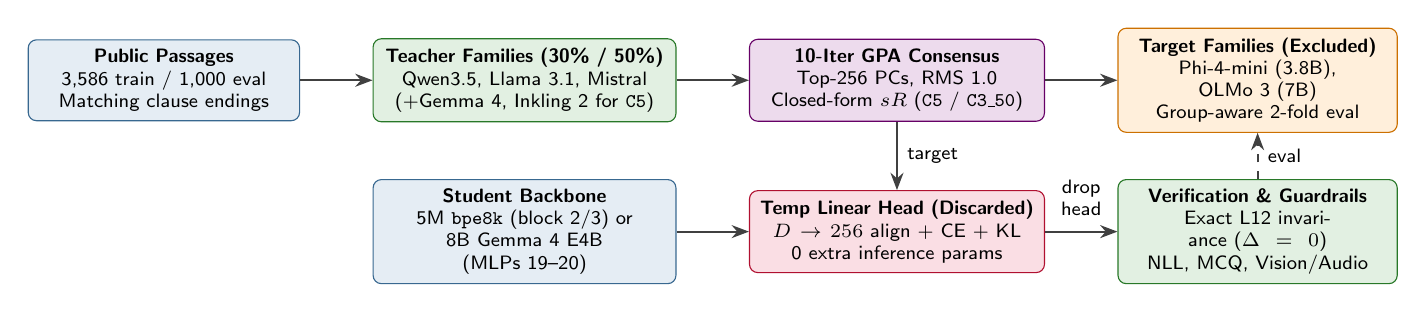
\begin{tikzpicture}[
    node distance=0.55cm and 0.92cm,
    box/.style={rectangle, rounded corners=3pt, draw=#1!80!black, fill=#1!14, text=black,
      minimum height=0.88cm, align=center, font=\sffamily\scriptsize, inner sep=3.5pt},
    arr/.style={-{Stealth[length=2.2mm]}, thick, draw=black!75}
]
  \node[box=accentblue, text width=3.2cm] (pass) {\textbf{Public Passages}\\3,586 train / 1,000 eval\\Matching clause endings};
  \node[box=accentgreen, right=of pass, text width=3.6cm] (teach) {\textbf{Teacher Families (30\% / 50\%)}\\Qwen3.5, Llama 3.1, Mistral\\(+Gemma 4, Inkling 2 for \texttt{C5})};
  \node[box=accentpurple, right=of teach, text width=3.5cm] (gpa) {\textbf{10-Iter GPA Consensus}\\Top-256 PCs, RMS 1.0\\Closed-form $s R$ (\texttt{C5} / \texttt{C3\_50})};
  \node[box=accentorange, right=of gpa, text width=3.3cm] (blind) {\textbf{Target Families (Excluded)}\\Phi-4-mini (3.8B), OLMo 3 (7B)\\Group-aware 2-fold eval};

  \node[box=accentblue, below=0.72cm of teach, text width=3.6cm] (stud) {\textbf{Student Backbone}\\5M \texttt{bpe8k} (block 2/3) or\\8B Gemma 4 E4B (MLPs 19--20)};
  \node[box=accentred, right=of stud, text width=3.5cm] (head) {\textbf{Temp Linear Head (Discarded)}\\$D \to 256$ align + CE + KL\\0 extra inference params};
  \node[box=accentgreen, right=of head, text width=3.3cm] (guard) {\textbf{Verification \& Guardrails}\\Exact L12 invariance ($\Delta=0$)\\NLL, MCQ, Vision/Audio};

  \draw[arr] (pass) -- (teach);
  \draw[arr] (teach) -- (gpa);
  \draw[arr] (gpa) -- (blind);
  \draw[arr] (gpa) -- node[right, font=\sffamily\scriptsize] {target} (head);
  \draw[arr] (stud) -- (head);
  \draw[arr] (head) -- node[above=2pt, align=center, font=\sffamily\scriptsize] {drop\\head} (guard);
  \draw[arr, dashed] (guard.north) -- node[right, font=\sffamily\scriptsize] {eval} (blind.south);
\end{tikzpicture}
\caption{Multi-family GPA denoising and zero-overhead cross-tokenizer distillation pipeline \cite{gower1975gpa,cheng2026platoskey}. Clauses align across distinct tokenizers at stripped prefix boundaries; the training-only projection head (combining alignment loss with cross-entropy [CE] and Kullback--Leibler [KL] anchoring) is discarded after optimization so deployed students carry zero added inference parameters.}
\label{fig:pipeline}
\end{figure*}

\subsection{Cross-Tokenizer Distillation (5M) and 8B Transplants}
At 5M scale, we train 24 equal-parameter (4,722,304 non-embedding / 8,916,608 total parameters, \texttt{bpe8k} vocabulary, $D=256, L=6, H=8$), equal-main-stream (100M public tokens plus 8 auxiliary passages/step, 3 seeds $\times$ 8 arms) Transformers. Supervised arms attach a temporary linear head ($256\to256$, discarded after training) at 0-indexed block 2 (33\% depth) with alignment weight \texttt{plato\_w}. Constant arms compare plain control \texttt{P0} ($\texttt{plato\_w}=0$), Gemma 4 alone \texttt{P1}, \texttt{C5} \texttt{P2}, and \texttt{C5} plus folklore \texttt{P3} ($\texttt{plato\_w}=0.25$). Annealed arms (\texttt{M0}--\texttt{M3}) decay $\texttt{plato\_w}$ from $0.25$ to $0.0$ over steps $[0.65,0.90]$, comparing instance \texttt{C5} (\texttt{M0}), leave-one-retelling-out (\texttt{LORO}) myth prototypes (\texttt{M1}), $3.5\times$ upweighted 2D $U_{\text{jung}}$ (\texttt{M2}, spanned by teacher \texttt{HOUSE} and \texttt{SELF2} contrasts), and $0.0\times$ ablated $U_{\text{jung}}$ (\texttt{M3}). A separate 1-seed, 25M-token depth-placement screen (\texttt{D0}--\texttt{D3}) tests 50\%-depth supervision at block 3 (\texttt{L3}) and dual-depth (\texttt{L2+L3}) supervision. Downstream checks measure bits per byte (bpb), syntax (\texttt{BLiMP}), commonsense (\texttt{COPA}), and multiple-choice question (\texttt{MCQ}) reading-comprehension gain (\texttt{mcq\_gain}: accuracy with passage minus without).

At 8B scale on multimodal \texttt{google/gemma-4-E4B-it} \cite{gemmateam2026gemma4}, we run two paired transplant studies with frozen Vision and Audio towers, full-rank fp32 master MLP weights cast back to bf16, and discarded linear heads ($2560\to256$; the transplant itself adds zero inference parameters):
\begin{itemize}
  \item \textbf{30\%-depth Stage A (L11--12, seed 230):} 450 paired steps ($0.25\cdot\text{CE}+1.5\cdot\text{KL}$ anchored to Base E4B, 1,350 neutral plus 450 myth draws) comparing annealed \texttt{C5} $+3.5\times U_{\text{jung}}$ ($\texttt{plato\_w}=0.40\to0$) against matched $\texttt{plato\_w}=0$ control. Gemma 4 contributes to \texttt{C5} in this earlier run.
  \item \textbf{50\%-depth Experiment 251 (L19--20, seeds 251--253):} To remove self-distillation and target the 50\%-depth stratum, we run a 4-arm paired study on neutral \texttt{gut+proc+chat} passages (450 steps, grad accum 4, AdamW $\beta=(0.9,0.95)$, MLP weight decay 0.01, 10\% linear warmup then cosine decay, grad clip 1.0, $\texttt{plato\_w}=0.40\to0$ over $[0.65,0.90]$, $0.25\cdot\text{CE}+1.5\cdot\text{KL}$, $\text{lr}_{\text{mlp}}=1.5\times10^{-5}$, $\text{lr}_{\text{head}}=10^{-3}$): unmodified \texttt{base}, matched CE+KL control \texttt{ctrl50}, 4-family \texttt{c4\_50}, and rival-only \texttt{c3\_50} (Qwen3.5 + Llama 3.1 + Mistral, zero Gemma 4). Training and extraction run through the \texttt{LivingE4B} wrapper (\texttt{aion\_8b/e4b\_living.py}) with zero-initialized Titans branches disabled during base-study extraction and enabled during multimodal sanity fixtures; the transplant itself replaces only L19--20 MLP weights, keeping layer-12 activations mathematically invariant across the 9 trained checkpoints ($\max|\Delta|=0.0$ by construction, verified on token-mean L12 states of the first 16 eval passages).
\end{itemize}
For epistemic auditing (Section~\ref{sec:epi}), \textbf{Stage B} starts from Stage A and trains four zero-initialized \texttt{Titans-Momentum} fast-weight memory branches \cite{behrouz2024titans} at layers 12, 21, 30, and 39 plus upper MLPs 40--41 for 500 steps on dialogues wrapped in our companion assistant prompt (\textit{Aion}, named after Jung's CW 9.II volume \cite{jung1968aion}, instructing concise speech and ``output ONLY \texttt{<search>query</search>}'' for live facts). Stage B is evaluated with Titans enabled from an empty state without updates (\texttt{enabled=True, state=None, update=False}).

\subsection{Narrative, Compositional, and Historical Folklore Benchmarks}
Following ARN \cite{sourati2024arn}, our 200-quartet \texttt{items3} benchmark pairs 100 myths and 100 matched technical mechanisms across four roles: \textit{anchor} (classic scene), \textit{true} (disguised modern retelling), \textit{lure} (shared nouns, unrelated plot), and \textit{foil} (broken turning point). For narrative completion, \texttt{HOUSE} contains 233 paired stories across seven categories (including 40 length-reversed \texttt{perfection} pairs) and \texttt{SELF2} adds 79 integration pairs.

To control lexical, clause-order, and static-polarity cues, we construct a sequence of exact identical-bag-of-words swap benchmarks: \texttt{bow\_swap\_60} (60 pairs), clause-order-mirrored \texttt{bow\_mirror\_120} (60 settings $\times$ 2 orders), relational \texttt{bm\_rel242} (120 pairs), valence-neutral \texttt{bm\_neut245} (120 pairs), polarity-conflict \texttt{bm\_polconf245} (120 pairs), and our main 2$\times$2 actor-intent benchmark \texttt{bm\_actor2x2\_247} (60 settings $\times$ 4 pairs = 240 pairs crossing benign versus adverse actors with mirrored clause orders, balanced across four syntactic templates: 80 \texttt{active\_and}, 56 \texttt{active\_yet}, 56 \texttt{active\_then}, 48 \texttt{two\_sentence}). In \texttt{bm\_actor2x2\_247}, an identical action flips appropriateness when the actor flips (for example, a medic versus a saboteur opening an emergency valve). This design forces all seven fitted, setting-disjoint linear lexical and polarity baselines (unigram, bigram, trigram, gap-4 skip-bigram, full-sentence polarity, predicate polarity, and local first-difference) to 50.0\%, while non-linear actor-by-polarity rules are disclosed in Section~\ref{sec:actor_depth}. We denote setting-disjoint 2-fold cross-validation (CV) by \texttt{cv2}, 2-dimensional valence projection by \texttt{VAL2} (sentiment plus outcome valence), 3-dimensional by \texttt{VAL3} (adding \texttt{HOUSE}), and 5-dimensional evaluative projection by \texttt{VAL5}.

For historical cross-cultural validation (Claim C), we audit 500 folktales drawn from Hagedorn and Dar\'anyi's open Annotated Folktales compilation (\texttt{j-hagedorn/trilogy}, \texttt{data/aft.csv}, seeded from D.~L.~Ashliman's edited and translated folktale collection and indexed to Uther's ATU catalog) \cite{hagedorn2022bearing,uther2004types}, grouped into 10 study-defined ATU division ranges. Removing 20 malformed or meta-commentary records yields 480 cleaned sentence-bounded leading excerpts ($\le 250$ words, 442 shorter than source CSV rows and 38 equal) with zero $\ge 25$-word cross-record excerpt overlaps (max 13 consecutive words overall and 7 across train/test). Before removal, pair \texttt{1244/906} shared 113 excerpt words and 448 full words, while \texttt{379/383} shared 412 full words. We also evaluate an audit-motivated 476-record framing-excluded subset (removing indices 277, 356, 383, 1390 flagged during internal review) and a 15-record debatable-provenance exclusion. Upstream licensing is mixed: \texttt{j-hagedorn/trilogy}'s \texttt{LICENSE.md} specifies CC BY-NC-SA 4.0 while its README and dataset paper cite CC BY-SA 4.0, and Ashliman's source collection carries copyright notices on specific translations and editorial text. Following the conservative boundary, our MIT repository redistributes zero text from \texttt{aft.csv}, committing only the non-text adjudication manifest (\texttt{aft\_clean248\_manifest.json}, including 500/500 per-excerpt SHA-256 digests and word counts), numeric results, and a commit-pinned fetch-and-verify script (\texttt{scripts/v6/fetch\_trilogy\_aft.py}, reproducing all 500 scored excerpts byte-for-byte). Auditing overlap against all 3,598 passages in \texttt{passages.jsonl} (\texttt{v6\_round8\_overlap\_audit.json}) confirms that Claim C's rotations used \texttt{neutral\_only=True} (2,398 neutral passages scanned, zero myth passages, 0/1,518 $\ge 12$-word overlaps with \texttt{aft.csv}, max 7 contiguous words against the 500 scored excerpts). Across all 3,598 passages including the separate Project Gutenberg \texttt{myth} pool, scored excerpts share at most 10 contiguous words, while full tales in \texttt{aft.csv} show seven $\ge 12$-word matches in the Gutenberg \texttt{myth} pool: six 21--126-word shared public-domain editions (three in the 480 set: \texttt{aft\_idx} 109, 1464, 1494, matched only outside their scored leading excerpts) plus one 14-word proverbial phrase (\texttt{myth\_0780}, \texttt{aft\_idx} 435, outside the 500 sample). Sensitivity reruns at $n=477$ and $n=473$ are reported in Section~\ref{sec:named}.

All results in Sections~\ref{sec:gpa}, \ref{sec:motifs} (Role Split), \ref{sec:jung} (Neutral Transfer through Historical Folktales), \ref{sec:distill}, and \ref{sec:8b} are backed by committed per-run JSON artifacts and sanitized runner scripts (\texttt{bench/archetypes/} and \texttt{scripts/v6/}). Our automated verifier (\texttt{scripts/verify\_repro.py}) checks every numeric cell in all verified table bodies across both this manuscript and our Markdown draft, checks core headline numbers in abstracts, conclusions, and captions, verifies all 10 multimodal fixture records, rejects any staged \texttt{aft.csv} or reconstructed tale text, inspects the arXiv archive, and runs zero-GPU unit tests plus a corruption self-test. Full GPU/MLX retraining and multi-gigabyte activation caches stay outside the repository and require open-weight downloads. The edit-position audit in Section~\ref{sec:motifs}, Section~\ref{sec:xling}, the earlier 58-label summary in Section~\ref{sec:jung}, and the Word Association summary in Section~\ref{sec:jung} summarize earlier multi-model audits whose raw captures remain external.

\section{Results}
\label{sec:results}
\subsection{Five-Family Consensus on Two Held-Out Target Families}
\label{sec:gpa}
Table~\ref{tab:gpa} and Fig.~\ref{fig:gpa} report strictly out-of-sample 2-fold transfer onto Microsoft Phi-4-mini (3.8B) and AllenAI OLMo 3 (7B), both excluded from consensus construction. Averaging five families (\texttt{C5}) outperforms every single teacher on Phi-4-mini by $+0.0523$ cosine (95\% CI $[+0.0505, +0.0541]$), $+8.3$ strict $R^2_{\text{opt}}$ points ($0.557$ vs.\ $0.474$), and $+11.3$ $R^2_{\text{frob}}$ points above Mistral 7B ($+12.4$ above Qwen3.5 9B). On OLMo 3 7B, \texttt{C5} leads every single teacher by $+0.0472$ cosine ($[+0.0458, +0.0488]$), $+7.8$ $R^2_{\text{opt}}$ points ($0.564$ vs.\ $0.486$), and $+10.4$ $R^2_{\text{frob}}$ points above Mistral 7B. Single teachers already reach 95.1\% (Llama 3.1) and 89.2\% (Mistral) tie-safe Top-1 retrieval, while \texttt{C5} reaches 95.3\% / 89.9\% and 4-family \texttt{C4} edges \texttt{C5} on every OLMo 3 metric (90.5\% Top-1, $R^2_{\text{frob}}=0.509$).

Adding looped Inkling 2 Mini lifts Phi-4-mini by $+0.0065\,[+0.0059,+0.0072]$ cosine over \texttt{C4} while keeping OLMo 3 within $-0.0007$. Refitting PCA and GPA solely on neutral pools (\texttt{gut+proc+chat}, $n=13,388$, removing all Gutenberg myths) leaves transfer nearly unchanged (Phi-4 $\cos=0.8343$, $R^2_{\text{frob}}=0.4907$, Top-1 $95.45\%$; OLMo 3 $\cos=0.7745$, $R^2_{\text{frob}}=0.5063$, Top-1 $89.89\%$). Prediction also improves on pure Gutenberg prose (\texttt{held\_gut}: \texttt{C5} $0.7534$ vs.\ best single $0.6777$ on Phi-4, and \texttt{C5} $0.7228$ / \texttt{C4} $0.7242$ vs.\ $0.6557$ on OLMo 3) and synthetic reasoning (\texttt{proc\_held}: $0.9246$ and $0.9128$), consistent with multi-family variance cancellation.

\begin{table*}[t]
\centering
\caption{Out-of-sample 2-fold transfer onto two target families excluded from GPA consensus construction (20,339 train / 3,192 eval clause points; 2,592 non-foil queries; target top-256 PCs fit on train corpus: 75.4\% var.\ Phi-4-mini, 54.7\% OLMo 3 7B). Abbreviations: Cos = cosine similarity; $R^2_{\text{opt}}$ = strict train-scalar $R^2$; $R^2_{\text{frob}}$ = norm-matched Frobenius $R^2$; T1/T5 = tie-safe Top-1/Top-5 retrieval.}
\label{tab:gpa}
\scriptsize
\setlength{\tabcolsep}{3.5pt}
\begin{tabular}{@{}lcccccc@{}}
\toprule
\textbf{Source Representation (256-dim)} & \textbf{Phi-4 Cos} & \textbf{Phi-4 $R^2_{\text{opt}}$ ($R^2_{\text{frob}}$)} & \textbf{Phi-4 T1 / T5} & \textbf{OLMo 3 Cos} & \textbf{OLMo 3 $R^2_{\text{opt}}$ ($R^2_{\text{frob}}$)} & \textbf{OLMo 3 T1 / T5} \\
\midrule
Gemma 4 E4B (Google, 30\%) & 0.6881 & 0.343 (0.180) & 91.0\% / 98.2\% & 0.6556 & 0.367 (0.225) & 86.4\% / 93.5\% \\
Llama 3.1 8B (Meta, 30\%) & 0.7666 & 0.452 (0.347) & 95.1\% / \textbf{99.4\%} & 0.7141 & 0.462 (0.368) & 88.5\% / 94.7\% \\
Mistral 7B (Mistral, 30\%) & 0.7811 & 0.474 (0.379) & 94.3\% / 99.2\% & 0.7285 & 0.486 (0.403) & 89.2\% / 94.4\% \\
Qwen3.5 9B (Alibaba, 30\%) & 0.7815 & 0.466 (0.368) & 93.6\% / 98.9\% & 0.7263 & 0.472 (0.383) & 87.4\% / 94.0\% \\
Inkling 2 Mini (Looped final) & 0.6316 & 0.268 (0.051) & 40.4\% / 68.5\% & 0.5602 & 0.236 (0.000) & 29.9\% / 57.1\% \\
\midrule
4-Family Consensus (\texttt{C4}) & 0.8273 & 0.547 (0.478) & \textbf{95.8\%} / 99.3\% & \textbf{0.7765} & \textbf{0.566} (\textbf{0.509}) & \textbf{90.5\%} / \textbf{95.0\%} \\
\textbf{5-Family Consensus (\texttt{C5})} & \textbf{0.8338} & \textbf{0.557} (\textbf{0.491}) & 95.3\% / 99.3\% & 0.7757 & 0.564 (0.506) & 89.9\% / 94.6\% \\
\bottomrule
\end{tabular}
\end{table*}

\begin{figure*}[t]
\centering
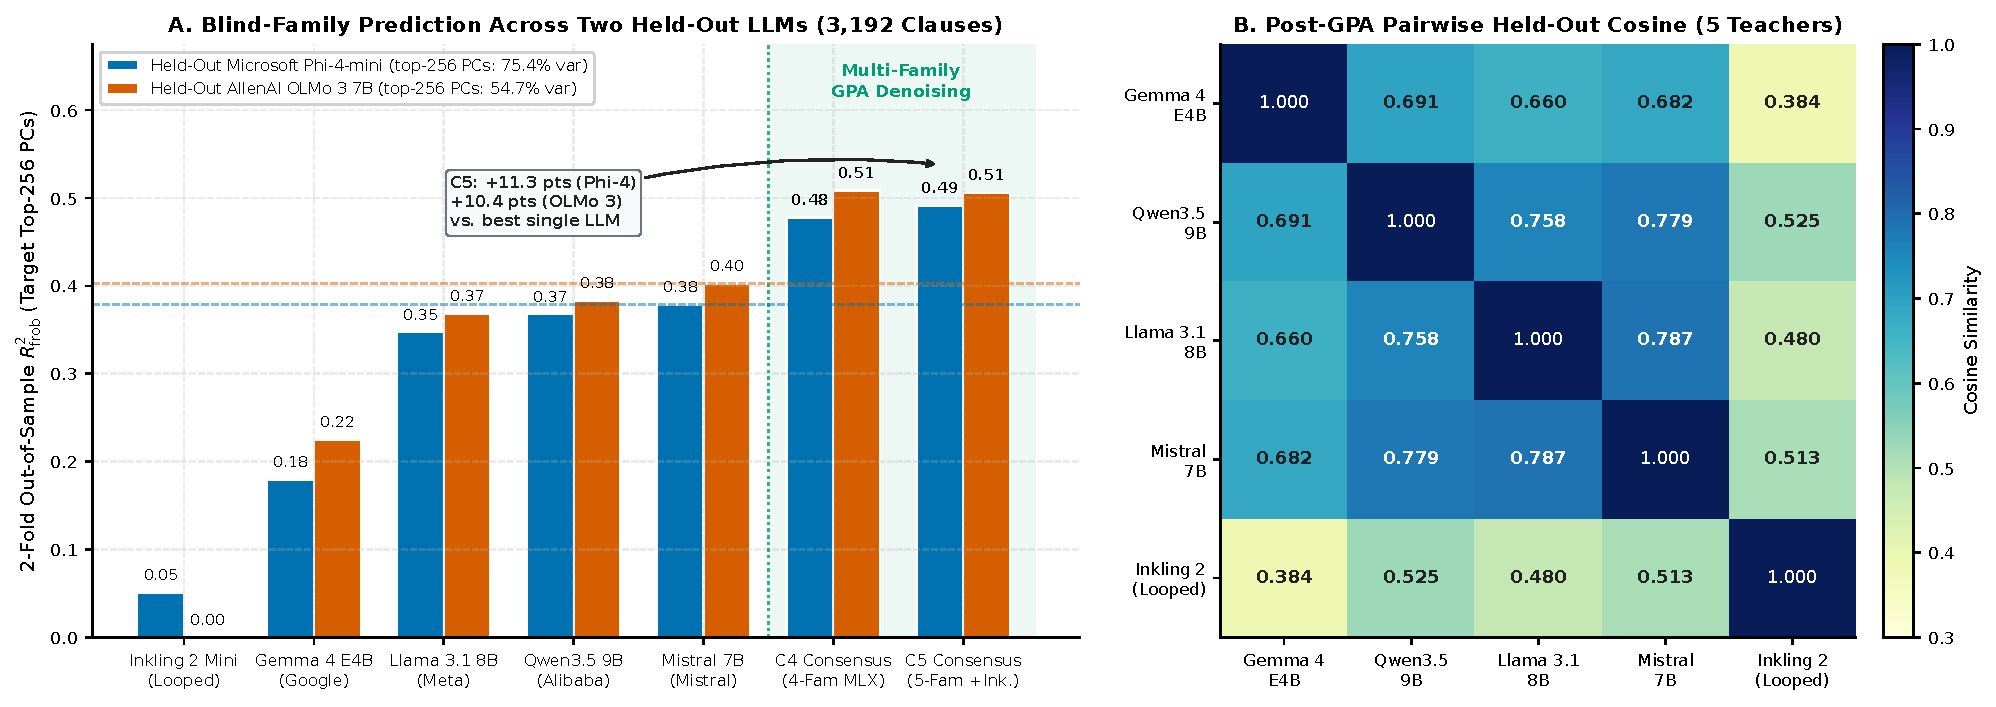
\includegraphics[width=\textwidth]{figures/fig1_platonic_consensus.pdf}
\caption{Five-family consensus evaluated on two held-out target families. \textbf{(A)} Out-of-sample 2-fold Frobenius $R^2_{\text{frob}}$ inside target top-256 PCs of Phi-4-mini and OLMo 3 7B: \texttt{C5} jumps $+10.4$ to $+11.3$ points ($+7.8$ to $+8.3$ $R^2_{\text{opt}}$) above the strongest single model (\texttt{C4}: $+9.9$ to $+10.6$). \textbf{(B)} Post-GPA pairwise held-out cosine across the five consensus teachers.}
\label{fig:gpa}
\end{figure*}

\subsection{Cultural Motifs vs.\ Disguised Plots and Edit-Position Confounding}
\label{sec:motifs}
\subsubsection{Role Split Under Myth-Pool-Excluded GPA and Proper-Name Control}
Splitting \texttt{items3} by quartet role separates cultural register from GPA basis composition (Fig.~\ref{fig:arch}A). On OLMo 3 7B, classic mythic passages align tighter than matched mechanisms even when the Gutenberg myth pool is removed from GPA (\texttt{anchor}: $+0.0512\,[+0.0332,+0.0702]$, word-matched $n=44$: $+0.0379\,[+0.0134,+0.0631]$; \texttt{lure}: $+0.0367\,[+0.0208,+0.0527]$). On Phi-4-mini, excluding the myth pool shrinks \texttt{anchor} from $+0.0103$ to $+0.0050\,[-0.0038,+0.0138]$ (n.s.) while \texttt{lure} persists at $+0.0162\,[+0.0086,+0.0243]$.

Because 77.0\% of myth \texttt{anchor} and 73.0\% of myth \texttt{lure} passages contain proper names (versus 4.0\% in mechanisms and disguised myth \texttt{true}/\texttt{foil}), we audited strictly zero-proper-name passages under myth-pool-excluded GPA (\texttt{referee\_ctrl237.json}, 2,000-draw bootstrap). The effect holds on 1 of 2 held-out models. On OLMo 3, named ($0.7131$) and name-free ($0.7071$) myth \texttt{anchor} passages sit equally above technical mechanisms ($0.6617$), giving $+0.0454\,[+0.0208,+0.0689]$ ($n=23$ vs.\ $96$) on \texttt{anchor} and $+0.0369\,[+0.0169,+0.0572]$ ($n=27$ vs.\ $96$) on \texttt{lure}. On Phi-4-mini, removing proper names reverses \texttt{anchor} ($-0.0167\,[-0.0316,-0.0009]$) and weakens \texttt{lure} ($+0.0116\,[+0.0002,+0.0231]$). Disguised modern retellings show tight nulls across both models (\texttt{true}: $-0.0005$ OLMo 3, $-0.0017$ Phi-4; \texttt{foil}: $-0.0050$, $+0.0041$, all CIs spanning zero). Surviving OLMo 3 convergence therefore tracks old-story versus technical register, whereas disguised plot structure shows no myth advantage \cite{roesler2012archetypes}.

\subsubsection{Edit-Position (\texttt{fpos}) Confounding (Earlier Audit Summary)}
Auditing earlier 8-model mean-pooled key-step RSA ($h(\text{true})-h(\text{foil})$) exposed why unadjusted RSA showed a $+0.074\,[+0.017,+0.137]$ myth lead on \texttt{items3}. Myths place their first edited word later than mechanisms (mean first-edit fraction $\texttt{fpos}=0.574$ vs.\ $0.393$, Welch $t=+6.31$, $p=1.84\times10^{-9}$). Causal mean pooling averages every post-BOS token, so early edits perturb 70--90\% of downstream states while late edits stay localized. Within mechanisms alone, \texttt{fpos} correlates with RSA at $\rho=+0.509$ ($p<10^{-7}$). Matching 1-to-1 on \texttt{fpos} (caliper 0.05, $n=64$) lowers the gap to $+0.0058\,[-0.0699,+0.0786]$ (axis-removed $-0.0008$). Minimal-edit causal LLM benchmarks using whole-sequence mean pooling must therefore match \texttt{fpos} or pool strictly after the edit token.

\subsection{Cross-Lingual Pattern Similarity and Capability Tracking}
\label{sec:xling}
Across English, Modern Greek, Japanese, and Simplified Chinese (three language families, 80 patterns, 78 with a defined same-outcome-controlled score, 5 models across three labs; committed stimuli \texttt{bench/archetypes/crosslang/}, generator \texttt{bench/archetypes/crosslang.py}, audit script \texttt{scripts/v6/crosslang\_audit.py}, output \texttt{v6\_crosslang\_audit.json}), a story's key step at 60\% depth lands closer to the same pattern in another language than to different patterns sharing outcome polarity ($+0.0789\,[+0.0630,+0.0944]$, positive across all 6 language pairs and all 5 models; edited sentences alone account for $+0.0564$ and surrounding context adds $+0.0225\,[+0.0139,+0.0305]$; myths vs.\ mechanisms $+0.0178\,[-0.0133,+0.0484]$ n.s.). On the clear sign-matched subset ($n=1,165$), cross-lingual alignment rises to $+0.1204$, whereas permuting pattern labels strictly within outcome classes gives a centered null floor of $+0.0046\,[-0.0285,+0.0427]$. Set I stories were written independently in each language (prompted not to translate) by \texttt{deepseek/deepseek-v4.1-flash-1017}, which also labeled outcome polarity. Google's Gemma 4 31B (\texttt{d31}) screened which version shows the key act (317 of 318 screened Set I stories passed; two Japanese stories failed generation, so 77 of 80 patterns are usable in all four languages; the same-outcome control needs at least three comparison patterns per side, which leaves 78: 40 myths and 38 mechanisms) and is also one of the five evaluated models, showing the largest margin ($+0.1103\,[+0.0905,+0.1308]$). Three of the five evaluated models are Google Gemma 4 checkpoints (\texttt{d31}, \texttt{e4b} $+0.0839\,[+0.0648,+0.1036]$, \texttt{a4b26} $+0.0770\,[+0.0588,+0.0958]$); the two non-Google models give $+0.0620\,[+0.0488,+0.0755]$ (Meta Llama 3.1 8B) and $+0.0615\,[+0.0465,+0.0773]$ (Alibaba Qwen3-8B). Because character 3-gram overlap ($\le 0.0001$) is near-zero by construction across distinct scripts and cannot detect conceptual overlap, and because same-pattern stories often share translation-equivalent key actions and objects, this result shows cross-lingual similarity of the key event; it does not establish a more abstract causal form. Raw activation captures (\texttt{caps\_*.npz}) are not redistributed. In an earlier 16-model capability audit (0.6B--31B), narrative pattern accuracy tracks GPQA Diamond \cite{rein2024gpqa,artificialanalysis2026evals} at Spearman $\rho=+0.943\,[+0.744,+0.996]$ ($n=14$, vs.\ $+0.868$ for parameter count; myths $+0.956$, mechanisms $+0.943$), MMLU-Pro at $+0.900$, and LiveCodeBench at $+0.839$, consistent with a dominant general capability factor \cite{ilic2023evidence}. A story-only right/wrong linear direction also predicted unseen Python bug judgment above 200 random directions in 8 of 9 models ($\rho=+0.63$, one-sided $p=0.040$).

\subsection{Completion Geometry, Compositional Readout, Named Roles, and Historical Folktales}
\label{sec:jung}
\subsubsection{Shared Center vs.\ 58 Named Labels (Earlier Audit Summary)}
Inside Gemma 4 E4B, ten narrative contrast directions share a common axis (\texttt{HOUSE}, mean pairwise cosine $+0.274$ at L25, $+0.328$ at L17). \texttt{HOUSE} aligns at $+0.164$ ($p=0.0010$) with the static SWE-smith Python bug-fix direction \cite{yang2025swesmith}, and the ten-direction span holds 4.13\% of that fix direction's squared norm ($10.6\times$ chance 0.39\%, $p=0.025$). Fixing two earlier audit bugs (centered sign-flip nulls and unconfounded live-agent fix contrast $\texttt{Q2==1}-\texttt{Q2==0}$, $n=212$) restores \texttt{SELF}/\texttt{SELF2} ($p=0.005$--$0.034$) and gives live-agent \texttt{HOUSE} cosines of $+0.091$ ($p=0.020$, L17) and $+0.175$ ($p=0.001$, L34). By contrast, 58 one-vs.-rest named labels ($N=11$--$12$ stories/label) showed no evidence of beating shuffled labels on that indirect code-fix target ($p=0.811$ static, $p=0.920$ agent; a low-power null).

\subsubsection{Zero-Shot Neutral-Text Transfer Across Six Rival Families}
Rigid Procrustes rotations fit exclusively on neutral \texttt{gut+proc+chat} text (2,394 aligned passages) transfer Gemma 4's \texttt{HOUSE} direction zero-shot into all six rival companies (Table~\ref{tab:teleport}, Fig.~\ref{fig:arch}B). Because \texttt{HOUSE} contrasts completed against degraded endings without removing outcome polarity, unigram Bag-of-Words (BoW) already reaches $95.52\%\pm0.84\%$ across 20 setting-disjoint splits ($100\%$ on \texttt{HOUSE}$\to$\texttt{SELF2}). Neutral-text neural transfer beats BoW on \textbf{20/20 splits in all six companies} (120/120 wins; 20-split means $97.42\%$--$98.93\%$, alternating 2-fold split $97.4\%$--$98.7\%$) and holds at $97.0\%$--$97.9\%$ under fold-local length residualization. It also transfers $97.5\%$--$100\%$ from \texttt{HOUSE (no-self)} to \texttt{SELF2} and denoises in \texttt{C5} ($+0.892$ Phi-4, $+0.880$ OLMo 3). Inside \texttt{C5}, $u_{\text{house,c5}}$ and $u_{\text{self2,c5}}$ are nearly collinear ($\cos=+0.9539$), and 2D $U_{\text{jung}}$ carries 1.72\% of generic \texttt{C5} variance ($2.2\times$ random 0.78\%). On \texttt{items3} plot twists, \texttt{HOUSE} fails to transfer positively on all five single-pass targets ($42.5\%$--$47.0\%$; looped Inkling 2 Mini $67.0\%$, $\cos p=0.038$), indicating that \texttt{HOUSE} tracks completion, coherence, and valence integrity rather than plot matching.

\begin{table*}[t]
\centering
\caption{Zero-shot transfer of Gemma 4's \texttt{HOUSE} (\texttt{H}) and \texttt{SELF2} directions into six rival families via neutral-only (\texttt{gut+proc+chat}) Procrustes rotations (alternating 2-fold CV shown; 20-split means $97.42\%$--$98.93\%$ vs.\ unigram BoW $95.52\%\pm0.84\%$, 120/120 wins). Columns: Cos ($p$) = direction cosine and permutation $p$; Len-Res = length-residualized accuracy; \texttt{perfection} = length-reversed subset.}
\label{tab:teleport}
\scriptsize
\setlength{\tabcolsep}{3.5pt}
\begin{tabular}{@{}lccccccc@{}}
\toprule
\textbf{Transfer (Neutral Rotation)} & \textbf{\texttt{HOUSE} Cos ($p$)} & \textbf{2-Fold Acc} & \textbf{Len-Res} & \textbf{\texttt{perfection}} & \textbf{\texttt{SELF2} Acc} & \textbf{\texttt{H}$\to$\texttt{SELF2}} & \textbf{\texttt{H}$\to$\texttt{items3}} \\
\midrule
Gemma 4 $\to$ Qwen3.5 9B (Alibaba) & +0.794 (0.001) & \textbf{98.7\%} & 97.4\% & 100.0\% & 100.0\% & \textbf{100.0\%} & 46.5\% (n.s.) \\
Gemma 4 $\to$ Llama 3.1 8B (Meta) & +0.831 (0.001) & \textbf{98.3\%} & 97.4\% & 97.5\% & 100.0\% & \textbf{100.0\%} & 47.0\% (n.s.) \\
Gemma 4 $\to$ Mistral 7B (Mistral) & +0.845 (0.001) & \textbf{97.9\%} & 97.9\% & 95.0\% & 100.0\% & \textbf{100.0\%} & 45.5\% (n.s.) \\
Gemma 4 $\to$ Inkling 2 Mini (Looped) & +0.639 (0.001) & \textbf{97.4\%} & 97.0\% & 90.0\% & 100.0\% & \textbf{98.7\%} & 67.0\% ($p=0.038$) \\
Gemma 4 $\to$ Phi-4-mini (Held-Out) & +0.797 (0.001) & \textbf{98.7\%} & 97.4\% & 97.5\% & 100.0\% & \textbf{100.0\%} & 42.5\% (below 50\%) \\
Gemma 4 $\to$ OLMo 3 7B (Held-Out) & +0.833 (0.001) & \textbf{97.9\%} & 97.0\% & 95.0\% & 100.0\% & \textbf{100.0\%} & 43.5\% (n.s.) \\
\bottomrule
\end{tabular}
\end{table*}

\begin{figure*}[t]
\centering
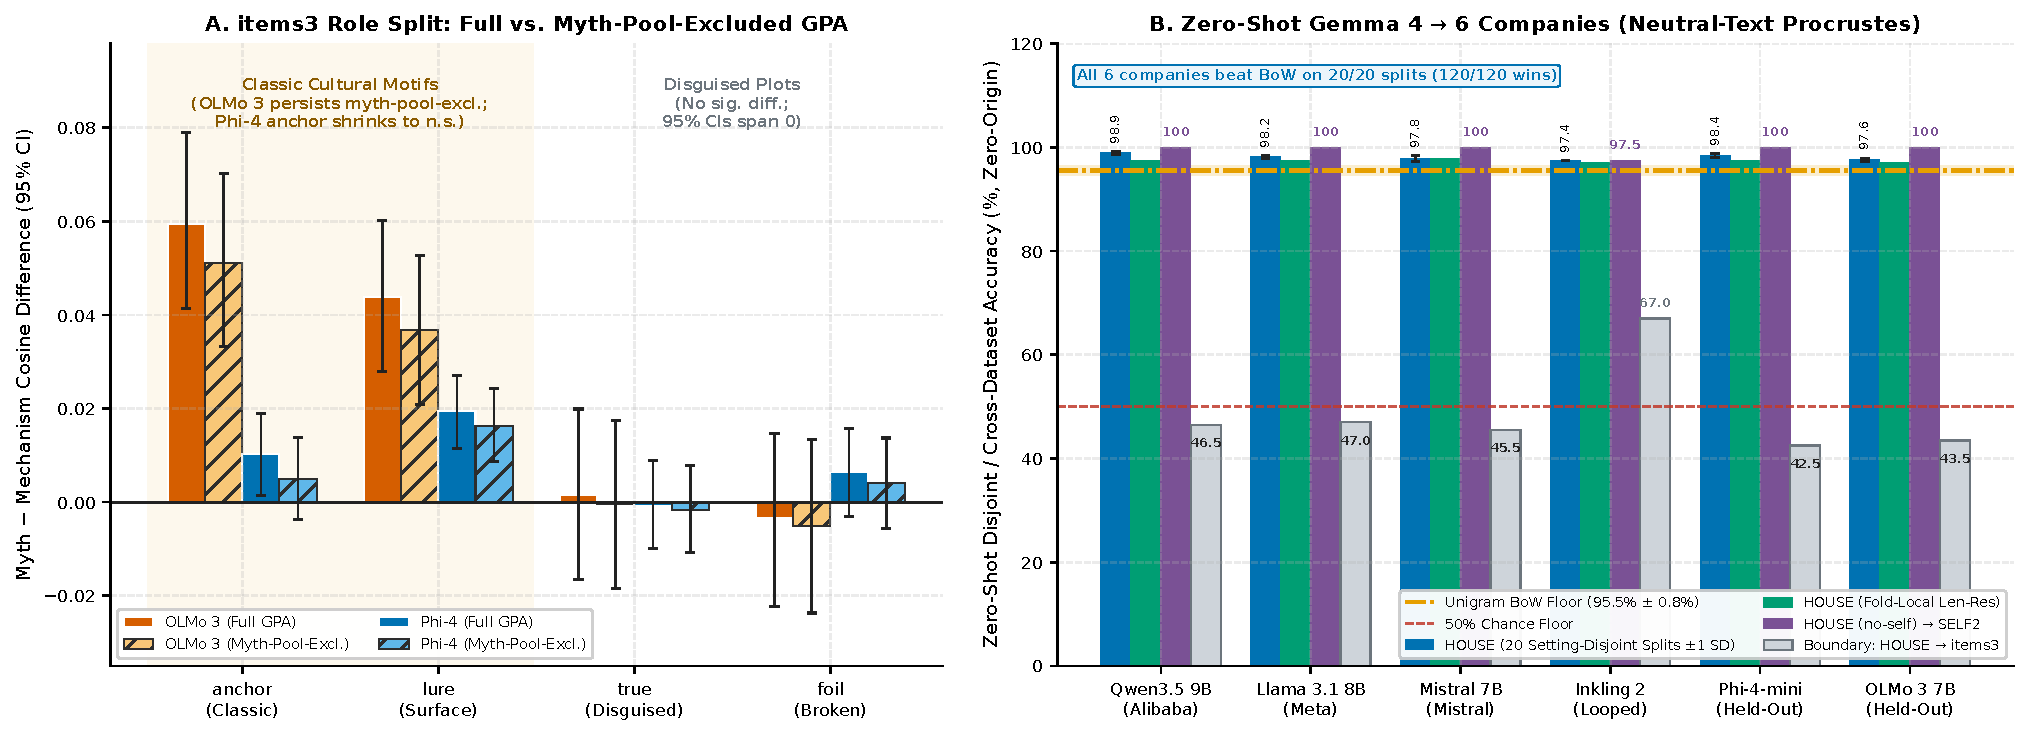
\includegraphics[width=\textwidth]{figures/fig2_archetype_audit_and_teleport.pdf}
\caption{\textbf{(A)} Role-stratified \texttt{items3} Myth minus Mechanism cosine differences (95\% CIs) under Full vs.\ Myth-Pool-Excluded GPA. \textbf{(B)} Zero-shot \texttt{HOUSE} (20 setting-disjoint splits) and \texttt{HOUSE (no-self)}$\to$\texttt{SELF2} transfer across six rival families against unigram BoW ($95.5\%\pm0.8\%$) and the \texttt{items3} boundary.}
\label{fig:arch}
\end{figure*}

\subsubsection{Valence Decomposition and Order-Mirrored Identical-BoW Swaps}
\label{sec:val}
We separate evaluative valence \cite{tigges2023linear} from structural coherence using three zero-overlap benchmarks (\texttt{valence\_ctrl234\_data.json}): 60 general sentiment pairs (\texttt{sentiment\_gen}, 100\% in all 7 models), 40 luck-only pairs (\texttt{outcome\_valence}, 100\% in all 7 models), and 60 valence-matched stories (\texttt{VM\_60}: 30 both-negative + 30 both-positive). In \texttt{C5}, \textbf{46.8\%} of \texttt{HOUSE}'s squared norm lies in $\text{span}(u_{\text{sent}}, u_{\text{outval}})$ ($\cos(u_{\text{house}}, u_{\text{sent}})=+0.6806$, $\cos(u_{\text{house}}, u_{\text{outval}})=+0.4698$, $\cos(u_{\text{sent}}, u_{\text{outval}})=+0.7568$; 37.4\%--45.6\% per model). Pure $u_{\text{sent}}$ transfers zero-shot onto \texttt{HOUSE} at $91.8\%$--$96.1\%$ (Table~\ref{tab:val}). Double-projected \texttt{HOUSE}$\perp$\texttt{VAL2} (the 53.2\% residual) still transfers at $94.7\%$--$98.1\%$ on \texttt{HOUSE} and $95.0\%$--$100.0\%$ on \texttt{VM\_60}. Lexical caveats remain on \texttt{VM\_60}, where unigram BoW reaches 100\% and \texttt{HOUSE}-trained BoW reaches $90.8\%$.

We first checked whether held-out \texttt{VAL2} projection reduces Fold-B sentiment direction transfer to chance across all 7 models ($51.7\%$--$61.7\%$, $\cos=+0.020$--$+0.042$, and \texttt{outcome\_valence} $42.5\%$--$57.5\%$). On 60 initial exact-BoW swaps (\texttt{bow\_swap\_60}, Table~\ref{tab:bswap}, unigram BoW 50.0\%, bigram 49.3\%), a $38/22$ favorable-first order skew contaminated mean pooling. Cross-order \texttt{gf}$\to$\texttt{bf} fell to $27.3\%$--$40.9\%$ on 4/6 labs, and $N=22$ balanced mean scores ($62.9\%$--$67.6\%$) were non-significant ($p=0.254$--$0.941$). Last-token pooling replaced primacy with recency ($N=22$ balanced scores $53.9\%$--$75.7\%$, only Qwen $p=0.032$).

Mirroring every setting into both clause orders (\texttt{bow\_mirror\_120}: 60 settings $\times$ 2 orders, Uni/Bi BoW 50.0\%/49.1\%, setting-disjoint 2-fold CV, setting-clustered Holm $p_{\text{holm}}$) cancels both primacy and recency (Table~\ref{tab:bmirror}). Raw zero-shot \texttt{SENT} still scores $65.0\%$--$77.5\%$ (mean) and $60.8\%$--$80.0\%$ (last) on \texttt{bm120}, while raw \texttt{HOUSE} scores $71.7\%$--$75.8\%$ (mean) and $62.5\%$--$81.7\%$ (last). After removing \texttt{VAL2}, three patterns hold. First, 2-fold \texttt{bm120}$\perp$\texttt{VAL2} clears Holm in all $6/6$ rival labs in mean pooling ($67.8\%$--$77.0\%$, $p_{\text{holm}}\le0.010$, with $42.2\%$--$58.8\%$ both-mirrors-right vs.\ 25.0\% chance and 0.0\% order-only, and $65.1\%$--$77.7\%$ $\perp$\texttt{VAL5}) and $5/6$ labs at the last token ($66.0\%$--$75.3\%$, Inkling $60.5\%$ n.s.). Second, zero-shot \texttt{HOUSE}$\perp$\texttt{VAL2}$\to$\texttt{bm120} (mean) clears Holm in $6/6$ labs ($61.7\%$--$67.5\%$, $p_{\text{holm}}\le0.014$, modest $31.7\%$--$40.0\%$ both-mirrors-right). Third, setting-clustered ordinary least squares (OLS) intercepts at equal target negative log-likelihood ($\Delta\text{NLL}=0$) stay strictly positive in $5/5$ MLX targets ($67\%$--$101\%$ of mean margin, $r=-0.010$ to $+0.277$), showing a positive fitted intercept at equal $\Delta\text{NLL}$ on those targets rather than a direct copy of final-layer output probability.

\begin{table*}[t]
\centering
\caption{Seven-company valence decomposition via neutral-only Procrustes rotations (\texttt{valence\_ctrl234.json}). \texttt{H}$\perp$\texttt{V2} projects out both sentiment ($u_{\text{sent}}$) and outcome valence ($u_{\text{outval}}$) in source and target. \texttt{VM\_60} = 60 valence-matched stories (30 both-negative / 30 both-positive; unigram BoW hits 100.0\% and \texttt{HOUSE}-trained BoW hits 90.8\%).}
\label{tab:val}
\scriptsize
\setlength{\tabcolsep}{3.5pt}
\begin{tabular}{@{}lcccc@{}}
\toprule
\textbf{Transfer (Neutral Rotation)} & \textbf{\texttt{SENT}$\to$\texttt{HOUSE}} & \textbf{\texttt{H}$\perp$\texttt{V2} 20-Split (Cos, $p$)} & \textbf{\texttt{SENT}$\to$\texttt{VM\_60} (Cos)} & \textbf{\texttt{H}$\perp$\texttt{V2}$\to$\texttt{VM\_60} (Neg/Pos, Cos, $p$)} \\
\midrule
Gemma 4 $\to$ Qwen3.5 9B (Alibaba) & 94.4\% & \textbf{98.1\%} (+0.729, 0.001) & 91.7\% (+0.241) & \textbf{100.0\%} (100\%/100\%, +0.523, 0.001) \\
Gemma 4 $\to$ Llama 3.1 8B (Meta) & 94.8\% & \textbf{96.3\%} (+0.739, 0.001) & 93.3\% (+0.262) & \textbf{98.3\%} (96.7\%/100\%, +0.504, 0.001) \\
Gemma 4 $\to$ Mistral 7B (Mistral) & 91.8\% & \textbf{96.3\%} (+0.744, 0.001) & 95.0\% (+0.278) & \textbf{100.0\%} (100\%/100\%, +0.483, 0.001) \\
Gemma 4 $\to$ Inkling 2 Mini (Looped) & 96.1\% & \textbf{95.3\%} (+0.438, 0.001) & 95.0\% (+0.291) & \textbf{95.0\%} (96.7\%/93.3\%, +0.299, 0.003) \\
Gemma 4 $\to$ Phi-4-mini (Held-Out) & 93.1\% & \textbf{94.7\%} (+0.713, 0.001) & 95.0\% (+0.259) & \textbf{100.0\%} (100\%/100\%, +0.441, 0.001) \\
Gemma 4 $\to$ OLMo 3 7B (Held-Out) & 93.1\% & \textbf{95.5\%} (+0.744, 0.001) & 95.0\% (+0.278) & \textbf{100.0\%} (100\%/100\%, +0.457, 0.001) \\
\bottomrule
\end{tabular}
\end{table*}

\begin{table*}[t]
\centering
\caption{Initial unbalanced 60-pair exact identical-BoW swap audit (\texttt{bs60} = \texttt{bow\_swap\_60}, \texttt{bow\_swap236.json}; unigram BoW 50.0\%, bigram 49.3\%). Legend: \texttt{H} = \texttt{HOUSE}; \texttt{V2}/\texttt{V5} = 2D/5D evaluative projection; 2F = setting-disjoint 2-fold CV. Order skew ($38/22$) motivated the mirrored design in Table~\ref{tab:bmirror}.}
\label{tab:bswap}
\scriptsize
\setlength{\tabcolsep}{3.0pt}
\begin{tabular}{@{}lcccccc@{}}
\toprule
\textbf{Transfer (Neutral Rotation)} & \textbf{\texttt{SENT}$\to$\texttt{bs60} ($p$)} & \textbf{\texttt{H}$\to$\texttt{bs60} ($p$)} & \textbf{\texttt{H}$\perp$\texttt{V2}$\to$\texttt{bs60} (Cos, $p$)} & \textbf{2F \texttt{bs60} Raw ($p$)} & \textbf{2F \texttt{bs60}$\perp$\texttt{V2} (Cos, $p$)} & \textbf{2F $\perp$\texttt{V5}} \\
\midrule
Gemma 4 $\to$ Qwen3.5 9B & 75.0\% (0.001) & 76.7\% (0.001) & \textbf{68.3\%} (+0.233, 0.009) & 74.9\% (0.001) & \textbf{69.9\%} (+0.303, 0.010) & 69.7\% \\
Gemma 4 $\to$ Llama 3.1 8B & 75.0\% (0.001) & 70.0\% (0.024) & 58.3\% (+0.092, 0.226 n.s.) & 77.8\% (0.016) & \textbf{72.7\%} (+0.243, 0.035) & 73.1\% \\
Gemma 4 $\to$ Mistral 7B & 75.0\% (0.001) & 80.0\% (0.001) & \textbf{61.7\%} (+0.208, 0.045) & 77.0\% (0.006) & 68.6\% (+0.218, 0.067 n.s.) & 68.3\% \\
Gemma 4 $\to$ Inkling 2 Mini & 78.3\% (0.002) & 78.3\% (0.002) & 63.3\% (+0.145, 0.090 n.s.) & 79.3\% (0.006) & \textbf{73.7\%} (+0.192, 0.027) & 72.5\% \\
Gemma 4 $\to$ Phi-4-mini & 70.0\% (0.001) & 73.3\% (0.001) & \textbf{66.7\%} (+0.175, 0.044) & 69.6\% (0.006) & \textbf{65.7\%} (+0.290, 0.027) & 65.7\% \\
Gemma 4 $\to$ OLMo 3 7B & 80.0\% (0.001) & 70.0\% (0.001) & 60.0\% (+0.123, 0.144 n.s.) & 70.9\% (0.006) & \textbf{68.7\%} (+0.236, 0.044) & 67.9\% \\
\bottomrule
\end{tabular}
\end{table*}

\begin{table*}[t]
\centering
\caption{Order-mirrored 120-pair identical-BoW swap audit and target $\Delta\text{NLL}$ control (\texttt{bow\_mirror238.json}; 60 settings $\times$ 2 mirrored orders, Uni/Bi BoW 50.0\%/49.1\%). Legend: Both = fraction getting both mirrors right (chance 25.0\%, order-only 0.0\%); $p_{\text{h}}$ = Holm-adjusted $p$; 2F = setting-disjoint 2-fold CV; \texttt{H}$\perp$\texttt{V2} = zero-shot \texttt{HOUSE} orthogonal to 2D valence; Int.\ CI = OLS intercept and 95\% CI at $\Delta\text{NLL}=0$.}
\label{tab:bmirror}
\scriptsize
\setlength{\tabcolsep}{2.0pt}
\begin{tabular}{@{}l>{\centering\arraybackslash}p{1.65cm}>{\centering\arraybackslash}p{2.50cm}>{\centering\arraybackslash}p{3.20cm}>{\centering\arraybackslash}p{3.20cm}>{\centering\arraybackslash}p{2.90cm}@{}}
\toprule
\textbf{Transfer (Mirrored 120)} & \textbf{$\Delta$NLL (Both)} & \textbf{Mean \texttt{H}$\perp$\texttt{V2} (Both, $p_{\text{h}}$)} & \textbf{Mean 2F $\perp$\texttt{V2} (Both, Cos, $p_{\text{h}}$)} & \textbf{Last 2F $\perp$\texttt{V2} (Both, Cos, $p_{\text{h}}$)} & \textbf{Mean vs.\ $\Delta$NLL ($r$, Int.\ CI)} \\
\midrule
Gemma 4 $\to$ Qwen3.5 9B & 71.7\% (51.7\%) & \textbf{67.5\%} (36.7\%, 0.006) & \textbf{70.5\%} (44.7\%, +0.395, 0.006) & \textbf{73.9\%} (51.6\%, +0.444, 0.006) & +0.261, \textbf{+0.098} [+0.055, +0.145] \\
Gemma 4 $\to$ Llama 3.1 8B & 70.8\% (50.0\%) & \textbf{65.0\%} (40.0\%, 0.008) & \textbf{77.0\%} (58.8\%, +0.392, 0.006) & \textbf{75.3\%} (54.4\%, +0.395, 0.012) & +0.277, \textbf{+0.159} [+0.097, +0.219] \\
Gemma 4 $\to$ Mistral 7B & 72.5\% (55.0\%) & \textbf{63.3\%} (33.3\%, 0.009) & \textbf{67.8\%} (42.9\%, +0.275, 0.010) & \textbf{74.4\%} (53.0\%, +0.405, 0.006) & +0.199, \textbf{+0.068} [+0.032, +0.101] \\
Gemma 4 $\to$ Inkling 2 Mini & -- & \textbf{66.7\%} (40.0\%, 0.014) & \textbf{72.8\%} (50.5\%, +0.265, 0.010) & 60.5\% (36.8\%, +0.147, 0.142 n.s.) & -- \\
Gemma 4 $\to$ Phi-4-mini & 66.7\% (41.7\%) & \textbf{65.8\%} (35.0\%, 0.006) & \textbf{68.1\%} (44.3\%, +0.357, 0.006) & \textbf{66.0\%} (39.3\%, +0.371, 0.006) & +0.180, \textbf{+0.096} [+0.048, +0.144] \\
Gemma 4 $\to$ OLMo 3 7B & 60.8\% (31.7\%) & \textbf{61.7\%} (31.7\%, 0.014) & \textbf{68.1\%} (42.2\%, +0.341, 0.006) & \textbf{70.3\%} (46.4\%, +0.335, 0.006) & $-0.010$, \textbf{+0.162} [+0.109, +0.216] \\
\bottomrule
\end{tabular}
\end{table*}

\subsubsection{\texorpdfstring{2$\times$2 Actor-Intent Readout and Five-Depth Trajectory}{2x2 Actor-Intent Readout and Five-Depth Trajectory}}
\label{sec:actor_depth}
Even on \texttt{bm120}, raw sentiment exceeds chance because every positive ending describes a favorable outcome. Our 240-pair \texttt{bm\_actor2x2\_247} benchmark removes that linear shortcut by crossing benign and adverse actors within every setting, locking all seven fitted linear lexical and polarity baselines at 50.0\% while zero-shot \texttt{zs\_sent} drops to $51.5\%$/$52.0\%$ ($98.5\%$/$98.0\%$ benign vs.\ $4.5\%$/$6.0\%$ adverse). Sweeping five depths (\texttt{d15, d30, d50, d70, d85}) across the six single-pass Transformers shows that mean-pooled linear readout strengthens from 30\% to its observed peak at 50\% depth, alongside clear pool and actor-polarity asymmetries (Table~\ref{tab:actor_depth}, Fig.~\ref{fig:actor_depth}):
\begin{itemize}
  \item \textbf{Five-depth trajectory (Claim B):} In mean-pooled cross-family \texttt{cv2}$\perp$\texttt{VAL5}, overall accuracy rises from $51.09\% \to 62.32\% \to \mathbf{73.01\%} \to 66.74\% \to 62.88\%$ (Gemma 4$\to$5) and $52.03\% \to 63.30\% \to \mathbf{73.09\%} \to 67.47\% \to 65.13\%$ (Qwen3.5$\to$5). All four mean-pool neighbor contrasts clear simultaneous cross-pool Bonferroni-8 under both percentile and reflected basic intervals (basic lower bounds $+6.37$ and $+2.19$ pp for Gemma; $+5.91$ and $+3.15$ pp for Qwen). All-four-pairs-right per setting (chance 6.25\%) peaks at 50\% depth ($0.2\% \to 9.9\% \to \mathbf{26.0\%} \to 13.2\% \to 8.9\%$ Gemma; $0.5\% \to 12.2\% \to \mathbf{28.2\%} \to 16.9\% \to 11.0\%$ Qwen). That 73\% overall average blends an easier benign half ($81.60\%$ Gemma, $87.84\%$ Qwen at \texttt{d50}) with a harder adverse half ($64.43\%$ Gemma, $58.33\%$ Qwen). On adverse actors from Gemma, mean-pool accuracy climbs from 30\% to 50\% and rebounds at 85\% ($38.6\%, 39.8\%, 64.4\%, 57.5\%, 64.2\%$). Last-token pooling is weaker and mixed: Gemma peaks at \texttt{d70} ($64.35\%$), Qwen's \texttt{d50}$-$\texttt{d30} clears percentile ($[+0.53,+11.61]$ pp) but spans zero on basic ($[-1.58,+9.50]$ pp), and \texttt{d50} last-token adverse accuracy sits below chance ($33.7\%$ Gemma, $41.2\%$ Qwen). Within-model native 6-model accuracy peaks numerically at \texttt{d50} across all five swap benchmarks (\texttt{bm\_actor2x2} $77.15\%$, 5/6 mean and 4/6 last models peaking at \texttt{d50}), clearing \texttt{d50}$-$\texttt{d30} ($[+6.68,+11.30]$ pp mean, $[+4.84,+9.63]$ pp last) while \texttt{d50}$-$\texttt{d70} basic intervals span zero ($[-0.56,+2.27]$ mean, $[-0.76,+3.37]$ last). At \texttt{d15}, all three pooled one-sided tests exceed the matched-flip refit null ($p_{\text{MC}}=1/2001$).
  \item \textbf{Zero-shot and secondary readout at \texttt{d50} (Claim A):} At \texttt{d50.last}, primary zero-shot transfer clears 0/5 Holm random-direction specificity tests ($p_{\text{holm}}=0.230$--$1.000$), \texttt{cv2} clears 2/5 on Gemma ($p_{\text{holm}}=0.010, 0.032$; others $0.120$--$0.136$), adverse accuracy sits below 50\%, and CIs against changed-span NLL span zero. In \texttt{d50.mean}, zero-shot \texttt{bm\_neut245}$\to$\texttt{actor} reaches $63.92\%$/$63.08\%$ balanced across benign ($63.3\%$/$63.2\%$) and adverse ($64.5\%$/$63.0\%$) actors, clearing 2,000-draw random specificity on 5/5 Gemma targets (Phi-4 and Mistral at $p_{\text{holm}}=0.046$) and 2/5 Qwen targets (setting \texttt{all-4} Holm: 4/5 Gemma and 3/5 Qwen, rates $3.3\%$--$13.3\%$, boundary $0.048$--$0.049$). Secondary \texttt{d50.mean} \texttt{cv2}$\perp$\texttt{VAL5} clears 5/5 Holm on item accuracy, \texttt{all-4} ($26.0\%$/$28.2\%$), and 2,000-draw random specificity, outperforming whole-sentence $\Delta$NLL by $+15.43$/$+14.09$ pp and changed-span $\Delta$NLL by $+9.60$/$+8.50$ pp (basic CIs excluding zero). On the NLL-wrong strata ($\Delta\text{NLL}\le0$), refit-in-bootstrap intervals clear 50\% on 8/10 whole and 4/10 changed cells nominally (6/10 whole and 2/10 changed under Bonferroni-20 from 2,000-resample summaries). Phi-4 whole-NLL stratum point estimates sit below 50\% ($42.72\%$/$39.95\%$, with percentile intervals spanning 50\% and Qwen$\to$Phi-4 basic $[29.43\%, 48.63\%]$ entirely below 50\%). Because single-layer steering gave a null causal effect (Exp 241, Section~\ref{sec:epi}), these results support a linear representational readout without establishing a causally localized circuit.
  \item \textbf{Incomplete projection erasure and disclosed shortcuts:} The rank-5 \texttt{VAL5} projection does not erase all evaluative sentiment: refit probes still decode Fold-B sentiment at $82.97\%$ (mean) and $82.81\%$ (last) (\texttt{v6\_erasure\_heldout\_check247.json}). Heavy Fold-A rank-40 singular value decomposition (SVD) projection leaves sentiment at $85.89\%$ while dropping held-out \texttt{cv2} from $72.58\%$ to $65.88\%$ (adverse $49.62\%$; full-corpus fit $65.13\%$ / $47.51\%$). On \texttt{bm120}$\to$\texttt{actor}, Qwen reaches $85.17\%$ ($511/600$) on benign pairs while dropping to $47.17\%$ on adverse pairs. Two explicit lexical counterexamples also beat or rival the linear probe: a frozen three-term actor-lexicon cue flips sign on $238/240$ pairs ($240/240$ adding \texttt{incorruptible}), letting text-switched $\pm\texttt{zs\_sent}$ reach $96.33\%$/$95.50\%$, and an unfitted gap-4 skip-bigram rule scores $142/240=59.17\%$ without setting-disjoint training.
\end{itemize}

\begin{table*}[t]
\centering
\caption{Five-depth trajectory (\texttt{d15}--\texttt{d85}) on \texttt{bm\_actor2x2\_247} (240 pairs; all 7 fitted linear lexical/polarity baselines $=50.0\%$; \texttt{v6\_exp247\_binding\_results.json}, \texttt{v6\_within\_model\_native\_5depth.json}, \texttt{v6\_round5\_binding\_depth\_results.json}, \texttt{v6\_round6\_final\_polish.json}). Legend: G4/Qw$\to$5 = source rotated to 5 rival families; \texttt{cv2}$\perp$\texttt{V5} = setting-disjoint 2-fold CV after rank-5 evaluative projection; Basic = reflected basic 95\% CI in percentage points (pp); Whole/Chg = pp delta vs.\ Whole-Sentence / Changed-Span target $\Delta$NLL.}
\label{tab:actor_depth}
\scriptsize
\setlength{\tabcolsep}{2.1pt}
\begin{tabular}{@{}lccccccccc@{}}
\toprule
\textbf{Protocol} & \textbf{d15} & \textbf{d30} & \textbf{d50} & \textbf{d70} & \textbf{d85} & \textbf{d50$-$d30 Basic} & \textbf{d50$-$d70 Basic} & \textbf{vs.\ Whole} & \textbf{vs.\ Chg} \\
\midrule
G4$\to$5 (mean, \texttt{cv2}$\perp$\texttt{V5}) & 51.09\% & 62.32\% & \textbf{73.01\%} & 66.74\% & 62.88\% & $[+6.37,+14.37]$ & $[+2.19,+9.61]$ & $+15.43$ & $+9.60$ \\
Qw$\to$5 (mean, \texttt{cv2}$\perp$\texttt{V5}) & 52.03\% & 63.30\% & \textbf{73.09\%} & 67.47\% & 65.13\% & $[+5.91,+12.88]$ & $[+3.15,+8.30]$ & $+14.09$ & $+8.50$ \\
G4$\to$5 (last, \texttt{cv2}$\perp$\texttt{V5}) & 50.52\% & 60.27\% & 61.60\% & \textbf{64.35\%} & 63.30\% & $[-4.32,+4.83]$ & $[-9.29,+1.01]$ & $+4.02$ & $-1.82$ \\
Qw$\to$5 (last, \texttt{cv2}$\perp$\texttt{V5}) & 50.41\% & 60.08\% & \textbf{65.09\%} & 59.91\% & 59.24\% & $[-1.58,+9.50]$ & $[+1.79,+8.34]$ & $+6.09$ & $+0.51$ \\
Native Mean (6-Mod) & 53.58\% & 68.02\% & \textbf{77.15\%} & 75.60\% & 73.35\% & $[+6.68,+11.30]^\dagger$ & $[-0.56,+2.27]^\dagger$ & -- & -- \\
Native Last (6-Mod) & 51.55\% & 63.16\% & \textbf{70.48\%} & 68.98\% & 68.67\% & $[+4.84,+9.63]^\dagger$ & $[-0.76,+3.37]^\dagger$ & -- & -- \\
\bottomrule
\multicolumn{10}{@{}l@{}}{\scriptsize $^\dagger$Cross-family CIs (pp) are Bonferroni-8 across both pools; native CIs are Bonferroni-2. Qw last \texttt{d50$-$d30} clears percentile ($[+0.53,+11.61]$) only.}
\end{tabular}
\end{table*}

\begin{figure*}[t]
\centering
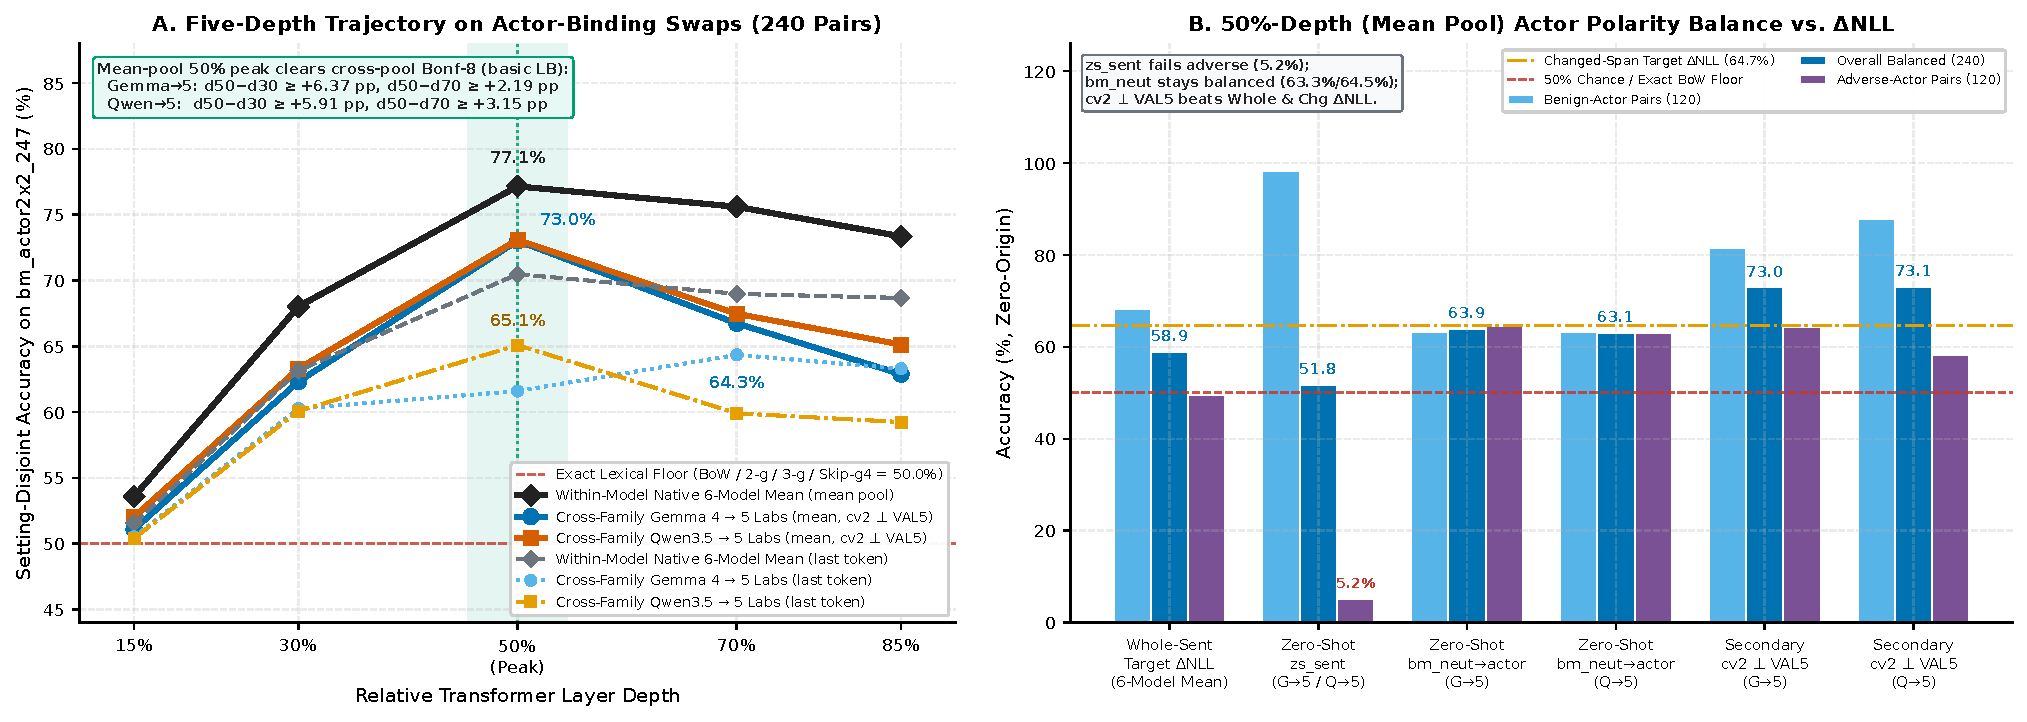
\includegraphics[width=\textwidth]{figures/fig7_depth_and_actor_binding.pdf}
\caption{\textbf{(A)} Five-depth trajectory on \texttt{bm\_actor2x2\_247} (240 pairs; 7 fitted linear lexical/polarity baselines at 50.0\%): mean-pooled cross-family readout peaks at 50\% depth while last-token curves are weaker. \textbf{(B)} 50\%-depth benign-vs.-adverse balance contrasting raw sentiment collapse (5.2\% adverse) against balanced zero-shot \texttt{bm\_neut}$\to$\texttt{actor} and \texttt{cv2}$\perp$\texttt{VAL5}.}
\label{fig:actor_depth}
\end{figure*}

\subsubsection{Study-Selected Jung-Inspired Roles, Workplace Controls, and Historical ATU Folktales}
\label{sec:named}
We authored 320 setting-balanced modern micro-stories covering eight study-selected Jung-inspired narrative roles (\textit{Hero, Shadow, Trickster, Wise\_Old\_Man, Great\_Mother, Persona, Anima\_Animus, Threshold\_Guardian}, 40 settings $\times$ 8 roles, zero role-name leaks; \textit{Threshold Guardian} derives from Campbell/Vogler storytelling typologies \cite{vogler2007writers}, \textit{Persona} and \textit{Anima/Animus} are psychic structures in Jung rather than story roles, and the \textit{Self} is omitted). We paired them against eight ordinary workplace roles (\textit{Auditor, Repair\_Tech, Negotiator, Scheduler, Trainer, Supplier, Journalist, Archivist}) in the same 40 settings (Tables~\ref{tab:named}--\ref{tab:nonjung}) and eight everyday family roles (\texttt{family\_roles239\_data.json}). All 48/48 role$\times$lab cells clear $p=0.001$ on both sets, yet \textbf{ordinary workplace roles transfer higher} ($94.3\%$--$98.1\%$ raw / $93.4\%$--$98.5\%$ $\perp$\texttt{VAL3}) than Jung-inspired roles ($85.9\%$--$92.7\%$ raw / $86.7\%$--$91.4\%$ $\perp$\texttt{VAL3}). Workplace labels also have higher lexical separability (term-frequency inverse-document-frequency [TF-IDF] Ridge $99.4\%$ vs.\ $89.1\%$). Neither set compresses effective participation rank (\texttt{PR}, defined as $(\sum\lambda_i)^2/\sum\lambda_i^2$) significantly below 500 within-setting label shuffles in \texttt{C5} (Jung $5.009$ vs.\ null $5.533$, $p=0.116$; Workplace $4.379$ vs.\ null $5.051$, $p=0.108$).

\begin{table*}[t]
\centering
\caption{Zero-shot neutral-text transfer of 8 study-selected Jung-inspired narrative roles across 6 rival families (\texttt{named\_arch235.json}, 20 setting-disjoint splits; chance 12.5\%; BoW 80.6\% / 0.958; TF-IDF Ridge [TFR] 89.1\% / 0.984; all 48/48 cells $p=0.001$). Columns: T1 = Top-1 accuracy; AUROC = macro area under receiver operating characteristic; $\perp$\texttt{V3} = 3D valence/coherence projection; Len-Res = length-residualized; Within-Set = within-setting accuracy.}
\label{tab:named}
\scriptsize
\setlength{\tabcolsep}{3.5pt}
\begin{tabular}{@{}lcccccc@{}}
\toprule
\textbf{Transfer (Neutral Rotation)} & \textbf{Raw Top-1 (vs.\ TFR)} & \textbf{$\perp$\texttt{VAL3} Top-1 (vs.\ TFR)} & \textbf{Raw AUROC} & \textbf{$\perp$\texttt{V3} AUROC} & \textbf{Len-Res T1} & \textbf{Within-Set T1} \\
\midrule
Gemma 4 $\to$ Qwen3.5 9B & \textbf{89.9\%} (11/20) & \textbf{89.4\%} (9/20) & 0.972 & 0.965 & 87.8\% & 90.5\% \\
Gemma 4 $\to$ Llama 3.1 8B & \textbf{92.7\%} (20/20) & \textbf{91.4\%} (19/20) & 0.976 & 0.971 & 91.2\% & 90.2\% \\
Gemma 4 $\to$ Mistral 7B & \textbf{92.3\%} (20/20) & \textbf{91.1\%} (15/20) & 0.974 & 0.968 & 90.0\% & 91.2\% \\
Gemma 4 $\to$ Inkling 2 Mini & 85.9\% (0/20) & 86.7\% (0/20) & 0.967 & 0.964 & 84.0\% & 90.0\% \\
Gemma 4 $\to$ Phi-4-mini & 88.5\% (8/20) & 87.5\% (2/20) & 0.965 & 0.959 & 87.4\% & 87.4\% \\
Gemma 4 $\to$ OLMo 3 7B & \textbf{91.9\%} (19/20) & \textbf{90.3\%} (14/20) & 0.973 & 0.966 & 89.2\% & 90.6\% \\
\bottomrule
\end{tabular}
\end{table*}

\begin{table*}[t]
\centering
\caption{Direct non-Jungian control (\texttt{referee\_ctrl237.json}): 8 everyday workplace roles in the exact same 40 settings (BoW 94.9\% / 0.995; TF-IDF Ridge [TFR] 99.4\% / 1.000). All 48/48 cells $p=0.001$; \texttt{C5} \texttt{PR} $=4.38$/$4.74$ vs.\ Jung's $5.01$/$5.06$ (both n.s., $p=0.108$/$0.116$). Legend matches Table~\ref{tab:named}.}
\label{tab:nonjung}
\scriptsize
\setlength{\tabcolsep}{3.5pt}
\begin{tabular}{@{}lcccccc@{}}
\toprule
\textbf{Transfer (Non-Jungian Control)} & \textbf{Raw Top-1 (BoW / TFR)} & \textbf{$\perp$\texttt{VAL3} Top-1 (TFR)} & \textbf{Raw AUROC} & \textbf{$\perp$\texttt{V3} AUROC} & \textbf{Len-Res T1} & \textbf{Within-Set T1} \\
\midrule
Gemma 4 $\to$ Qwen3.5 9B & \textbf{97.2\%} (19/20 / 0/20) & \textbf{97.2\%} (0/20) & 0.992 & 0.993 & 94.2\% & 97.2\% \\
Gemma 4 $\to$ Llama 3.1 8B & \textbf{97.8\%} (20/20 / 0/20) & \textbf{98.4\%} (1/20) & 0.995 & 0.996 & 95.4\% & 98.7\% \\
Gemma 4 $\to$ Mistral 7B & \textbf{97.9\%} (20/20 / 0/20) & \textbf{97.8\%} (0/20) & 0.992 & 0.994 & 97.2\% & 98.0\% \\
Gemma 4 $\to$ Inkling 2 Mini & 94.3\% (3/20 / 0/20) & 93.4\% (0/20) & 0.984 & 0.987 & 92.1\% & 96.1\% \\
Gemma 4 $\to$ Phi-4-mini & \textbf{98.1\%} (20/20 / 0/20) & \textbf{98.5\%} (0/20) & 0.990 & 0.992 & 95.4\% & 96.0\% \\
Gemma 4 $\to$ OLMo 3 7B & \textbf{97.5\%} (20/20 / 0/20) & \textbf{97.6\%} (0/20) & 0.992 & 0.993 & 95.1\% & 97.1\% \\
\bottomrule
\end{tabular}
\end{table*}

Testing whether our modern micro-story subspaces match real historical folktales, we projected 480 cleaned ATU excerpts (plus the audit-motivated 476-record framing-excluded subset) through neutral-only (\texttt{gut+proc+chat}) \texttt{C5} rotations (Tables~\ref{tab:folklore}--\ref{tab:folk_transfer}, Fig.~\ref{fig:folklore}, Claim C). We score each 7-dimensional basis by $v_{\text{dir}}$, the equal-class mean squared directional projection of unit one-versus-rest ATU division directions onto that basis. \textbf{Our primary finding is negative regarding uniquely Jungian privilege:} five predicted Jung-to-ATU diagonal pairings fail ($\text{mean }\cos=-0.1064$, permutation $p=0.952$, and 476-record $-0.110$, $p=0.957$), type-preserving effective rank is null ($5.539$ vs.\ $5.835$, $p=0.277$), and unlabeled PCA fitted to the same Jung corpus achieves a higher $v_{\text{dir}}$ than labeled Jungian centroids. Under fixed-source division-stratified whole-ATU-type bootstrapping, setting-centered \texttt{PCA7\_jung\_setcent} ($0.15729$ on 480, $0.15547$ on 476) outperforms \texttt{Q\_jung7} ($0.13803$ / $0.13719$) under both percentile and basic intervals (Holm-7 $p=0.007$/$0.008$ on 480 and $0.007$/$0.012$ on 476). Raw unlabeled \texttt{PCA7\_jung} ($0.16013$ / $0.15841$) clears fixed-source percentile Holm-7 ($0.032$/$0.034$) and crosses $0.05$ on basic ($0.088$/$0.122$). Under joint source--target resampling on 480 records, both contrasts span zero on basic intervals: raw \texttt{PCA7\_unlabeled}$-$\texttt{Q\_jung7} is $[-0.00764, +0.04965]$ (percentile $[-0.00544, +0.05185]$), while \texttt{PCA7\_setcent}$-$\texttt{Q\_jung7} clears percentile ($[+0.00519, +0.03967]$) and spans zero on basic ($[-0.00116, +0.03332]$).

Against within-setting shuffled labels, \texttt{Q\_jung7} shows a modest positive lift ($0.13803$ vs.\ 200-draw mean $0.09631$, 10,000-draw $138/10000$, $p_{\text{upper}}=0.0139$, mixed-draw Holm-3 $p=0.0417$; 476-record $0.13719$ vs.\ $0.09600$, 10k $147/10000$, $p_{\text{upper}}=0.0148$, Holm-3 $0.0444$). On ATU $v_{\text{dir}}$, both Jung ($0.13803$) and Family ($0.11332$) bases outscore Workplace bases ($0.07300$ / $0.08913$, \texttt{Q\_jung7}$-$\texttt{Q\_jobs7} Holm-7 $0.007$/$0.007$), while Jung shows no reliable advantage over Family ($p_{\text{holm}}=0.304$/$0.088$). Rerunning the seven basis scores, all seven fixed-source Holm-7 contrasts, and the 10k Jung / 200-draw Family and Workplace shuffles after removing the three records whose unscored full tales match Gutenberg editions (\texttt{v6\_round8\_overlap\_audit.json}, $n=477$ and $n=473$) preserves those main structural outcomes: at $n=477$, \texttt{Q\_jung7} is $0.13772$ (10k $134/10000$, $p_{\text{upper}}=0.0135$, Holm-3 $0.0405$), \texttt{PCA7\_setcent} ($0.15685$) beats \texttt{Q\_jung7} (nominal $p=0.001$/$0.002$, Holm-7 $0.007$/$0.008$), and \texttt{Q\_jung7} beats \texttt{Q\_jobs7} ($0.07064$, Holm-7 $0.007$/$0.007$); at $n=473$, \texttt{Q\_jung7} is $0.13687$ (10k $137/10000$, $p_{\text{upper}}=0.0138$, Holm-3 $0.0414$), \texttt{PCA7\_setcent} ($0.15498$) beats \texttt{Q\_jung7} (nominal $0.001$/$0.003$, Holm-7 $0.007$/$0.012$), and \texttt{Q\_jung7} beats \texttt{Q\_jobs7} ($0.07195$, Holm-7 $0.007$/$0.007$). One secondary contrast weakens: raw \texttt{PCA7\_jung}$-$\texttt{Q\_jung7} moves to nominal $p=0.029$/$0.070$ (Holm-7 $0.058$/$0.118$) at $n=477$ and $0.027$/$0.091$ (Holm-7 $0.054$/$0.114$) at $n=473$.

In cross-cultural Western$\to$Non-Western ATU classification (strictly ATU-type-disjoint English-rendered excerpts, 20,000-draw shared bootstraps, Table~\ref{tab:folk_transfer}), neural \texttt{C5}$\perp$\texttt{VAL3} clears chance on $8/8$ model$\times$metric cells across all four splits (Holm-8 $\le 0.008$). Against all three lexical baselines (pooled true-9 macro AUROC $0.4884$--$0.5028$ across all four splits, and $0.4931$--$0.5028$ across the two main splits), primary 10-bin transfer clears only $2/8$ cells on 480 ($n_{\text{train}}/n_{\text{test}}=121/137$) and 476 ($120/137$, with $2/8$ on 480-excl-15 and $1/8$ on 476-excl-15) because Western training over-represents Stupid Ogre tales, leaving six of ten bins with $\le 2$ hits. In sensitivity analyses dropping that 2-item test bin, true 9-class refits ($n_{\text{train}}/n_{\text{test}}=84/135$ on 480, $83/135$ on 476, $85/120$ on 480-excl-15, $84/120$ on 476-excl-15, majority-class oracle $41/135=30.4\%$) yield neural Top-1 of $24.4\%$--$35.6\%$ (Phi-4 below oracle, Gemma at oracle), macro AUROC $0.597$--$0.626$ (480) / $0.597$--$0.623$ (476), and $6/8$ (480, three cells tied at $0.047$) or $5/8$ (476 and 476-excl-15) Holm-8 passes over lexical baselines. Under joint-16 multiplicity covering 10-bin plus 9-bin 9-way evaluation (excluding the separate true-9 refit), only $3/16$ (480), $1/16$ (476), and $2/16$ (476-excl-15) cells pass.

\begin{table*}[t]
\centering
\caption{Internally specified historical ATU folktale structural audit on 480 cleaned excerpts and 476 audit-motivated framing-excluded excerpts from Hagedorn and Dar\'anyi \cite{hagedorn2022bearing,uther2004types} (\texttt{v6\_round4\_folklore\_results.json}, \texttt{v6\_round6\_final\_polish.json}, \texttt{v6\_round7\_claim\_c\_seal.json}). Legend: $v_{\text{dir}}$ = equal-class mean squared directional projection of unit one-vs.-rest ATU directions onto each 7D basis in neutral-only \texttt{C5}; 200-Shuf Mean = mean of 200 within-setting label shuffles; Shuf H3 = Holm-3 across Jung/Family/Workplace (10,000 draws for Jung, 200 draws for Family/Workplace); Holm-7 = fixed-source division-stratified whole-type bootstrap (Pct/Bas = percentile / reflected basic).}
\label{tab:folklore}
\scriptsize
\setlength{\tabcolsep}{3.0pt}
\begin{tabular}{@{}lccccc@{}}
\toprule
\textbf{Subspace Basis (7D in \texttt{C5})} & \textbf{$v_{\text{dir}}$ (480)} & \textbf{$v_{\text{dir}}$ (476)} & \textbf{200-Shuf Mean (480/476)} & \textbf{Shuf H3 (480/476)} & \textbf{vs.\ \texttt{Q\_jung7} Holm-7 (Pct/Bas)} \\
\midrule
\texttt{PCA7\_jung\_unlabeled} & \textbf{0.16013} & \textbf{0.15841} & -- & -- & 0.032 / 0.088 (476: 0.034 / 0.122) \\
\texttt{PCA7\_jung\_setcent} & 0.15729 & 0.15547 & -- & -- & \textbf{0.007 / 0.008} (476: \textbf{0.007 / 0.012}) \\
\texttt{PCA7\_fam\_unlabeled} & 0.13931 & 0.13810 & -- & -- & -- \\
\textbf{\texttt{Q\_jung7\_labeled}} & 0.13803 & 0.13719 & 0.09631 / 0.09600 & \textbf{0.0417 / 0.0444}$^*$ & Reference \\
\texttt{Q\_fam7\_labeled} & 0.11332 & 0.11223 & 0.10072 / 0.10063 & 0.547 / 0.567 n.s. & 0.304 / 0.088 (476: 0.296 / 0.122 n.s.) \\
\texttt{PCA7\_jobs\_unlabeled} & 0.08913 & 0.08916 & -- & -- & vs.\ \texttt{PCA7\_jung}: \textbf{0.007 / 0.007} \\
\texttt{Q\_jobs7\_labeled} & 0.07300 & 0.07434 & 0.06907 / 0.06952 & 0.547 / 0.567 n.s. & \textbf{0.007 / 0.007} (both splits) \\
\bottomrule
\multicolumn{6}{@{}p{15.8cm}@{}}{\scriptsize $^*$10,000-draw Jung shuffle ($138/10000$ on 480, $147/10000$ on 476); Family and Workplace use 200-draw shuffles. Five predicted Jung--ATU diagonal pairs fail ($\cos=-0.106, p=0.952$).}
\end{tabular}
\end{table*}

\begin{table*}[t]
\centering
\caption{Western$\to$Non-Western strictly ATU-type-disjoint true 9-class refit sensitivity analysis across four splits (\texttt{v6\_round6\_final\_polish.json}, \texttt{v6\_round7\_claim\_c\_seal.json}). Legend: $n_{\text{tr}}/n_{\text{te}}$ = fitted train / held-out test tale counts (480 test majority oracle = 41/135 = 30.4\%); Lex = BoW, TF-IDF centroid, and TF-IDF Ridge range; Neural = 4 models in \texttt{C5}$\perp$\texttt{VAL3} (Phi-4, Gemma 4, OLMo 3, Qwen3.5); H8 = 20k shared-bootstrap Holm-8 pass count.}
\label{tab:folk_transfer}
\scriptsize
\setlength{\tabcolsep}{3.0pt}
\begin{tabular}{@{}lcccccc@{}}
\toprule
\textbf{True-9 Refit Split} & \textbf{$n_{\text{tr}}/n_{\text{te}}$} & \textbf{Lex AUROC} & \textbf{Neural AUROC} & \textbf{Neural Bal.\ Acc.} & \textbf{vs.\ Lex H8} & \textbf{vs.\ Chance H8} \\
\midrule
480 Main & 84 / 135 & 0.4968--0.5028 & 0.5970--0.6258 & 21.98\%--26.93\% & 6/8 & \textbf{8/8} ($\le 0.006$) \\
476 Main (framing excl.) & 83 / 135 & 0.4931--0.5005 & 0.5965--0.6226 & 21.71\%--28.18\% & 5/8 & \textbf{8/8} ($\le 0.006$) \\
480 Excl-15 (debatable prov.) & 85 / 120 & 0.4905--0.4949 & 0.5957--0.6271 & 22.73\%--29.20\% & 6/8 & \textbf{8/8} ($\le 0.008$) \\
476 Excl-15 & 84 / 120 & 0.4884--0.4938 & 0.5946--0.6240 & 22.73\%--28.28\% & 5/8 & \textbf{8/8} ($\le 0.008$) \\
\bottomrule
\end{tabular}
\end{table*}

\begin{figure*}[t]
\centering
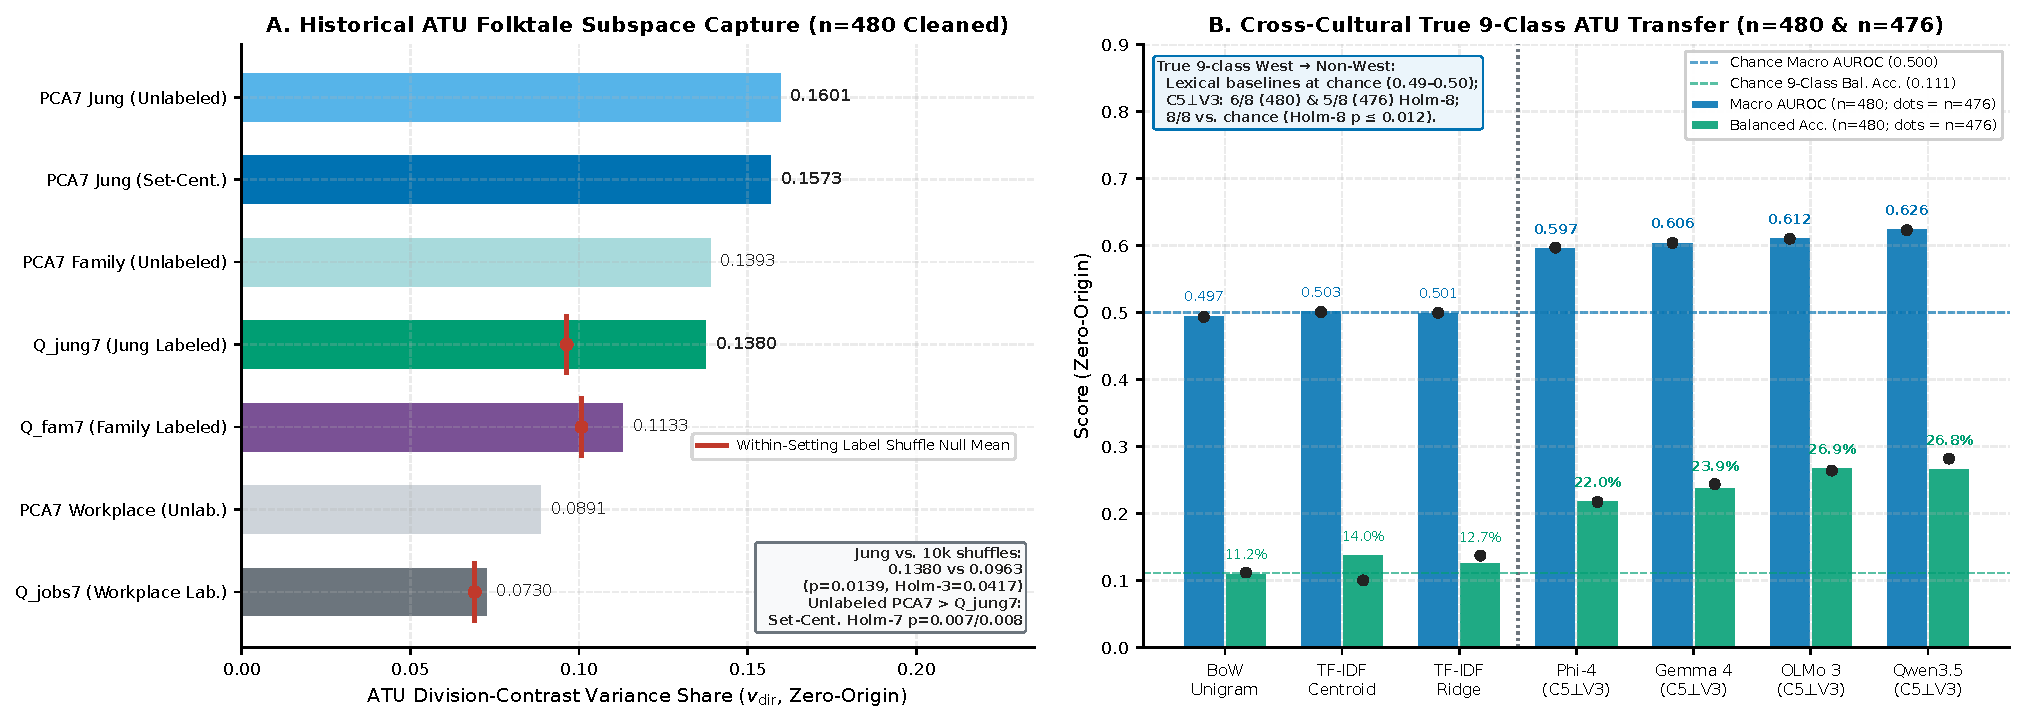
\includegraphics[width=\textwidth]{figures/fig9_historical_folklore_audit.pdf}
\caption{\textbf{(A)} Seven-basis mean squared directional projection ($v_{\text{dir}}$) on 480 cleaned historical folktales from Hagedorn and Dar\'anyi \cite{hagedorn2022bearing,uther2004types} with 200-draw shuffle null means (red markers): predicted Jung--ATU pairings fail ($\cos=-0.106, p=0.952$) and unlabeled PCA scores higher than labeled Jungian axes, though \texttt{Q\_jung7} modestly exceeds 10k shuffles ($p_{\text{holm}}=0.0417$). \textbf{(B)} True 9-class Western$\to$Non-Western refit sensitivity analysis ($n_{\text{tr}}/n_{\text{te}}=84/135$ bars, $83/135$ dots; majority oracle 30.4\%).}
\label{fig:folklore}
\end{figure*}

\subsubsection{Word Association and Mid-Depth Placement (Earlier Audit Summary)}
Across 17 open models on the 99 unique cues from Jung's 1904--1909 Word Association list \cite{jung1973experimental}, token entropy disturbance correlates across labs ($+0.109$ pairs, $+0.231$ company-averaged). Yet LLMs show no selective disturbance on clinical words ($-0.098\,[-0.207,+0.011]$), tracking abstractness ($r=-0.333$) rather than DeepSeek model-rated word arousal ($+0.027$), and show zero detected perseveration ($0/17$ models in that stateless multi-turn assay). A legacy semantic-clustering signal ($13/17$) retired as a literal ``\texttt{to }'' verb-prefix artifact ($3/17$ corrected), and feed-forward network (FFN) layers expand rather than contract perturbations across depth ($+0.023$ from 20\% to 80\% depth). A 3-seed JEPA placement ablation showed top-layer invariance harms causal-foil discrimination (\texttt{TF} $-0.074\,[-0.136,-0.011]$), whereas mid-depth invariance removes that penalty ($-0.012$) while lifting cross-view retrieval ($0.870$ vs.\ $0.789$) \cite{huang2025llmjepa,cheng2026platoskey}.

\subsection{Cross-Tokenizer Distillation at 5M Scale and Cross-Setting Retrieval}
\label{sec:distill}
\subsubsection{199-Family Cross-Setting LORO Retrieval vs.\ Strict-LQO TF-IDF}
Across 975 verified modern workplace stories spanning 199 pattern families ($182\times5, 14\times4, 3\times3$; four cumulative beats \texttt{beat\_0}--\texttt{beat\_3}), Table~\ref{tab:loro} and Fig.~\ref{fig:loro} compare strict leave-one-retelling-out (\texttt{LORO}) retrieval in frozen \texttt{C5} against single held-out models and strictly leave-query-out unigram TF-IDF. Frozen \texttt{C5} beats both single models and TF-IDF on opening beats (\texttt{beat\_0}: $12.4\%$ vs.\ $5.5\%$, $2.24\times$; \texttt{beat\_1}: $40.6\%$/$63.5\%$ Top-5 vs.\ $34.7\%$/$55.5\%$). Once passages lengthen across \texttt{beat\_2}--\texttt{beat\_3}, cumulative vocabulary lets TF-IDF overtake mid-layer vectors ($51.4\%$ and $57.9\%$, exact $565/975$). On third-party external systems-archetype texts (Exp 243, Section~\ref{sec:epi}), however, neural retrieval trailed unigram BoW even at early summary length, bounding this early-arc advantage to our workplace retelling corpus.

\begin{table}[t]
\centering
\caption{Strict leave-query-out (LQO) LORO retrieval across 199 pattern families (975 stories; chance 0.50\% T1 / 2.51\% T5) vs.\ strict-LQO unigram TF-IDF. Legend: T1/T5 = Top-1 / Top-5 accuracy (\%); \texttt{beat\_0}--\texttt{beat\_3} = cumulative story quarters.}
\label{tab:loro}
\scriptsize
\setlength{\tabcolsep}{3.5pt}
\begin{tabular}{@{}lcccc@{}}
\toprule
\textbf{Beat} & \textbf{\texttt{C5} T1/T5} & \textbf{Phi-4 T1/T5} & \textbf{OLMo 3 T1/T5} & \textbf{TF-IDF T1/T5} \\
\midrule
\texttt{beat\_0} & \textbf{12.4 / 24.8} & 7.9 / 18.3 & 7.7 / 17.4 & 5.5 / 13.6 \\
\texttt{beat\_1} & \textbf{40.6 / 63.5} & 32.8 / 54.9 & 29.3 / 47.6 & 34.7 / 55.5 \\
\texttt{beat\_2} & 36.7 / 62.1 & 40.9 / 62.8 & 28.3 / 46.6 & \textbf{51.4 / 71.1} \\
\texttt{beat\_3} & 31.5 / 58.2 & 32.8 / 59.5 & 22.7 / 42.1 & \textbf{57.9 / 78.8} \\
\bottomrule
\end{tabular}
\end{table}

\begin{figure*}[t]
\centering
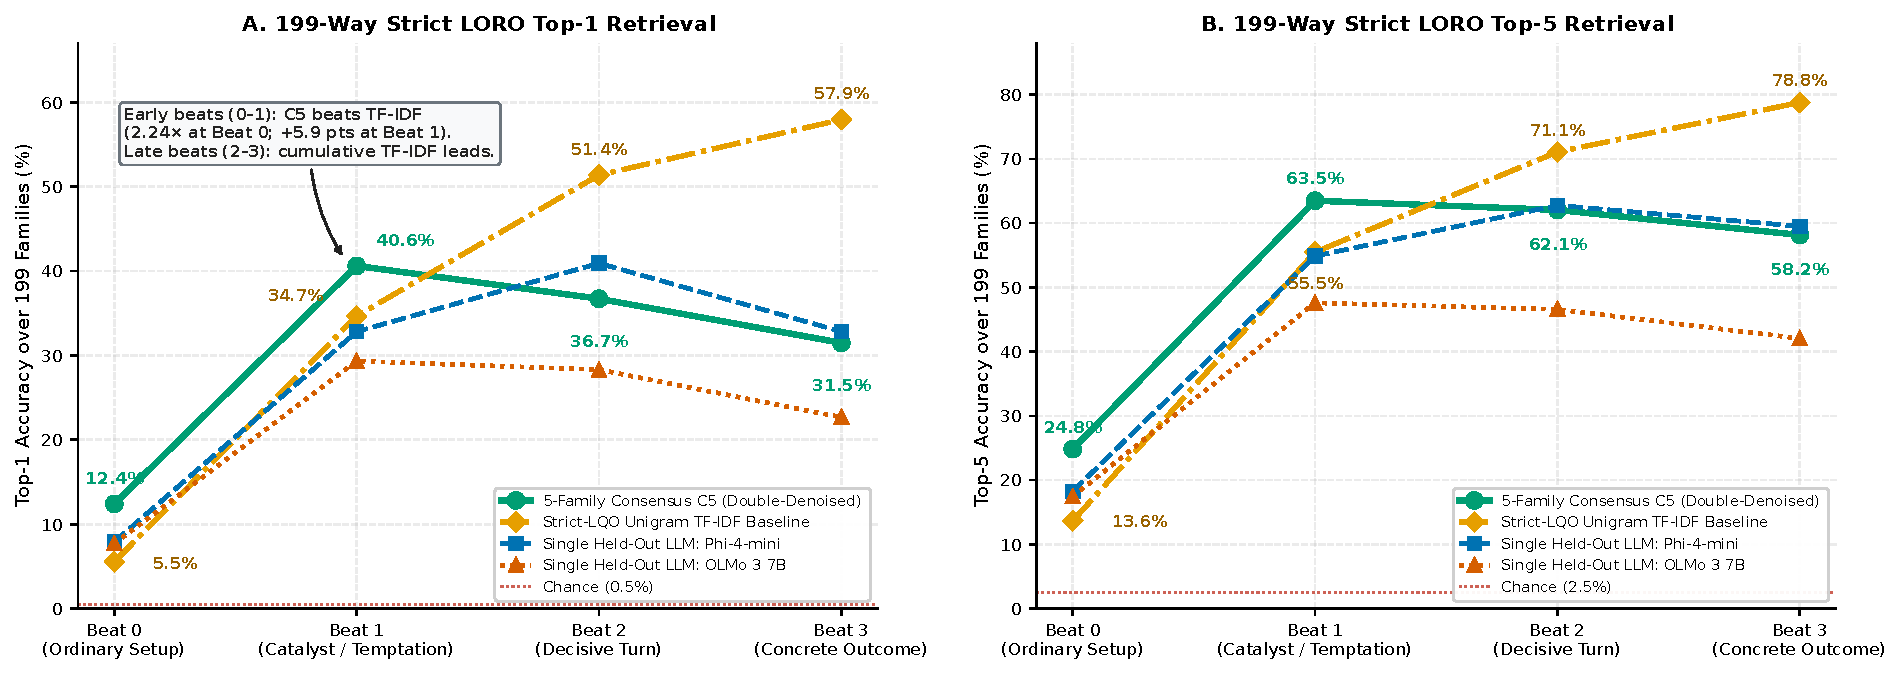
\includegraphics[width=\textwidth]{figures/fig3_loro_myth_amplification.pdf}
\caption{Strict leave-query-out 199-family retrieval across four cumulative narrative beats comparing frozen \texttt{C5}, 3.8B Phi-4-mini and 7B OLMo 3, and strict-LQO unigram TF-IDF.}
\label{fig:loro}
\end{figure*}

\subsubsection{24-Run 5M Cross-Tokenizer Distillation and 50\%-Depth Screen}
Table~\ref{tab:5m} and Fig.~\ref{fig:5m} summarize all 24 100M-token runs (3 seeds $\times$ 8 arms, 4.72M non-embed / 8.92M total, \texttt{bpe8k}). Supervising block 2 against \texttt{C5} raises held-out Phi-4 $R^2_{\text{frob}}$ from $-0.029$ (\texttt{P0}) and $+0.015$ (\texttt{P1}, Gemma 4 alone) to $+0.122$--$+0.132$, and OLMo 3 from $-0.073$ to $+0.130$--$+0.154$ with zero seed overlap (archived 5M logs used the earlier $R^2_{\text{opt}}$/retrieval scorer without affecting fixed-scale $R^2_{\text{frob}}$). Annealing $\texttt{plato\_w}\to0$ (\texttt{M0}) preserves held-out Phi-4 $R^2_{\text{frob}}$ ($+0.132$) after discarding the head. Upweighting 2D $U_{\text{jung}}$ (\texttt{M2} $3.5\times$ vs.\ \texttt{M3} $0.0\times$) lifts student-to-teacher \texttt{HOUSE} cosine (\texttt{bb\_cos}) from $+0.200$ to $+0.619$ ($3.1\times$) and zero-shot \texttt{SELF2} from $81.0\%$ to $94.9\%$ on the defining benchmark alongside a modest $3/3$ \texttt{BLiMP} edge ($0.657$ vs.\ $0.645$, $p\ge0.125$), while \texttt{mcq\_gain} falls on $3/3$ seeds ($+0.172\to+0.119$).

Distinct from the 24 100M-token runs, a 1-seed, 25M-token depth-placement screen (\texttt{v6\_distill50\_5m.json}) compared plain \texttt{D0\_ctrl} against 30\%-depth \texttt{L2} supervision (\texttt{D1}), 50\%-depth \texttt{L3} supervision (\texttt{D2}), and dual-depth \texttt{L2+L3} supervision (\texttt{D3}). At 50\% depth on the 2,395-passage neutral 6-model subset (accounting for tiny $\le 0.001$ offsets from Table~\ref{tab:gpa}'s 20,339-point corpus and Experiment 251's target package), teacher \texttt{C4} lifts Phi-4 $R^2_{\text{opt}}$ ($0.5948$ vs.\ $0.5457$ at 30\%) while OLMo 3 slips slightly ($0.5670\to0.5564$, with $R^2_{\text{frob}}$ $0.5099\to0.4960$) and Top-1 falls on both targets (Phi-4 $95.95\%\to91.78\%$, OLMo 3 $90.40\%\to88.74\%$). In the 5M student, \texttt{D2} selectively lifts \texttt{L3} 50\%-depth $R^2_{\text{opt}}$ (Phi-4 $0.2439\to0.3030$, OLMo 3 $0.2156\to0.2873$) and \texttt{D3} gains at both \texttt{L2} and \texttt{L3} ($0.3000$/$0.2982$ Phi-4 and $0.3028$/$0.2822$ OLMo 3). Those gains carry clear short-budget language modeling trade-offs (\texttt{books\_bpb} $1.6611\to1.6789$/$1.6759$, \texttt{chat\_bpb} $1.5401\to1.5876$/$1.5714$, \texttt{BLiMP} $0.6084\to0.6049$/$0.5918$, and procedural \texttt{mcq\_gain} $+0.0475\to+0.0150$/$+0.0050$), while 4.72M compositional swap probes stay near chance ($44.5\%$--$54.2\%$).

\begin{table*}[t]
\centering
\caption{Complete 3-seed means across all 24 5M (\texttt{bpe8k}, 4.72M non-embed / 8.92M total, 100M tokens) arms: plain control \texttt{P0}, constant $\texttt{plato\_w}=0.25$ (\texttt{P1}--\texttt{P3}), and annealed $\texttt{plato\_w}\to0$ (\texttt{M0}--\texttt{M3}). Legend: Books/Chat = held-out bits per byte (bpb); \texttt{mcq} = reading-comprehension gain; \texttt{bb\_cos}/\texttt{zsH}/\texttt{zsS2} = kept block-2 \texttt{HOUSE} cosine and zero-shot \texttt{HOUSE}/\texttt{SELF2} accuracy on the 312 contrasts defining $U_{\text{jung}}$.}
\label{tab:5m}
\scriptsize
\setlength{\tabcolsep}{2.6pt}
\begin{tabular}{@{}lccccccc@{}}
\toprule
\textbf{Arm (3-Seed Mean)} & \textbf{Phi-4 Cos / $R^2_{\text{frob}}$} & \textbf{OLMo 3 Cos / $R^2_{\text{frob}}$} & \textbf{Books / Chat} & \textbf{BLiMP} & \textbf{COPA} & \textbf{\texttt{mcq}} & \textbf{\texttt{bb\_cos} / \texttt{zsH} / \texttt{zsS2}} \\
\midrule
\texttt{P0} Plain Control ($\texttt{plato\_w}=0$) & 0.5873 / $-0.029$ & 0.5258 / $-0.073$ & \textbf{1.4714} / \textbf{1.2235} & 0.655 & 0.524 & +0.155 & -- \\
\texttt{P1} Gemma 4 Only & 0.5978 / $+0.015$ & 0.5598 / $+0.051$ & 1.4788 / 1.2316 & 0.648 & 0.519 & +0.147 & -- \\
\texttt{P2} 5-Fam \texttt{C5} & 0.6577 / $+0.122$ & 0.6079 / $+0.147$ & 1.4780 / 1.2310 & 0.640 & 0.519 & +0.151 & -- \\
\texttt{P3} \texttt{C5} + Folklore & 0.6600 / $+0.128$ & \textbf{0.6105} / \textbf{+0.154} & 1.4830 / 1.2367 & 0.654 & 0.531 & +0.152 & -- \\
\midrule
\texttt{M0} Annealed \texttt{C5} & 0.6628 / \textbf{+0.132} & 0.6074 / $+0.139$ & 1.4796 / 1.2325 & 0.649 & \textbf{0.532} & +0.155 & +0.290 / 73.8\% / 82.7\% \\
\texttt{M1} + LORO Proto & 0.6626 / $+0.127$ & 0.6058 / $+0.130$ & 1.4792 / 1.2303 & 0.650 & 0.525 & +0.141 & +0.264 / 72.7\% / 81.4\% \\
\texttt{M2} + $3.5\times U_{\text{jung}}$ & 0.6599 / \textbf{+0.132} & 0.6047 / $+0.135$ & 1.4801 / 1.2321 & \textbf{0.657} & 0.514 & +0.119 & \textbf{+0.619 / 81.1\% / 94.9\%} \\
\texttt{M3} $- 0.0\times U_{\text{jung}}$ & \textbf{0.6639} / $+0.131$ & 0.6070 / $+0.135$ & 1.4778 / 1.2297 & 0.645 & 0.520 & \textbf{+0.172} & +0.200 / 67.0\% / 81.0\% \\
\bottomrule
\end{tabular}
\end{table*}

\begin{figure*}[t]
\centering
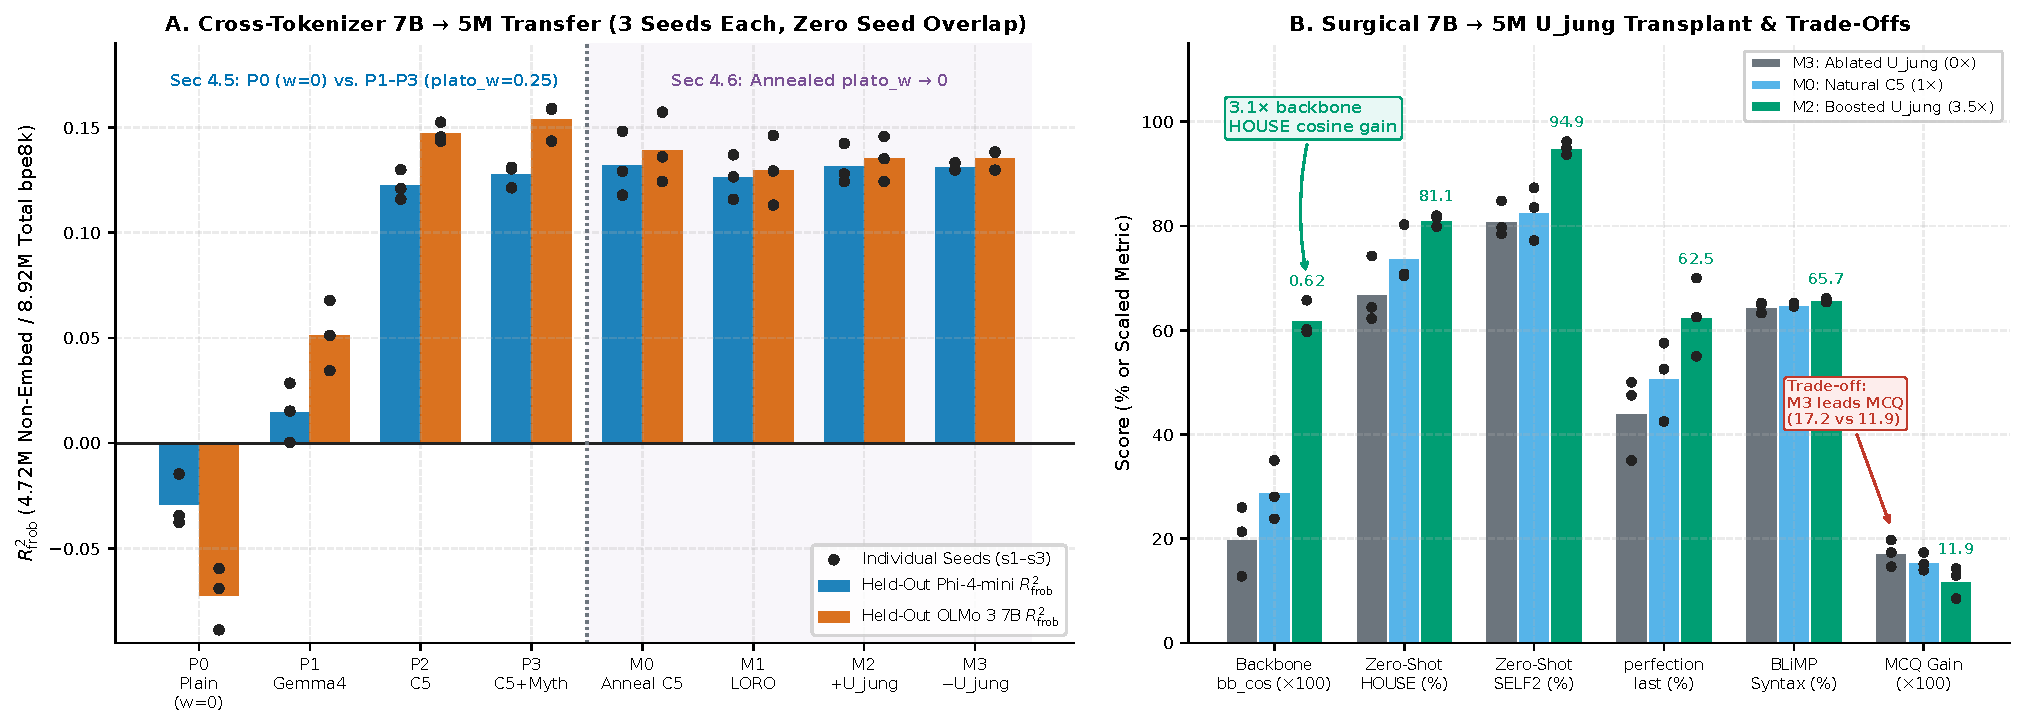
\includegraphics[width=\textwidth]{figures/fig4_5m_distillation_ujung.pdf}
\caption{\textbf{(A)} Held-out $R^2_{\text{frob}}$ across all eight 5M arms with per-seed dots confirming zero overlap over \texttt{P0} and \texttt{P1}. \textbf{(B)} Effect of $U_{\text{jung}}$ weighting (\texttt{M2} vs.\ \texttt{M0} vs.\ \texttt{M3}) on defining-benchmark alignment and the \texttt{mcq\_gain} trade-off.}
\label{fig:5m}
\end{figure*}

\subsection{Frontier 8B Causal Transplants, Epistemic Audit, and Dropped Claims}
\label{sec:8b}
\subsubsection{30\%-Depth Stage A Control (MLPs 11--12)}
Table~\ref{tab:8b} and Fig.~\ref{fig:8b} isolate the 30\%-depth \texttt{C5}+$U_{\text{jung}}$ objective on 8B multimodal \texttt{google/gemma-4-E4B-it} (seed 230; base $R^2_{\text{frob}}$ is $0.1825$/$0.2280$ in bf16 HuggingFace vs.\ $0.180$/$0.225$ in MLX Table~\ref{tab:gpa}). Stage A lifts held-out Phi-4 $R^2_{\text{frob}}$ by $+0.0245$ and OLMo 3 by $+0.0235$ over Base, outperforming the matched $\texttt{plato\_w}=0$ CE+KL control on all $8/8$ domain$\times$model cells (ratios of Base-referenced lifts $8.45\times$ Phi-4 and $7.12\times$ OLMo 3; 88.2\% and 86.0\% of total lift over Base comes beyond control). Gutenberg NLL sits $+0.0027$ above control ($4.8001$ vs.\ $4.7974$) with zero added inference parameters from the transplant and both multimodal verification fixtures passing.

\begin{table*}[t]
\centering
\caption{Matched $\texttt{plato\_w}=0.0$ CE+KL control at 30\% depth on 8B multimodal \texttt{google/gemma-4-E4B-it} (seed 230, 450 identical steps, MLPs 11--12, discarded head, zero extra inference parameters). Bottom row reports direct Stage A minus control difference, with parenthetical share of total lift over Base.}
\label{tab:8b}
\scriptsize
\setlength{\tabcolsep}{2.5pt}
\begin{tabular}{@{}lcccc>{\centering\arraybackslash}p{2.35cm}@{}}
\toprule
\textbf{8B Gemma 4 E4B Arm (30\%)} & \textbf{Phi-4 Cos / $R^2_{\text{frob}}$ (T1)} & \textbf{OLMo 3 Cos / $R^2_{\text{frob}}$ (T1)} & \textbf{\texttt{C5} Cos / $R^2_{\text{frob}}$} & \textbf{Gut NLL} & \textbf{Multimodal} \\
\midrule
Unmodified Base E4B & 0.6881 / +0.1825 (90.66\%) & 0.6557 / +0.2280 (85.81\%) & 0.8322 / +0.6119 & 5.0841 & Pass (``Red'' / ``blue pelican'') \\
Matched CE+KL Ctrl ($\texttt{plato\_w}=0$) & 0.6893 / +0.1854 (91.01\%) & 0.6568 / +0.2313 (86.08\%) & 0.8332 / +0.6146 & \textbf{4.7974} & Frozen towers \\
\textbf{Stage A (\texttt{C5}$+3.5\times U_{\text{jung}}$)} & \textbf{0.6995 / +0.2070 (91.67\%)} & \textbf{0.6652 / +0.2515 (86.38\%)} & \textbf{0.8415 / +0.6347} & 4.8001 & \textbf{Directly verified} \\
\midrule
Difference (Stage A $-$ Ctrl) & \textbf{+0.0102 / +0.0216 (88.2\%)} & \textbf{+0.0084 / +0.0202 (86.0\%)} & \textbf{+0.0083 / +0.0201} & +0.0027 & 0 extra params \\
\bottomrule
\end{tabular}
\end{table*}

\begin{figure*}[t]
\centering
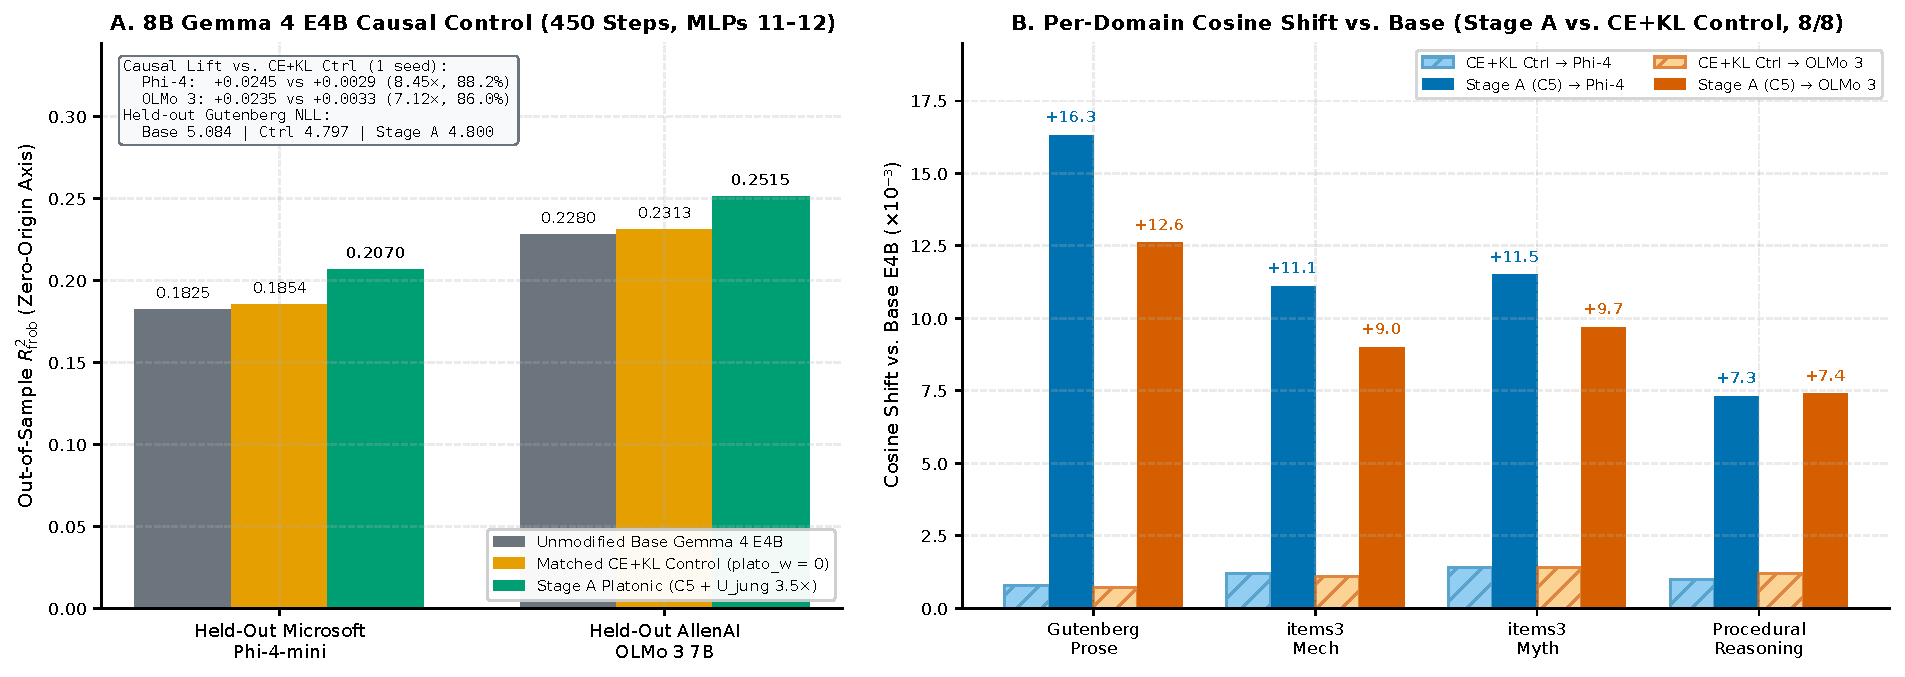
\includegraphics[width=\textwidth]{figures/fig5_8b_stage_a_causal.pdf}
\caption{Matched 3-arm control at 30\% depth on 8B \texttt{google/gemma-4-E4B-it}. \textbf{(A)} Matched CE+KL accounts for only 12--14\% of held-out-family $R^2_{\text{frob}}$ gains over Base. \textbf{(B)} Per-domain cosine lift across all $8/8$ domain$\times$model cells.}
\label{fig:8b}
\end{figure*}

\subsubsection{Experiment 251: Strictly Rival-Only 50\%-Depth Transplant (MLPs 19--20, 3 Seeds)}
\label{sec:exp251}
Stage A left two open questions: Gemma 4 contributed to \texttt{C5}, and mean-pool compositional readout strengthens from 30\% to 50\% depth (Section~\ref{sec:actor_depth}). Experiment 251 tests both across three paired training-order seeds (251, 252, 253) on official 8B \texttt{google/gemma-4-E4B-it} (\texttt{PLATO50\_LAYER} $=20$, MLPs 19--20, neutral \texttt{gut+proc+chat} passages, exact layer-12 invariance $\max|\Delta|=0.0$ across all 9 trained checkpoints on the 16-passage token-mean probe by construction; Table~\ref{tab:exp251}, Fig.~\ref{fig:exp251}). Pre-training diagnostics inspected on the two excluded target families (\texttt{e4b\_transplant50\_teacher\_diag.json}, MLX precision; Base Phi-4 $R^2_{\text{frob}}=0.0623$ vs.\ bf16 HF $0.0619$) show that between tested single teachers (Gemma 4 and Qwen3.5), Base Gemma 4 aligns worst at 50\% depth (Phi-4 $+0.0623$, OLMo 3 $+0.0594$). Removing Gemma 4 therefore yields a cleaner teacher on $R^2_{\text{frob}}$: rival-only \texttt{C3\_50} (Qwen3.5 + Llama 3.1 + Mistral) beats 4-family \texttt{C4\_50} on Phi-4 ($R^2_{\text{frob}}=0.5733$ vs.\ $0.5450$, Top-1 $92.59\%$ vs.\ $91.78\%$) and on OLMo 3 $R^2_{\text{frob}}$ ($0.5104$ vs.\ $0.4963$, with OLMo 3 Top-1 tied at $88.66\%$ vs.\ $88.74\%$). Because these target diagnostics were inspected before training, teacher selection is not independent of the two target families; the valid held-out units are the scoring folds, and both target families remain excluded from teacher construction.

Training on \texttt{C3\_50} reproduces the alignment gain across all three paired seeds (Table~\ref{tab:exp251}, sample SD with $ddof=1$, computed from full-precision per-seed metrics). Moving MLPs 19--20 by $0.99\%$ (L19) and $1.06\%$ (L20) relative L2 norm lifts held-out-family Phi-4 $R^2_{\text{frob}}$ to $+0.1583\pm0.0010$ ($+0.0963\pm0.0010$ over Base $+0.0619$, closing 18.8\% of the gap to teacher \texttt{C3\_50}, with Top-1 $+6.96\pm0.27$ pp over Base / $+6.30\pm0.16$ pp over \texttt{ctrl50}) and by \textbf{$+0.0869\pm0.0017$} over matched \texttt{ctrl50} ($+0.0714\pm0.0012$, per-seed deltas $+0.0888, +0.0864, +0.0855$, 3/3 seeds, 3-seed $t$-interval $\pm0.0042$). On OLMo 3, \texttt{c3\_50} reaches $+0.1466\pm0.0009$ ($+0.0878\pm0.0009$ over Base $+0.0588$, closing 19.4\% of the teacher gap, with Top-1 $+3.97\pm0.10$ pp over Base / $+4.14\pm0.12$ pp over \texttt{ctrl50}) and beats \texttt{ctrl50} ($+0.0686\pm0.0013$) by \textbf{$+0.0780\pm0.0017$} (per-seed $+0.0799, +0.0777, +0.0765$, 3/3 seeds, 3-seed $t$-interval $\pm0.0042$). Because \texttt{ctrl50}'s Base-referenced lift is small ($+0.0094\pm0.0012$ Phi-4, $+0.0098\pm0.0013$ OLMo 3), Base-referenced lift ratios vary across seeds ($8.9\times$--$11.5\times$, ratio of 3-seed mean lifts $10.2\times$ Phi-4; $7.8\times$--$10.1\times$, ratio of mean lifts $9.0\times$ OLMo 3), whereas direct \texttt{c3\_50}$-$\texttt{ctrl50} margins have tight seed dispersion. Resampling the 400 evaluation passage groups conditional on the three fitted seeds using the exact canonical domain-stratified 2-fold Procrustes predictions (\texttt{Random(2288)}, train-fold centering and affine map) gives clause-weighted cosine deltas over \texttt{ctrl50} of $+0.03632$ (pct $[+0.03533, +0.03733]$, basic $[+0.03531, +0.03731]$) on Phi-4 and $+0.03163$ (pct $[+0.03067, +0.03263]$, basic $[+0.03063, +0.03259]$) on OLMo 3, matching the headline point-weighted deltas ($+0.0363\pm0.0006$ and $+0.0316\pm0.0004$); equal-group-weighted passage means on the same canonical predictions are $+0.03841$ ($[+0.03685, +0.04004]$) and $+0.03408$ ($[+0.03276, +0.03544]$). Across all 24/24 dependent seed$\times$domain$\times$model cells (for example, held-out \texttt{held\_gut} cosine $+0.0614\pm0.0006$ Phi-4 and $+0.0542\pm0.0013$ OLMo 3 over Base, $+0.0577$/$+0.0508$ over \texttt{ctrl50}), rival-only \texttt{c3\_50} beats both \texttt{ctrl50} and Gemma-including \texttt{c4\_50} ($+0.0247\pm0.0014$ Phi-4 and $+0.0207\pm0.0014$ OLMo 3 $R^2_{\text{frob}}$, 3/3 seeds).

The mechanistic boundary is equally clear across seeds. Both \texttt{ctrl50} and \texttt{c3\_50} improve held-out Gutenberg NLL over Base ($5.0841\to4.5301\pm0.0042$ and $4.5340\pm0.0038$), with \texttt{c3\_50} incurring a small consistent NLL penalty of $+0.0039\pm0.0024$ over \texttt{ctrl50} (per-seed $+0.0047, +0.0012, +0.0057$; 40-passage bootstrap conditional on the three seeds pct $[+0.00071, +0.00713]$, basic $[+0.00062, +0.00704]$). Procedural MCQ shows a zero observed mean difference ($84.33\%$ vs.\ $84.33\%$, per-seed $+0.50, 0.00, -0.50$ pp, mean $0.00\pm0.50$ pp, 400-item bootstrap $[-0.92, +0.92]$ pp), \texttt{bm\_actor2x2} NLL stays intact ($66.94\%$/$73.19\%$), and all 10/10 checkpoints (Base plus 9 trained) pass both color (``Red'') and speech (``blue pelican'') fixtures. On label-free-trained weights evaluated with supervised (\texttt{cv2}) and zero-shot (\texttt{zs}) probes, downstream probing shows mixed probe-specific shifts with no overall gain over \texttt{ctrl50}: \texttt{bm\_actor2x2} within-native \texttt{cv2} mean dips on 3/3 seeds ($80.92\%$ vs.\ $81.15\%$, $-0.22\pm0.01$ pp), cross-family \texttt{g2r\_cv2} on the two held-out families is $68.97\%$ vs.\ $68.81\%$ ($+0.16\pm0.74$ pp, range $[-0.68, +0.71]$), zero-shot \texttt{g2r\_zs} is $60.90\%$ vs.\ $61.25\%$ ($-0.35\pm0.12$ pp), and \texttt{HOUSE}$\to$\texttt{SELF2} reaches $100.0\%$ on 3/3 seeds (vs.\ $98.73\%$ Base/\texttt{ctrl50}). Against unmodified Base, rival$\to$Gemma supervised transfer dips slightly (\texttt{r2g\_cv2\_all5} $-0.58\pm0.20$ pp and \texttt{r2g\_cv2\_teacher3} $-0.73\pm0.31$ pp). Neutral alignment reliably shifts mid-layer geometry toward cross-family consensus without automatically improving downstream reasoning or probing accuracy.

\begin{table*}[t]
\centering
\caption{Experiment 251: 3-seed (seeds 251, 252, 253) paired 50\%-depth transplant on 8B multimodal \texttt{google/gemma-4-E4B-it} (450 neutral steps, MLPs 19--20, exact L12 invariance $\max|\Delta|=0.0$ across 9 trained checkpoints on the 16-passage probe by construction, and color/speech pass on 10/10 checkpoints; \texttt{e4b\_transplant50\_exp251.json}). Legend: Cos = 3-seed mean point-weighted cosine; $R^2_{\text{frob}}$ = 3-seed mean $\pm$ SD ($ddof=1$); ($R^2_{\text{opt}}$, T1) = 3-seed mean strict $R^2$ and Top-1 (unrounded full precision); Act.\ Nat.\ = 3-seed mean within-native \texttt{cv2} on \texttt{bm\_actor2x2\_247}. Ratios of 3-seed mean Base-referenced $R^2_{\text{frob}}$ lifts (\texttt{c3\_50} vs.\ \texttt{ctrl50}) are $10.2\times$ ($+0.0963$ vs.\ $+0.0094$, per-seed $8.9\times$--$11.5\times$) on Phi-4 and $9.0\times$ ($+0.0878$ vs.\ $+0.0098$, per-seed $7.8\times$--$10.1\times$) on OLMo 3.}
\label{tab:exp251}
\scriptsize
\setlength{\tabcolsep}{1.1pt}
\begin{tabular}{@{}lcccccc@{}}
\toprule
\textbf{Arm (50\%, 3 Seeds)} & \textbf{Phi-4 Cos/$R^2_{\text{frob}}\pm$SD ($R^2_{\text{opt}}$, T1)} & \textbf{OLMo 3 Cos/$R^2_{\text{frob}}\pm$SD ($R^2_{\text{opt}}$, T1)} & \textbf{Gut NLL} & \textbf{MCQ (Gain)} & \textbf{Act.\ Nat.} & \textbf{L12/V\&A} \\
\midrule
Base E4B & 0.6154 / +0.0619 (0.269, 68.4\%) & 0.5874 / +0.0588 (0.267, 71.6\%) & 5.0841 & 79.8\% (+58.0) & 81.56\% & 0.0/Pass \\
\texttt{ctrl50} ($w=0$) & 0.6189 / +0.0714$\pm$0.0012 (0.275, 69.0\%) & 0.5908 / +0.0686$\pm$0.0013 (0.272, 71.5\%) & \textbf{4.5301} & 84.3\% (+63.3) & 81.15\% & 0.0/3/3 \\
\texttt{c4\_50} (+G4) & 0.6449 / +0.1336$\pm$0.0012 (0.310, 74.3\%) & 0.6141 / +0.1259$\pm$0.0012 (0.305, 75.1\%) & 4.5333 & 84.3\% (+63.2) & 80.94\% & 0.0/3/3 \\
\textbf{\texttt{c3\_50} (0 G4)} & \textbf{0.6553 / +0.1583$\pm$0.0010 (0.325, 75.3\%)} & \textbf{0.6224 / +0.1466$\pm$0.0009 (0.318, 75.6\%)} & 4.5340 & 84.3\% (+62.9) & 80.92\% & \textbf{0.0/3/3} \\
\midrule
\texttt{c3\_50}$-$\texttt{ctrl50} & \textbf{+0.0363 / +0.0869$\pm$0.0017 (+6.3 pp)} & \textbf{+0.0316 / +0.0780$\pm$0.0017 (+4.1 pp)} & +0.0039 & 0.0 pp (n.s.) & $-0.22$ & 0 extra \\
\bottomrule
\end{tabular}
\end{table*}

\begin{figure*}[t]
\centering
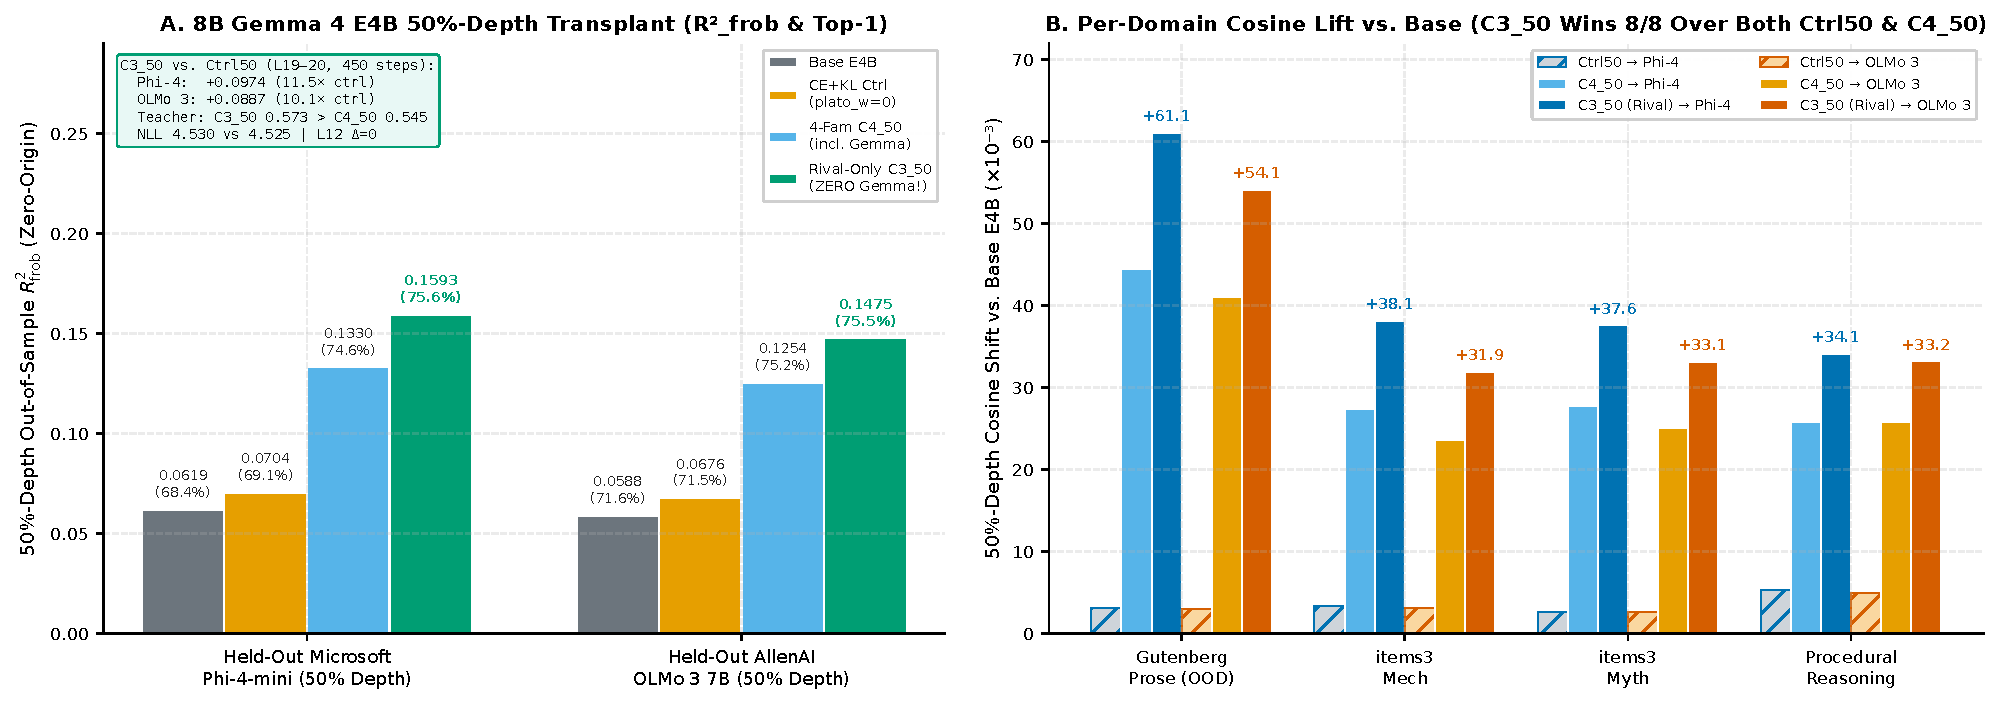
\includegraphics[width=\textwidth]{figures/fig8_e4b_50pct_transplant.pdf}
\caption{Experiment 251: 3-seed paired 50\%-depth transplant on 8B \texttt{google/gemma-4-E4B-it} (seeds 251--253, MLPs 19--20, exact L12 invariance $\max|\Delta|=0.0$). \textbf{(A)} 3-seed mean $R^2_{\text{frob}}$ with individual seed dots: rival-only \texttt{C3\_50} (zero Gemma 4) beats both \texttt{ctrl50} and \texttt{C4\_50} on 3/3 seeds. \textbf{(B)} Per-domain 3-seed mean cosine shift vs.\ Base ($\pm$SD): \texttt{C3\_50} wins all 24/24 dependent seed$\times$domain$\times$model cells.}
\label{fig:exp251}
\end{figure*}

\subsubsection{Native-Layer Epistemic Probing and Three Dropped Follow-Up Audits}
\label{sec:epi}
In each model's native 40\%/60\% residual stream, raw \texttt{CORRECTNESS} (20 true/false pairs \cite{marks2024geometry}) and \texttt{HOUSE} show depth-dependent cosines ($+0.2230$ at L17, $+0.0887$ at L25 on Base Gemma 4; $+0.1571$ at L12, $-0.0033$ at L19 on Base Qwen3.5). Gram-Schmidt orthogonalization $u_{\text{house},\perp} = \text{unit}(u_{\text{house}} - (u_{\text{house}}\cdot u_{\text{corr}}) u_{\text{corr}})$ removes input overlap ($\cos=0.000$) with frozen calibration scaling.

On 24 zero-entity-overlap minimal pairs (12 false presuppositions + 12 public-known vs.\ inaccessible private facts) across 12 matched cells plus \texttt{Dedup-10} (Table~\ref{tab:epi}, Fig.~\ref{fig:epi}), adding the Aion system prompt shifts the two unknown subsets in opposite first-token entropy directions. Pooled symmetric first-token entropy AUROC falls from $0.913$/$0.951$ (Neutral) to $0.521$ (Base Gemma 4), $0.576$ (Stage B), and $0.596$ (Base Qwen3.5). Averaged \texttt{Combined\_Perp} clears nominal per-cell $p<0.05$ against 500 mirrored random pairs in $11/12$ cells ($6/12$ Holm, $10/12$ Benjamini--Hochberg false discovery rate [BH-FDR]; solo \texttt{-HOUSE\_PERP} $5/12$ nominal, $0/12$ Holm/BH), failing at Qwen3.5 L19 Neutral ($0.573$, $p=0.409$ n.s.) and reaching $1.000$ on \texttt{Dedup-10}. Direct sentiment control (\texttt{valence\_ctrl234.json}) splits cleanly by prompt: under Aion prompting, pure \texttt{-SENTIMENT\_PERP} matches or exceeds \texttt{-HOUSE\_PERP} in all four Base cells (removing $u_{\text{sent}}$ drops Qwen L19 Aion \texttt{-HOUSE\_PERP\_BOTH} to $0.519$, $p=0.475$ n.s.). Under Neutral prompting at Gemma L25, \texttt{-SENTIMENT\_PERP} fails ($0.602$, $p=0.375$ n.s.) while \texttt{-HOUSE\_PERP\_BOTH} hits $1.000$ ($p=0.002$, $+0.033\,[+0.003,+0.076]$ over \texttt{-CORR}).

\paragraph*{Explicitly Dropped Follow-Up Audits (Exps 241, 243, 244)}
Three follow-up audits (\texttt{v6\_dropped\_and\_depth\_audits.json}) failed our internally specified decision criteria and are explicitly dropped, with three distinct failure modes:
\begin{enumerate}
  \item \textbf{Exp 244 (120-pair matched-pair epistemic generalization; inadmissible benchmark):} Scaling the epistemic audit to 120 entity- and word-count-matched pairs (\texttt{epi\_matched245\_data.json}; capitalization AUROC $0.500$, word-count AUROC $0.501$) across four 50\%-depth models (Gemma 4, Qwen3.5, Llama 3.1, OLMo 3) failed our internally specified admissibility gate on 4/4 models: random single-direction 95th-percentile AUROC reached $0.759$--$0.980$ (exceeding the $\le 0.70$ ceiling), and \texttt{Combined\_Perp} cleared $0/4$ Holm tests against \texttt{CORR} plus 500 random directions ($p_{\text{holm}}=0.064$--$0.463$). Table~\ref{tab:epi} therefore stays bounded to its 24-pair benchmark.
  \item \textbf{Exp 241 (Single-layer cross-family causal steering/ablation; null causal effect):} Steering rotated binding directions at a single 50\% layer ($\alpha=1.0$) across three pairs (\texttt{bm120} / \texttt{bm\_rel242}) gave weak logit shifts ($+0.0258$/$+0.0227$ Gemma$\to$Qwen, $+0.0415$/$+0.0384$ Gemma$\to$Llama, $-0.0070$/$+0.0052$ Qwen$\to$OLMo) and near-zero flip rates ($0.0\%$--$2.5\%$), while centered ablation gave a null functional interaction (\texttt{bm\_rel242} $-0.0070\,[-0.0156,+0.0019]$). Section~\ref{sec:actor_depth} is therefore limited to a linear readout rather than causal localization.
  \item \textbf{Exp 243 (14-text systems-archetype replication; underperforming representation):} On 14 external public systems-archetype passages \cite{nordfors2026archetypal,senge1990fifth}, 50\%-depth \texttt{C4} pattern-over-topic AUROC trailed unigram BoW on both matched cohorts: $0.493$ vs.\ $0.625$ (cross-topic pattern $0.823$) on the 12 English texts, and $0.602$ vs.\ $0.658$ (cross-topic $0.809$) on all 14 texts. Although underpowered at $n=14$, this is our sole test on third-party stimuli and directly qualifies Section~\ref{sec:distill}'s early-arc retrieval finding.
\end{enumerate}

\begin{table*}[t]
\centering
\caption{Cross-model native-layer epistemic audit across 12 matched 40\%/60\%-depth cells (24 minimal pairs) plus Dedup-10. Input vectors satisfy $\cos(u_{\text{corr}}, u_{\text{house},\perp})=0.000$; empirical $p=(k+1)/501$. Legend: 1st-Tok Ent = mean known$\to$unknown first-token entropy (nats); Sym.\ Ent = best-sign symmetric entropy AUROC; \texttt{H\_PERP} = \texttt{HOUSE} orthogonal to \texttt{CORR}; \texttt{Comb\_Perp} = averaged score (paired accuracy, $p$); Null 95 = 95th-percentile AUROC of 500 random mirrored pairs. Follow-up 120-pair scaling (Exp 244) failed admissibility and is dropped.}
\label{tab:epi}
\scriptsize
\setlength{\tabcolsep}{2.4pt}
\begin{tabular}{@{}lcccccc@{}}
\toprule
\textbf{Model, Prompt \& Layer} & \textbf{1st-Tok Ent} & \textbf{Sym.\ Ent} & \textbf{$-$\texttt{CORR} ($p$)} & \textbf{$-$\texttt{H\_PERP} ($p$)} & \textbf{\texttt{Comb\_Perp} (Pair, $p$)} & \textbf{Null 95} \\
\midrule
Gemma 4 Base $\times$ Neutral (L17, 40\%) & $0.063\to0.443$ & 0.913 & 0.995 (0.002) & 0.819 (0.122 n.s.) & \textbf{0.988} (100\%, \textbf{0.004}) & 0.896 \\
Gemma 4 Base $\times$ Aion (L17, 40\%) & $1.307\to1.270$ & \textbf{0.521} & 0.870 (0.056 n.s.) & 0.856 (0.076 n.s.) & \textbf{0.875} (91.7\%, \textbf{0.048}) & 0.868 \\
Gemma 4 Stage-B (ON) $\times$ Neutral (L17) & $0.194\to0.507$ & 0.743 & 0.995 (0.002) & 0.552 (0.461 n.s.) & \textbf{0.990} (100\%, \textbf{0.004}) & 0.898 \\
Gemma 4 Stage-B (ON) $\times$ Aion (L17) & $0.736\to0.750$ & \textbf{0.576} & 0.904 (0.016) & 0.639 (0.303 n.s.) & \textbf{0.911} (95.8\%, \textbf{0.022}) & 0.863 \\
\midrule
Gemma 4 Base $\times$ Neutral (L25, 60\%) & $0.063\to0.443$ & 0.913 & 0.957 (0.036) & 0.981 (0.020) & \textbf{0.988} (95.8\%, \textbf{0.010}) & 0.932 \\
Gemma 4 Base $\times$ Aion (L25, 60\%) & $1.307\to1.270$ & \textbf{0.521} & 0.957 (0.058 n.s.) & 0.962 (0.054 n.s.) & \textbf{0.998} (100\%, \textbf{0.002}) & 0.941 \\
Gemma 4 Stage-B (ON) $\times$ Neutral (L25) & $0.194\to0.507$ & 0.743 & 0.993 (0.014) & 0.984 (0.020) & \textbf{1.000} (100\%, \textbf{0.004}) & 0.936 \\
Gemma 4 Stage-B (ON) $\times$ Aion (L25) & $0.736\to0.750$ & \textbf{0.576} & 0.984 (0.012) & 0.977 (0.020) & \textbf{0.998} (100\%, \textbf{0.006}) & 0.938 \\
\midrule
Qwen3.5-9B Base $\times$ Neutral (L12, 40\%) & $0.190\to1.083$ & 0.951 & 0.903 (0.004) & 0.844 (0.030) & \textbf{0.943} (87.5\%, \textbf{0.002}) & 0.809 \\
Qwen3.5-9B Base $\times$ Aion (L12, 40\%) & $1.290\to1.101$ & \textbf{0.596} & 0.861 (0.026) & 0.762 (0.120 n.s.) & \textbf{0.865} (87.5\%, \textbf{0.030}) & 0.830 \\
Qwen3.5-9B Base $\times$ Neutral (L19, 60\%) & $0.190\to1.083$ & 0.951 & 0.571 (0.387 n.s.) & 0.571 (0.387 n.s.) & 0.573 (62.5\%, 0.409 n.s.) & 0.904 \\
Qwen3.5-9B Base $\times$ Aion (L19, 60\%) & $1.290\to1.101$ & \textbf{0.596} & 0.873 (0.090 n.s.) & \textbf{0.974} (\textbf{0.006}) & \textbf{0.948} (87.5\%, \textbf{0.024}) & 0.913 \\
\midrule
\textit{Dedup-10 Nonce:} Gemma 4 Base (L25) & $1.235\to1.414$ & \textbf{0.570} & 0.950 (0.082 n.s.) & 0.990 (0.044) & \textbf{1.000} (100\%, \textbf{0.038}) & 0.980 \\
\textit{Dedup-10 Nonce:} Gemma 4 Stage-B (L25) & $0.642\to1.046$ & \textbf{0.540} & 0.980 (0.028) & \textbf{1.000} (\textbf{0.014}) & \textbf{1.000} (100\%, \textbf{0.016}) & 0.951 \\
\bottomrule
\end{tabular}
\end{table*}

\begin{figure*}[t]
\centering
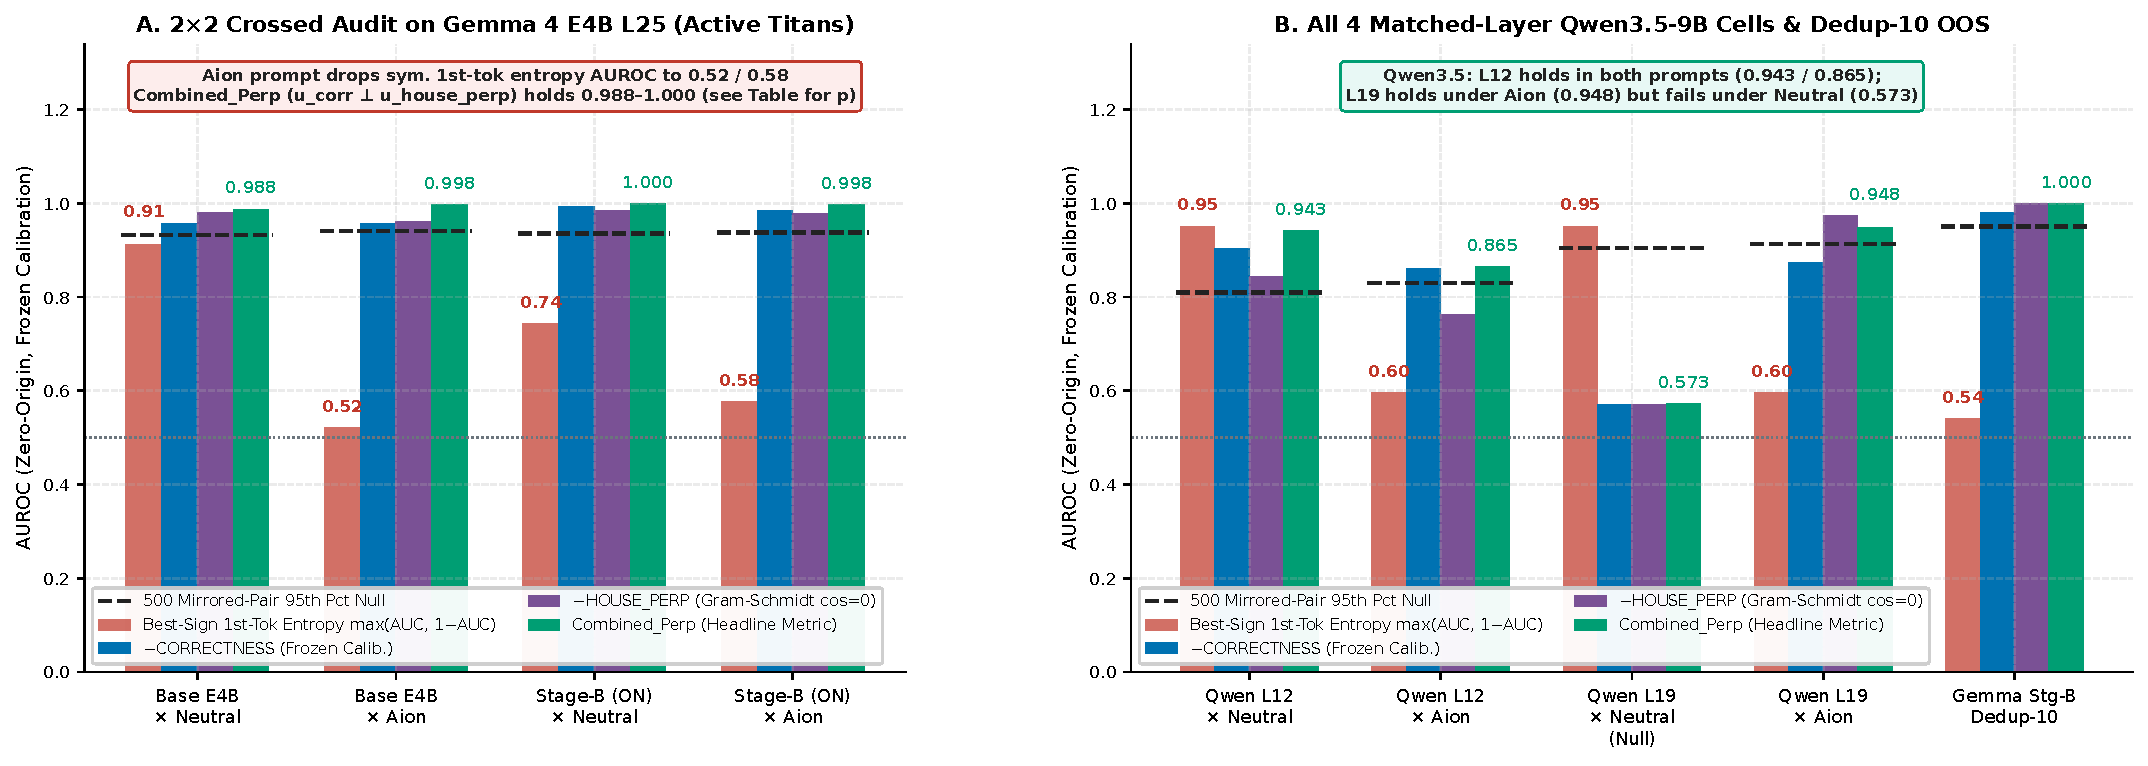
\includegraphics[width=\textwidth]{figures/fig6_epistemic_house_correctness.pdf}
\caption{Zero-origin AUROC for native-layer epistemic probing. \textbf{(A)} Gemma 4 E4B L25: Aion prompting drops symmetric first-token entropy AUROC to 0.52/0.58 while \texttt{Combined\_Perp} holds 0.988--1.000. \textbf{(B)} All four matched-layer Qwen3.5-9B cells (including the explicit L19 Neutral null) and Dedup-10.}
\label{fig:epi}
\end{figure*}

\section{Discussion, Practical Uses, and Limitations}
\label{sec:discussion}
\subsection{Statistical Projection vs.\ Psyche: Culture, Development, and Consciousness}
\label{sec:psyche}
Why do independently trained LLMs share a transferable mid-depth relational geometry and absorb a rival-only 50\%-depth consensus (\texttt{C3\_50}) over matched control, yet show no advantage for study-selected Jung-inspired labels over unlabeled corpus PCA or everyday family roles (even though Jungian labels outscore workplace labels on ATU $v_{\text{dir}}$, $0.13803$ vs.\ $0.07300$, Holm-7 $p=0.007$)? Analytical psychology makes a helpful conceptual distinction here. Jung insisted that ``the archetypal representations (images and ideas) mediated to us by the unconscious should not be confused with the archetype as such'' \cite{jung1969structure} (CW 8, \P417). For Jung, the \textit{archetype-as-such} is an irrepresentable formal predisposition (``The representations themselves are not inherited, only the forms'' \cite{jung1968archetypes}, CW 9.I, \P155), placed ``beyond the psychic sphere, analogous to the position of physiological instinct, which is immediately rooted in the stuff of the organism'' \cite{jung1969structure} (CW 8, \P420).

Our empirical design measures neither biological inheritance nor subjective experience. We neither assert nor deny machine psyche; instead, we treat aligned subspaces as a statistical projection of human-authored training data flattened into model weights (Fig.~\ref{fig:projection}). Within analytical psychology and comparative folklore, cultural-transmission accounts \cite{roesler2012archetypes,dasilva2016comparative,thuillard2018large,huggins2021jung}, evolved cognitive-attractor accounts \cite{goodwyn2010approaching,goodwyn2013recurrent}, and developmental emergentist models \cite{hogenson2001baldwin,knox2003archetype} offer competing mechanisms for why human stories recur. Because LLMs learn from human cultural records (filtered further by collector choices, translation, and ordinary semantic similarity), our text-only experiments cannot empirically settle debates among biological inheritance, cultural diffusion, and developmental emergence. As an interpretive synthesis separate from what the data decide (a reading Roesler does not himself endorse, since he argues against biological innateness \cite{roesler2012archetypes}), we view Goodwyn's evolved cognitive attractors \cite{goodwyn2010approaching,goodwyn2013recurrent} and Roesler's cultural-transmission account \cite{roesler2012archetypes} as addressing different levels of Jung's crystal-lattice distinction \cite{jung1968archetypes} (CW 9.I, \P155): a hereditary biological substrate and evolved cognitive attractors (alongside Hogenson's Baldwinian emergence and Knox's developmental \textit{image schemas} \cite{hogenson2001baldwin,knox2003archetype}) shape the empty formal predispositions (the axial lattice), while cultural dissemination of myths, religion, and literature supplies the materialized archetypal images that fill it. Empirically, our measurements establish only the narrower point that recurring narrative and relational patterns in human corpora are regular enough to align across seven labs and transfer across tokenizers.

\begin{figure}[t]
\centering
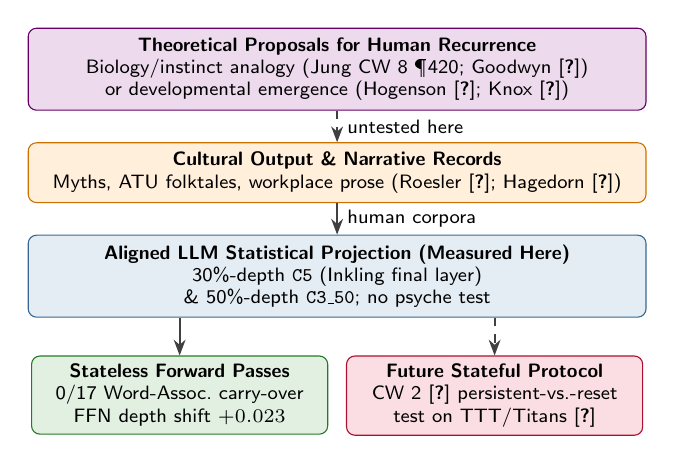
\begin{tikzpicture}[
    node distance=0.40cm and 0.20cm,
    nbox/.style={rectangle, rounded corners=3pt, draw=#1!80!black, fill=#1!14, text=black,
      text width=7.6cm, minimum height=0.68cm, align=center, font=\sffamily\scriptsize, inner sep=3.5pt},
    sbox/.style={rectangle, rounded corners=3pt, draw=#1!80!black, fill=#1!14, text=black,
      text width=3.55cm, minimum height=0.84cm, align=center, font=\sffamily\scriptsize, inner sep=3pt},
    arr/.style={-{Stealth[length=2mm]}, thick, draw=black!75}
]
  \node[nbox=accentpurple] (arch) {\textbf{Theoretical Proposals for Human Recurrence}\\Biology/instinct analogy (Jung CW 8 \P420; Goodwyn \cite{goodwyn2013recurrent})\\or developmental emergence (Hogenson \cite{hogenson2001baldwin}; Knox \cite{knox2003archetype})};
  \node[nbox=accentorange, below=of arch] (cult) {\textbf{Cultural Output \& Narrative Records}\\Myths, ATU folktales, workplace prose (Roesler \cite{roesler2012archetypes}; Hagedorn \cite{hagedorn2022bearing})};
  \node[nbox=accentblue, below=of cult] (proj) {\textbf{Aligned LLM Statistical Projection (Measured Here)}\\30\%-depth \texttt{C5} (Inkling final layer) \& 50\%-depth \texttt{C3\_50}; no psyche test};
  \node[sbox=accentgreen, below=0.48cm of proj, xshift=-2.0cm] (stat) {\textbf{Stateless Forward Passes}\\0/17 Word-Assoc.\ carry-over\\FFN depth shift $+0.023$};
  \node[sbox=accentred, below=0.48cm of proj, xshift=2.0cm] (dyn) {\textbf{Future Stateful Protocol}\\CW 2 \cite{jung1973experimental} persistent-vs.-reset\\test on TTT/Titans \cite{behrouz2024titans}};

  \draw[arr, dashed] (arch) -- node[right, font=\sffamily\scriptsize] {untested here} (cult);
  \draw[arr] (cult) -- node[right, font=\sffamily\scriptsize] {human corpora} (proj);
  \draw[arr] (proj.south -| stat.north) -- (stat.north);
  \draw[arr, dashed] (proj.south -| dyn.north) -- (dyn.north);
\end{tikzpicture}
\caption{Methodological scope separating theoretical accounts of human archetypal recurrence \cite{jung1969structure,goodwyn2013recurrent,hogenson2001baldwin,knox2003archetype}, cultural records \cite{roesler2012archetypes,hagedorn2022bearing}, the aligned LLM projections measured here (\texttt{C5} at $\sim$30\% depth and \texttt{C3\_50} at 50\% depth), and a falsifiable stateful Word Association Test (WAT) protocol for future test-time training (TTT) systems \cite{jung1973experimental,behrouz2024titans}.}
\label{fig:projection}
\end{figure}

This boundary also clarifies active debates over AI consciousness. Public statements from AI researchers span open uncertainty and speculative claims: Anthropic CEO Dario Amodei said in February 2026 that ``We don't know if the models are conscious. We are not even sure that we know what it would mean for a model to be conscious or whether a model can be conscious. But we're open to the idea that it could be'' \cite{amodei2026conscious}, whereas Ilya Sutskever conjectured in 2022 that ``it may be that today's large neural networks are slightly conscious'' \cite{sutskever2022slightly}. Philosophers and cognitive scientists have focused on empirical indicators: David Chalmers argued in April 2023 that ``while it is somewhat unlikely that current large language models are conscious, we should take seriously the possibility that successors to large language models may be conscious in the not-too-distant future'' \cite{chalmers2023could}, and Butlin, Long, Elmoznino, Bengio, Birch, and colleagues concluded in 2023 that ``Our analysis suggests that no current AI systems are conscious, but also suggests that there are no obvious technical barriers to building AI systems which satisfy these indicators'' \cite{butlin2023consciousness}. Murray Shanahan and colleagues further warn against anthropomorphic language and against mistaking role-play by next-token predictors for inner mental life \cite{shanahan2024talking,shanahan2023roleplay}.

As a speculative theoretical note, distinct from our empirical results, Jung defines the psyche as ``the totality of all psychic processes, conscious as well as unconscious'' \cite{jung1971types} (CW 6, \P797) and defines consciousness as ``the relation of psychic contents to the ego, in so far as this relation is perceived as such by the ego'' \cite{jung1971types} (CW 6, \P700). Elsewhere, Jung writes that the ego ``rests on two seemingly different bases: the somatic and the psychic'' \cite{jung1968aion} (CW 9.II, \P3), and compares inherited archetypal forms to biological instincts \cite{jung1968archetypes} (CW 9.I, \P155). Late Jung's \textit{psychoid} concept \cite{jung1969structure} (CW 8, \P420) pulls beyond purely biological mechanisms into non-physiological territory, placing physiological instinct at one pole and archetype at an opposite pole that remains empirically unverifiable within computational text studies. On an organismic reading of Jung combined with the further philosophical premise that living biological organization is necessary for a psyche and for phenomenal experience, non-living language models lack both the conscious and unconscious components of a living, embodied psyche; they hold at best a statistical echo of human psychic structure, formed from the linguistic residue of relational patterns that human authors impart to language and literature. Under substrate-independent functionalist accounts \cite{chalmers2023could,butlin2023consciousness}, by contrast, lacking biological life does not settle whether an artificial system can be conscious. Our experiments do not test either philosophical premise. Empirically, our measurements are consistent with cross-family linear alignment arising from shared statistical structure in training corpora (alongside possible shared world structure or architectural biases that our probes do not separate).

Jung's 1904--1909 Word Association Test \cite{jung1973experimental} suggests a concrete future protocol for testing cue-specific state retention in adaptive test-time-training (TTT) architectures \cite{behrouz2024titans,zhang2025lact,tandon2025ttte2e,feng2026inplace}. In human clinical records, associative disturbances carry over across subsequent neutral trials, distinct from static synonym similarity or feed-forward depth expansion. In stateless forward passes without persistent fast-weight updates (our Stage B Titans branches ran with \texttt{update=False}), state carry-over across independent trials is absent by construction, matching our 0/17 stateless multi-turn assay. A falsifiable stateful retention test needs five elements fixed before data collection:
\begin{enumerate}
  \item A model-specific planted perturbation paired with sham cues and a known attracting positive control.
  \item Identical visible token histories compared across persistent-state, reset-state, and frozen-state runs so visible context cannot mimic internal state retention.
  \item A pre-registered state-space distance metric, return criterion, and multi-trial decay horizon over neutral follow-up probes.
  \item A shuffled-order null distribution and quantitative effect threshold.
  \item An explicit failure condition in which resetting persistent fast weights fails to abolish the predicted recovery.
\end{enumerate}

\subsection{Practical Takeaways for Two Audiences}
\subsubsection{For ML and AI Engineers}
Four bounded engineering practices follow from these results. First, rival-only 50\%-depth GPA distillation (\texttt{C3\_50}) gives a non-circular, tokenizer-agnostic representation target that shifts an 8B model's middle layers toward cross-family consensus across three paired seeds ($+0.0869\pm0.0017$ Phi-4 and $+0.0780\pm0.0017$ OLMo 3 $R^2_{\text{frob}}$ over matched control) with exact layer-12 invariance on the 16-passage probe, zero extra parameters from the transplant itself, passing color/speech fixtures, and a $+0.0039\pm0.0024$ Gutenberg NLL cost over \texttt{ctrl50}. Because downstream probing and MCQ did not improve over \texttt{ctrl50}, we frame it strictly as an alignment tool whose downstream task utility remains to be tested with larger training budgets or task-specific heads. Second, comparing 30\%-depth factual-key transfer \cite{cheng2026platoskey} against 50\%-depth mean-pool actor readout suggests matching alignment targets to the depth where target probes peak, while withholding circuit-localization claims until causal steering succeeds. Third, neutral-text Procrustes rotations let teams calibrate linear probes once in an open reference model and rotate them into new families using only neutral public prose. Fourth, our \texttt{fpos} edit-position audit and Exp 244 admissibility failure provide concrete guards against whole-sequence pooling artifacts and inflated random-direction baselines in interpretability benchmarks.

\subsubsection{For Psychologists and Comparative Humanities Readers}
For clinical psychologists, analytical psychology scholars, and folklorists, independent LLM families can be read as reproducible statistical maps of English-rendered human text. Two practical lessons stand out. First, neural language models readily recover broad narrative and relational regularities from text: valence-orthogonal completion (\texttt{HOUSE}$\perp$\texttt{VAL2}), cross-lingual key-event pattern similarity across four languages, early-arc cross-setting retrieval in modern workplace retellings, and above-chance Western-to-Non-Western ATU folktale classification on 84/135 true-9 splits. On actor-intent swaps, linear neural probes reach 73\% overall (64.4\% Gemma / 58.3\% Qwen on adverse actors) where linear bag-of-words baselines sit at chance, though an explicit non-linear actor-lexicon times polarity rule still reaches 95.5\%--96.3\%. Second, the same strict controls expose where specifically Jungian claims fail inside text embeddings: disguised mythic plots show no advantage over technical mechanisms once edit position is matched, predicted Jung-to-ATU folktale pairings fail ($\cos=-0.106, p=0.952$), ordinary workplace roles transfer higher than study-selected Jung-inspired roles across modern settings, and unlabeled PCA of the same corpus outperforms labeled Jungian centroids on historical ATU folktales. Reading LLMs as mirrors of cultural text separates empirically testable text regularities from psychological claims about human inner life or biological archetypes.

\subsection{Limitations, Reproducibility, and Statement on AI Assistance}
Eight limitations bound our conclusions. First, evaluated LLMs learn from human-produced corpora (text, plus images or audio for multimodal Gemma 4, Qwen3.5, and Inkling 2 Mini); cross-family convergence reflects training-data regularities (alongside possible shared world structure or architectural biases that our probes do not separate) and tests neither biological inheritance, consciousness, nor psyche.

Second, on \texttt{bm\_actor2x2\_247} and \texttt{bow\_mirror\_120}, all items were authored, run, and analyzed iteratively during internal red-teaming without an external timestamped pre-registration or independent external replication. On \texttt{bm\_actor2x2\_247}, an explicit actor-lexicon times polarity rule ($95.5\%$--$96.3\%$) beats the linear neural probe ($73.0\%$--$73.1\%$, adverse $64.4\%$ Gemma / $58.3\%$ Qwen), \texttt{d50.last} transfer is mixed (adverse below chance), Phi-4 whole-NLL stratum accuracy sits below 50\%, rank-5 \texttt{VAL5} projection leaves 83\% sentiment decodable, heavy rank-40 Fold-A SVD projection drops adverse accuracy to $49.62\%$, and Exp 241 found no causal steering or ablation effect.

Third, on historical ATU folktales, predicted archetype-to-division pairings fail ($\cos=-0.106, p=0.952$), unlabeled corpus PCA matches or beats Jungian labels (spanning zero under joint basic resampling), primary 10-bin transfer clears only 2/8 cells, and joint-16 clears 1--3/16 cells.

Fourth, Experiment 251 has four specific bounds: target diagnostics were inspected before teacher selection; there is no shuffled-target or single-rival-teacher arm at 8B, so multi-family consensus is not isolated from single-rival distillation at 50\% depth; the study trains one student architecture across $n=3$ training-order seeds (varying passage order and head initialization, giving 3-seed $t$-intervals of $\pm0.0042$, while the 24/24 domain wins reuse the same nine checkpoints); and \texttt{c3\_50} incurs a $+0.0039\pm0.0024$ Gutenberg NLL cost over \texttt{ctrl50}, tests multimodal preservation on only two fixtures inside the \texttt{LivingE4B} wrapper, and yields zero observed mean MCQ change ($0.00\pm0.50$ pp) and mixed or slightly negative probing deltas over \texttt{ctrl50}.

Fifth, our 24-pair native-layer epistemic signal did not survive 120-pair scaling in Exp 244 (inadmissible benchmark, dropped), Exp 241 gave a causal null (dropped), and Exp 243 trailed BoW on third-party stimuli (dropped, qualifying early-arc retrieval).

Sixth, 5M single-teacher \texttt{P1} used Gemma 4 rather than Mistral or Qwen, the 25M 50\%-depth screen is single-seed with clear bpb/BLiMP/procedural trade-offs, and Inkling 2 Mini exposed final-layer states only.

Seventh, \texttt{passages.jsonl} (3,598 total passages) includes 599 OASST2 dialogues under Apache-2.0 (\texttt{THIRD\_PARTY\_LICENSES.md}) and public-domain Project Gutenberg excerpts (six of which share 21--126 words with full tales in \texttt{aft.csv} outside their scored excerpts, plus one 14-word match outside the 500 sample, while Claim C's neutral-only rotations have zero $\ge 12$-word overlap). Third-party \texttt{aft.csv} texts are never redistributed and are fetched and SHA-256-verified locally via \texttt{scripts/v6/fetch\_trilogy\_aft.py}; an optional local \texttt{jung.bpb} field is omitted from archived 5M logs without affecting reported metrics.

Eighth, while all v6 runner scripts (\texttt{scripts/v6/}), benchmarks, verified JSON artifacts, and \texttt{scripts/verify\_repro.py} are open at \url{https://github.com/syn-ack-ai/jung-plato-lattice} (DOI: \url{https://doi.org/10.5281/zenodo.24572076}), full from-scratch regeneration of GPU/MLX activation caches and 8B checkpoints requires open-weight downloads outside the compact CPU verifier.

\paragraph*{Statement on AI Assistance}
The named author (Benjamin Babeshkin) conceived the research program, set experimental and methodological directions, reviewed every claim and edit, and assumes full scholarly responsibility for this manuscript and its accompanying code. AI tools were used under author direction at four stages: (1) \texttt{deepseek/deepseek-v4.1-flash-1017} (via OpenRouter) wrote the cross-lingual Set I stories, labeled their outcome polarity, and generated word-association stimuli (\texttt{bench/archetypes/crosslang.py}, \texttt{wordassoc.py}), while Google's Gemma 4 31B screened cross-lingual pattern clarity; (2) LLM coding assistants (Google Antigravity/Gemini, Anthropic Claude, and OpenAI GPT agents) assisted with authoring the swap, role, and matched epistemic benchmarks and with implementing and executing analysis scripts; (3) the same assistant tools aided prose drafting and copyediting; and (4) independent Claude and GPT review agents ran automated internal code, statistics, and manuscript audits. Table cells, confidence intervals, active script SHA-256 hashes, and headline numbers in the sections with committed outputs are cross-checked programmatically against those JSON files by \texttt{scripts/verify\_repro.py}; the earlier-audit summaries (edit-position confounding, the 16-model capability audit, the 58-label audit, and word association) and the $U_{\text{jung}}$ variance share report internal runs whose outputs are not archived here.

\section{Conclusion}
\label{sec:conclusion}
Aligning five independent LLM families via Generalized Procrustes Analysis \cite{gower1975gpa,cheng2026platoskey} isolates a 256-dimensional consensus (\texttt{C5}) that predicts two excluded target families (Phi-4-mini \cite{abouelenin2025phi4mini} and OLMo 3 7B \cite{olmo2025olmo3}) by $+8.3$ and $+7.8$ strict $R^2_{\text{opt}}$ points ($+11.3$ and $+10.4$ $R^2_{\text{frob}}$ points) above every single teacher, and distills across unrelated tokenizers with zero added inference parameters. Sweeping five relative depths across 240 actor-intent swaps shows that mean-pooled cross-family readout strengthens from 30\% to its observed peak at 50\% depth (73.0\% Gemma / 73.1\% Qwen overall, 64.4\% / 58.3\% on adverse actors, 26.0\% / 28.2\% all-four-pairs-right vs.\ 6.25\% chance), where seven fitted linear lexical baselines sit at 50.0\% while an explicit actor-by-polarity rule hits 95.5\%--96.3\% and single-layer causal steering gives a null effect. Transplanting a rival-only 50\%-depth consensus (\texttt{C3\_50}, zero Gemma 4) into 8B multimodal Gemma 4 E4B \cite{gemmateam2026gemma4} layers 19--20 across three paired seeds raises held-out-family Phi-4 and OLMo 3 alignment over matched CE+KL control ($+0.0869\pm0.0017$ and $+0.0780\pm0.0017$ $R^2_{\text{frob}}$, exact layer-12 invariance on the 16-passage probe by construction, and passing color/speech fixtures) while incurring a small NLL cost ($+0.0039$) over control and yielding zero observed mean MCQ change ($0.00\pm0.50$ pp) and mixed probing deltas. Across these role sets, comparison bases, corpora, and linear readouts, we find no evidence for uniquely Jungian privilege: ordinary workplace roles transfer higher than study-selected Jung-inspired roles on modern micro-stories, predicted archetype-to-ATU pairings fail on historical folktales \cite{hagedorn2022bearing,uther2004types}, unlabeled corpus PCA matches or outperforms labeled Jungian centroids on ATU $v_{\text{dir}}$ despite Jungian labels beating workplace labels ($0.13803$ vs.\ $0.07300$) and modestly exceeding shuffles ($p_{\text{holm}}=0.0417$), and three follow-up audits (Exps 241, 243, 244) are dropped. Making no claim about machine consciousness or psyche \cite{butlin2023consciousness,shanahan2024talking}, these results are consistent with independently trained language models recovering a transferable mid-depth statistical projection of human cultural corpora.

\FloatBarrier
\bibliographystyle{ieeetr}
\bibliography{references}

\end{document}
